\documentclass[aspectratio=169,12pt]{beamer}
\usepackage[utf8]{inputenc}
\usepackage[T5]{fontenc}
\usepackage[vietnamese]{babel}
\usepackage{lmodern}
\usepackage{graphicx}
\usepackage{booktabs}
\usepackage{tabularx}
\usepackage{multicol}
\usepackage{tikz}
\usepackage{xcolor}

\usetheme{Madrid}
\usefonttheme{professionalfonts}

% --- Custom Colors & Settings ---
\definecolor{UBrandBlue}{RGB}{0, 71, 155}
\definecolor{UBrandGold}{RGB}{255, 184, 28}
\setbeamercolor{palette primary}{bg=UBrandBlue,fg=white}
\setbeamercolor{palette secondary}{bg=UBrandGold,fg=black}
\setbeamercolor{palette tertiary}{bg=UBrandBlue!80!black,fg=white}
\setbeamercolor{title}{bg=UBrandBlue,fg=white}
\setbeamercolor{item}{fg=UBrandBlue}


\title[Thực hành - Chương 08]{Diễn giải Kết quả Phân tích Dữ liệu}
\subtitle{Interpreting Data Analysis Results}
\author[Giảng viên]{Trí tuệ Nhân tạo cho Kế toán (AI in Accounting)}
\institute[Đại học]{Khoa Kế toán - Kiểm toán}
\date{Bài giảng Thực hành 08}

\begin{document}

\begin{frame}
    \titlepage
\end{frame}

\begin{frame}{Góc nhìn Chuyên gia (Professional Insight)}
\begin{itemize}
    \item \textbf{Câu hỏi cốt lõi:} "Liệu kết quả phân tích này có hợp lý không?" (Do the Analysis Results Make Sense?)
    \item \textbf{Trách nhiệm của Kế toán viên:} Kế toán không chỉ tạo ra báo cáo mà còn phải \textit{diễn giải} ý nghĩa của những con số đó để tư vấn cho Ban Lãnh đạo.
    \item \textbf{Tư duy phản biện (Critical Thinking):} Đừng bao giờ tin tưởng tuyệt đối vào kết quả đầu ra của một thuật toán hay AI mà không có sự đánh giá, kiểm chứng từ con người.
\end{itemize}
\end{frame}

\begin{frame}{Lộ trình Chương (Chapter Roadmap)}
\begin{itemize}
    \item \textbf{LO 8.1:} Phân biệt Khám phá và Diễn giải.
    \item \textbf{LO 8.2:} Áp dụng Tư duy Phản biện trong Diễn giải (SPARK-S).
    \item \textbf{LO 8.3:} Đánh giá Sự phù hợp của Kết quả.
    \item \textbf{LO 8.4:} Đánh giá Phân tích Mô tả và Chẩn đoán.
    \item \textbf{LO 8.5:} Đánh giá Phân tích Dự đoán và Đề xuất.
\end{itemize}
\end{frame}

\begin{frame}{8.1 Rút ra kết luận từ Phân tích dữ liệu}
\begin{itemize}
    \item \textbf{Khám phá (Exploration):} Trả lời câu hỏi "Tôi đang nhìn thấy gì?" Mục tiêu là \textit{hiểu dữ liệu} (Understanding the data).
    \item \textbf{Diễn giải (Interpretation):} Trả lời câu hỏi "Điều này có ý nghĩa gì đối với doanh nghiệp?" Mục tiêu là \textit{hiểu kết quả phân tích} (Understanding the analysis).
    \item \textbf{Quá trình Diễn giải:} Đòi hỏi sự kết hợp giữa kiến thức chuyên môn kế toán, hiểu biết về bối cảnh kinh doanh và các nguyên tắc thống kê.
\end{itemize}
\end{frame}

\begin{frame}{ILLUSTRATION 8.1}

    \begin{figure}[h]
        \centering
        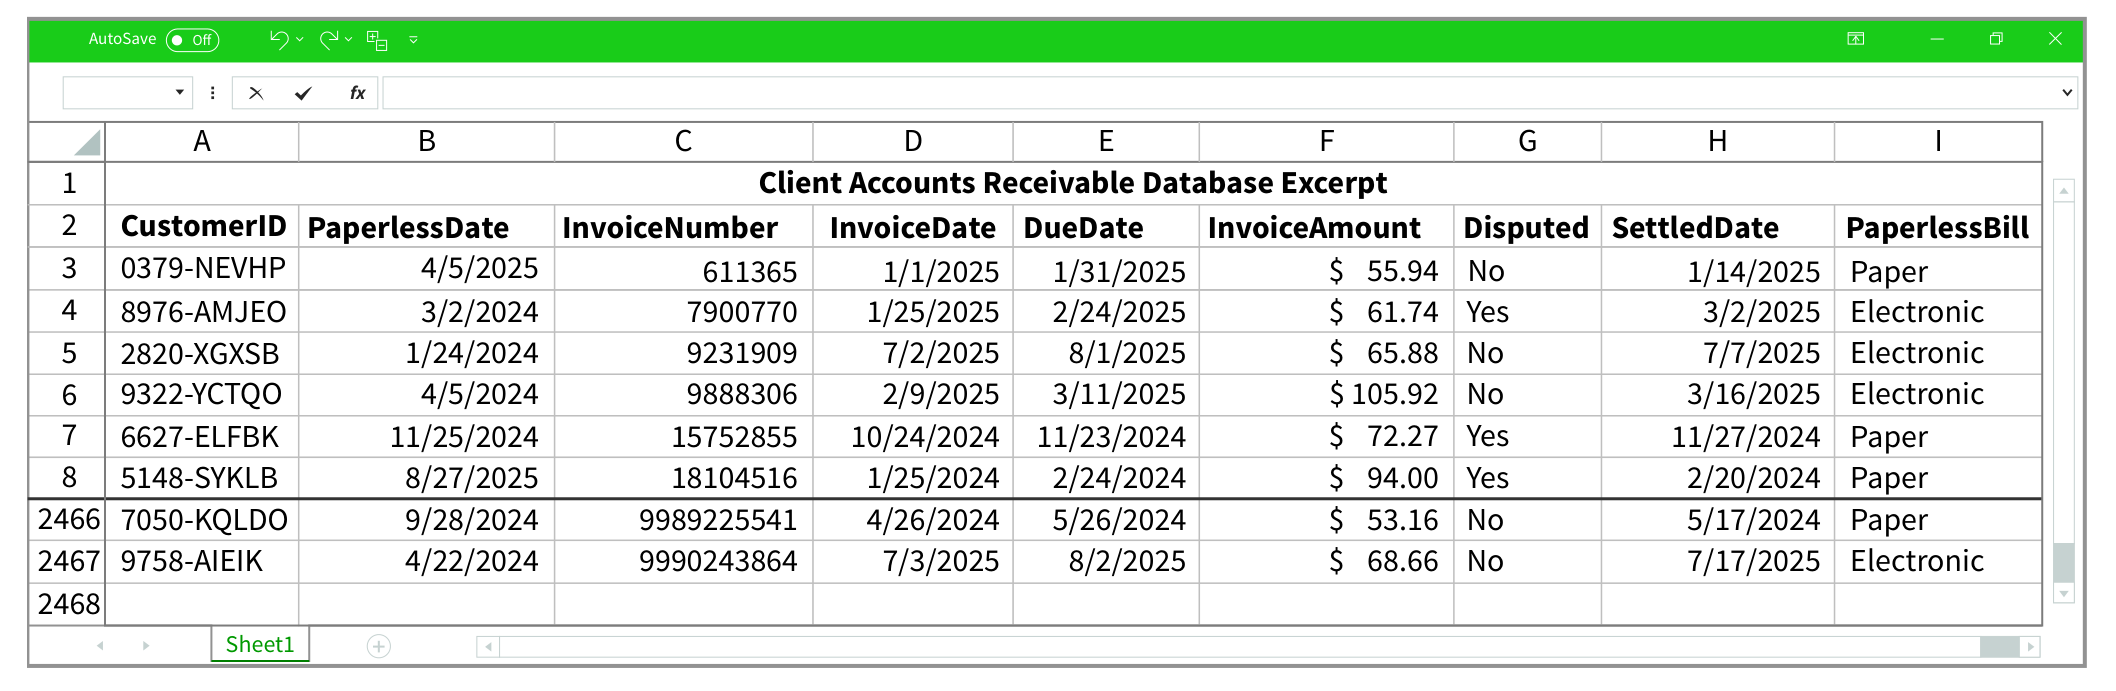
\includegraphics[width=0.95\textwidth,height=0.75\textheight,keepaspectratio]{../textbookForPractice/Figures/Ch_08/ILLUSTRATION 8.1.png}
    \end{figure}
\end{frame}

\begin{frame}{ILLUSTRATION 8.2}

    \begin{figure}[h]
        \centering
        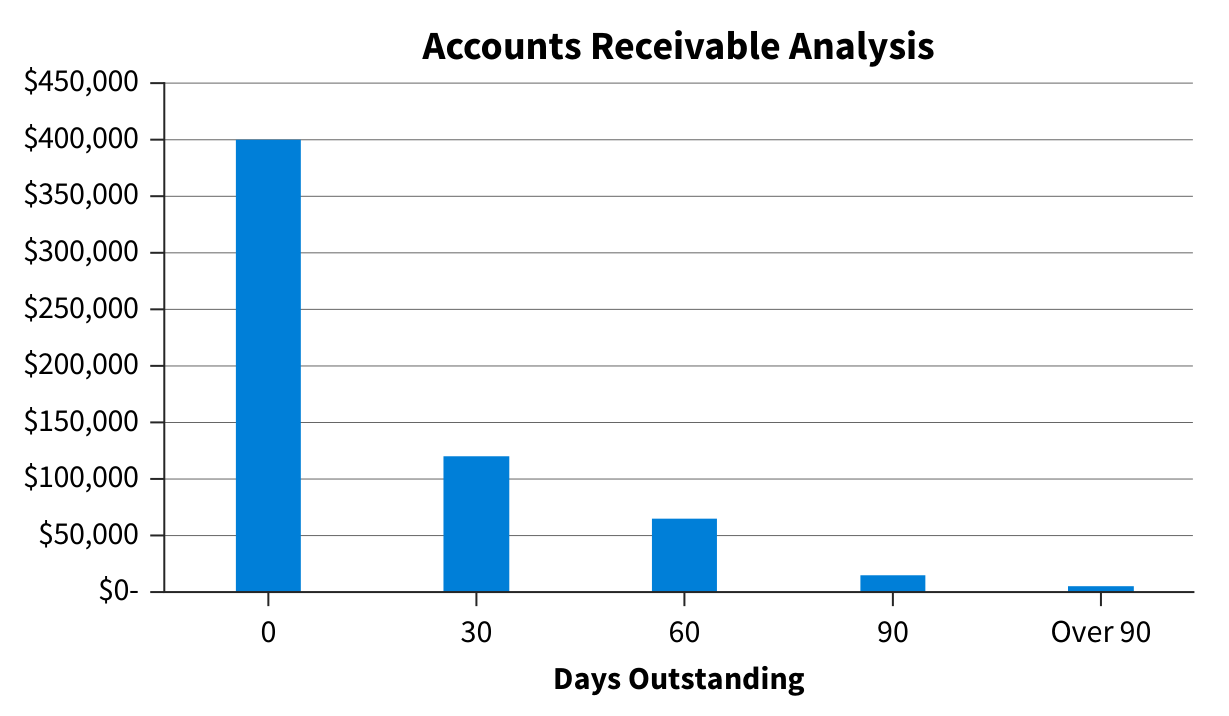
\includegraphics[width=0.95\textwidth,height=0.75\textheight,keepaspectratio]{../textbookForPractice/Figures/Ch_08/ILLUSTRATION 8.2.png}
    \end{figure}
\end{frame}

\begin{frame}{ILLUSTRATION 8.3}

    \begin{figure}[h]
        \centering
        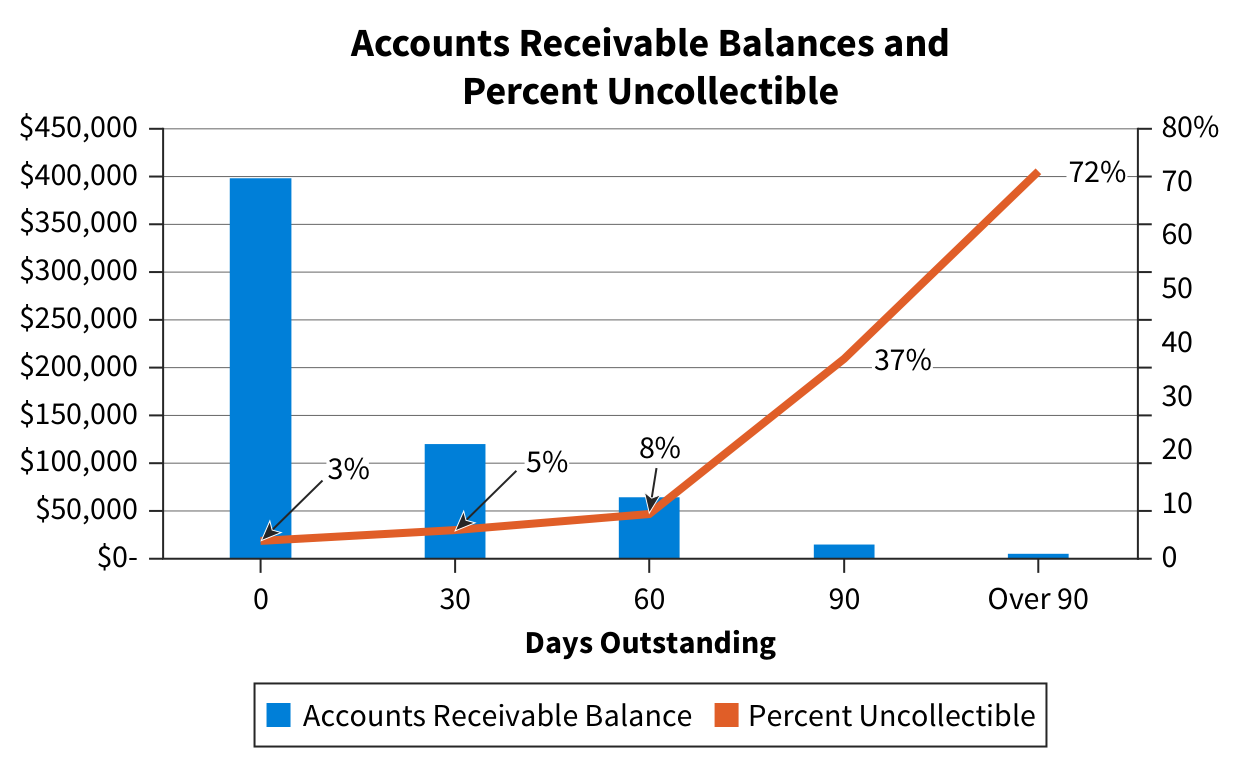
\includegraphics[width=0.95\textwidth,height=0.75\textheight,keepaspectratio]{../textbookForPractice/Figures/Ch_08/ILLUSTRATION 8.3.png}
    \end{figure}
\end{frame}

\begin{frame}{ILLUSTRATION 8.4}

    \begin{figure}[h]
        \centering
        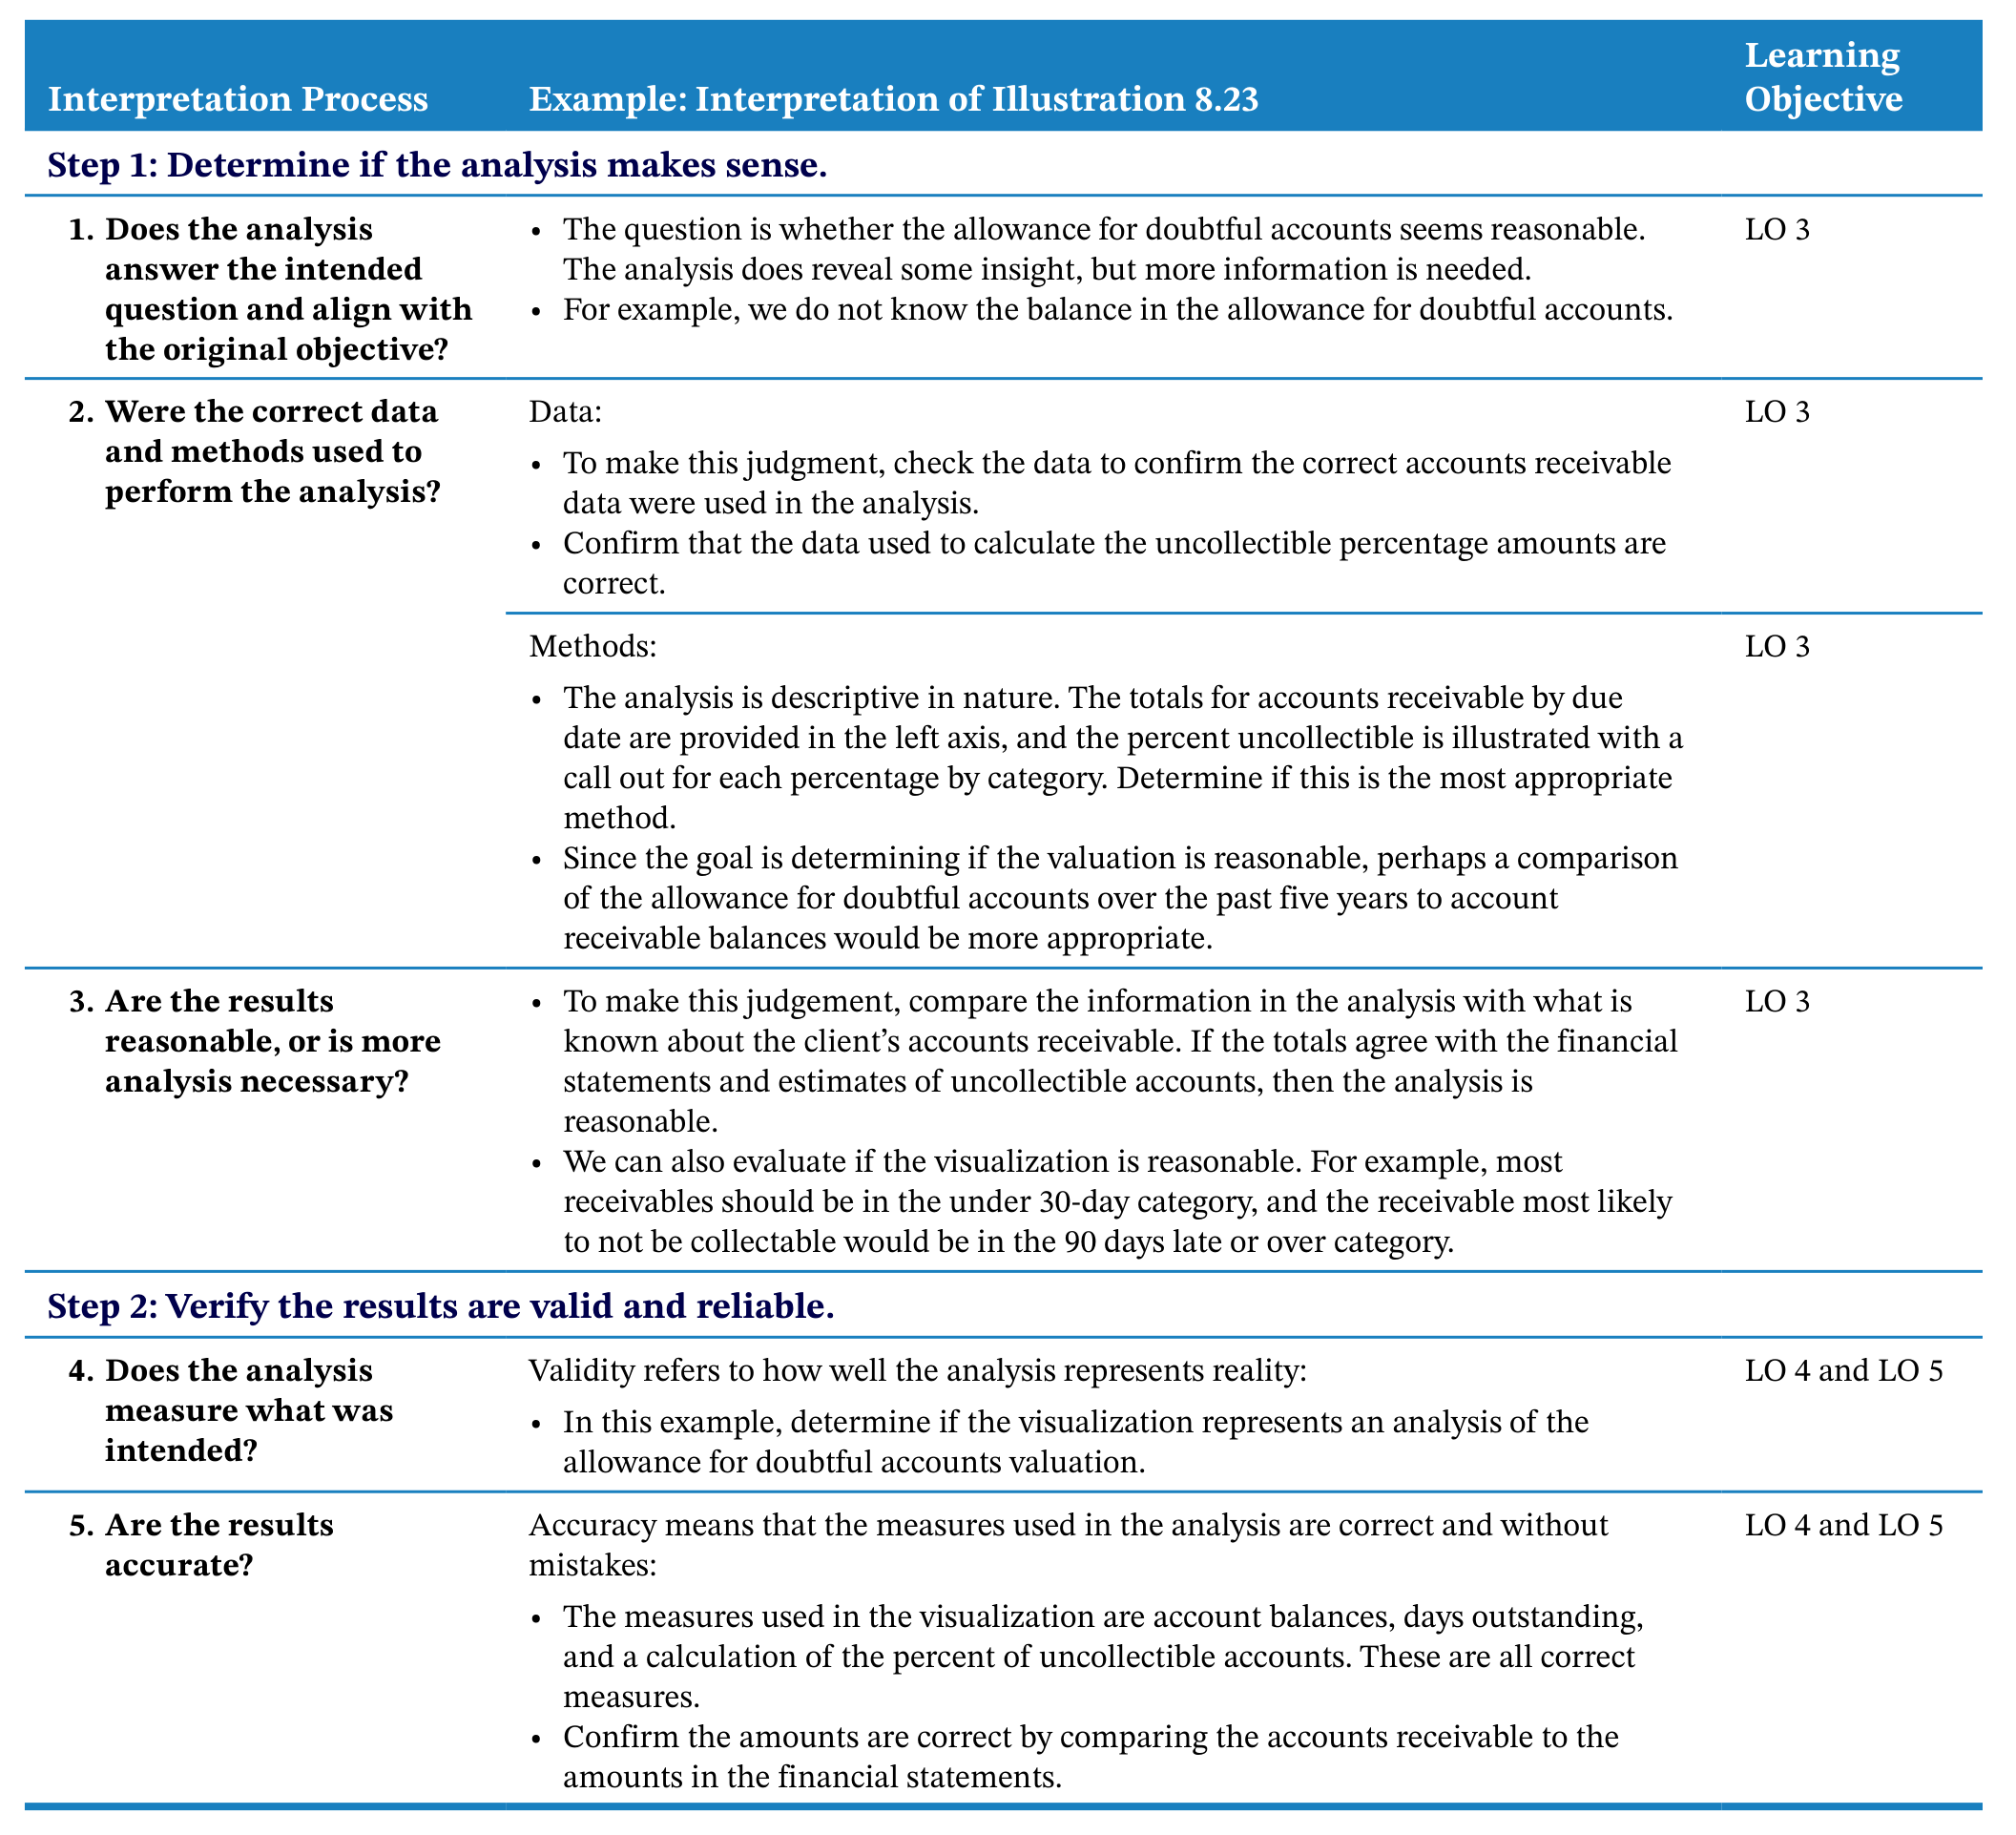
\includegraphics[width=0.95\textwidth,height=0.75\textheight,keepaspectratio]{../textbookForPractice/Figures/Ch_08/ILLUSTRATION 8.4.png}
    \end{figure}
\end{frame}

\begin{frame}{Từ Trực quan hóa đến Diễn giải}
\begin{itemize}
    \item \textbf{Ví dụ:} Một biểu đồ doanh thu đang đi xuống.
    \item \textbf{Khám phá:} Phát hiện ra doanh thu tháng 10 giảm 15\% so với tháng 9.
    \item \textbf{Diễn giải:} Nguyên nhân là do gián đoạn chuỗi cung ứng hoặc thay đổi chính sách tín dụng? Hậu quả là dòng tiền tháng 11 sẽ bị thiếu hụt.
\end{itemize}
\end{frame}

\begin{frame}{ILLUSTRATION 8.5}

    \begin{figure}[h]
        \centering
        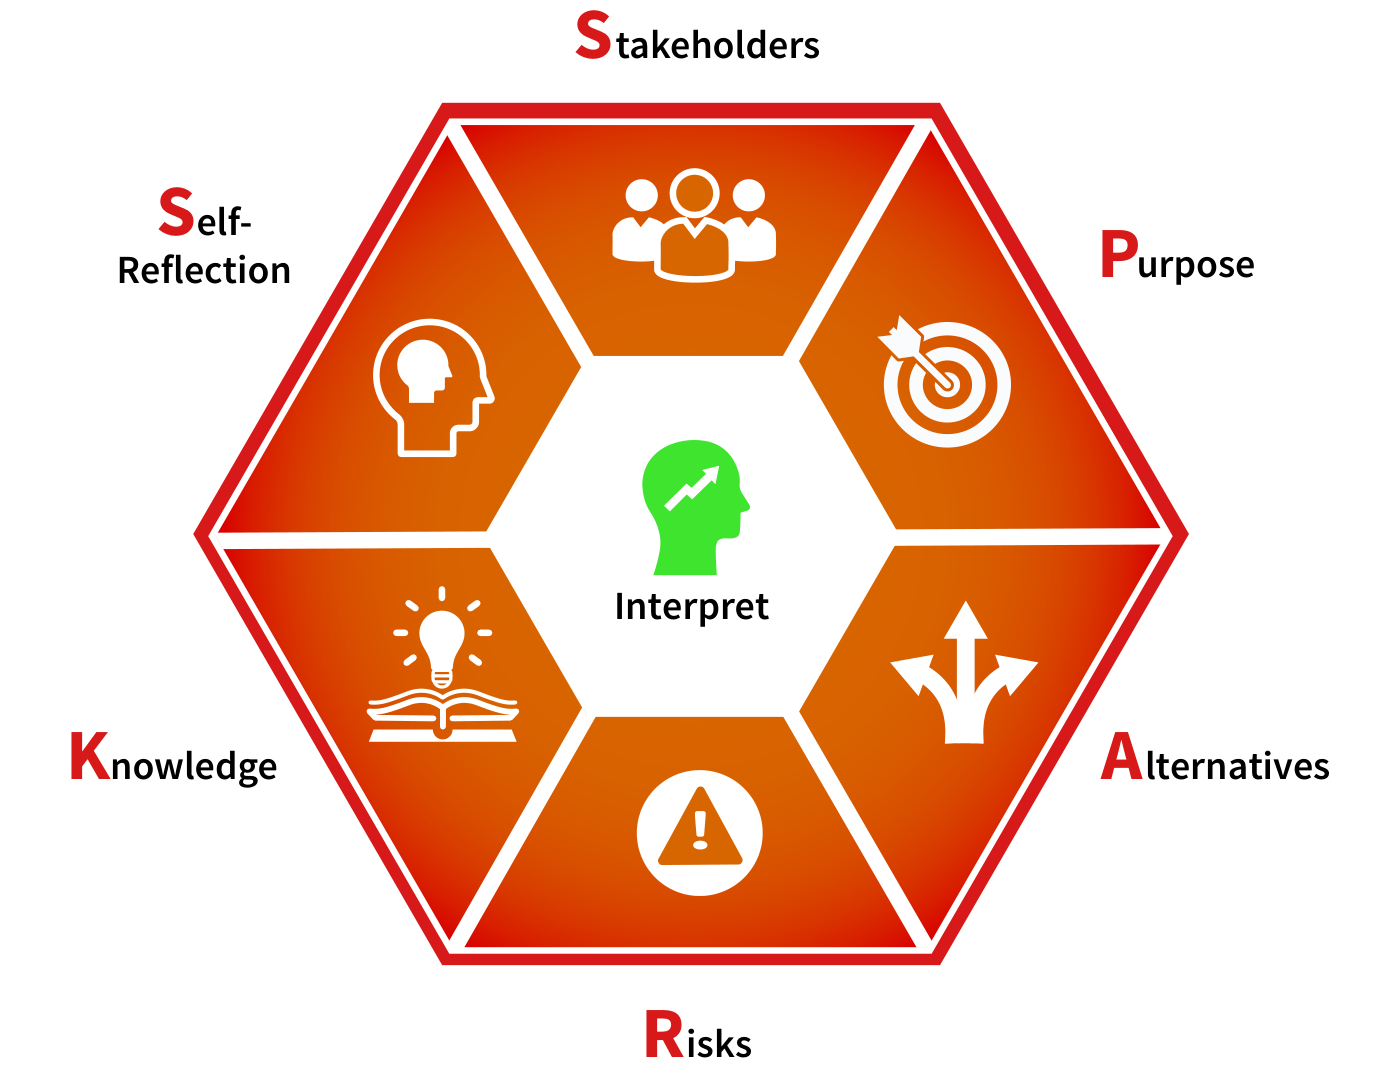
\includegraphics[width=0.95\textwidth,height=0.75\textheight,keepaspectratio]{../textbookForPractice/Figures/Ch_08/ILLUSTRATION 8.5.png}
    \end{figure}
\end{frame}

\begin{frame}{ILLUSTRATION 8.6}

    \begin{figure}[h]
        \centering
        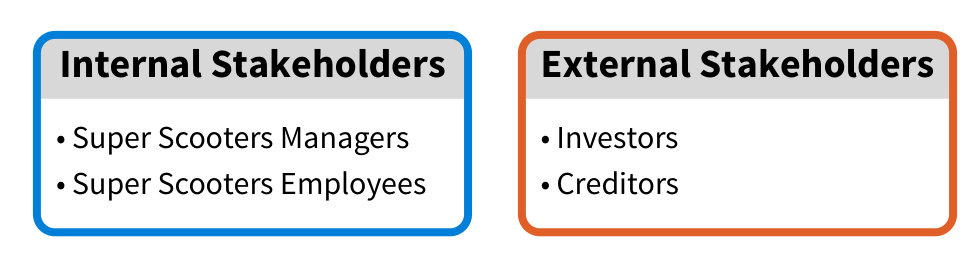
\includegraphics[width=0.95\textwidth,height=0.75\textheight,keepaspectratio]{../textbookForPractice/Figures/Ch_08/ILLUSTRATION 8.6.png}
    \end{figure}
\end{frame}

\begin{frame}{ILLUSTRATION 8.7}

    \begin{figure}[h]
        \centering
        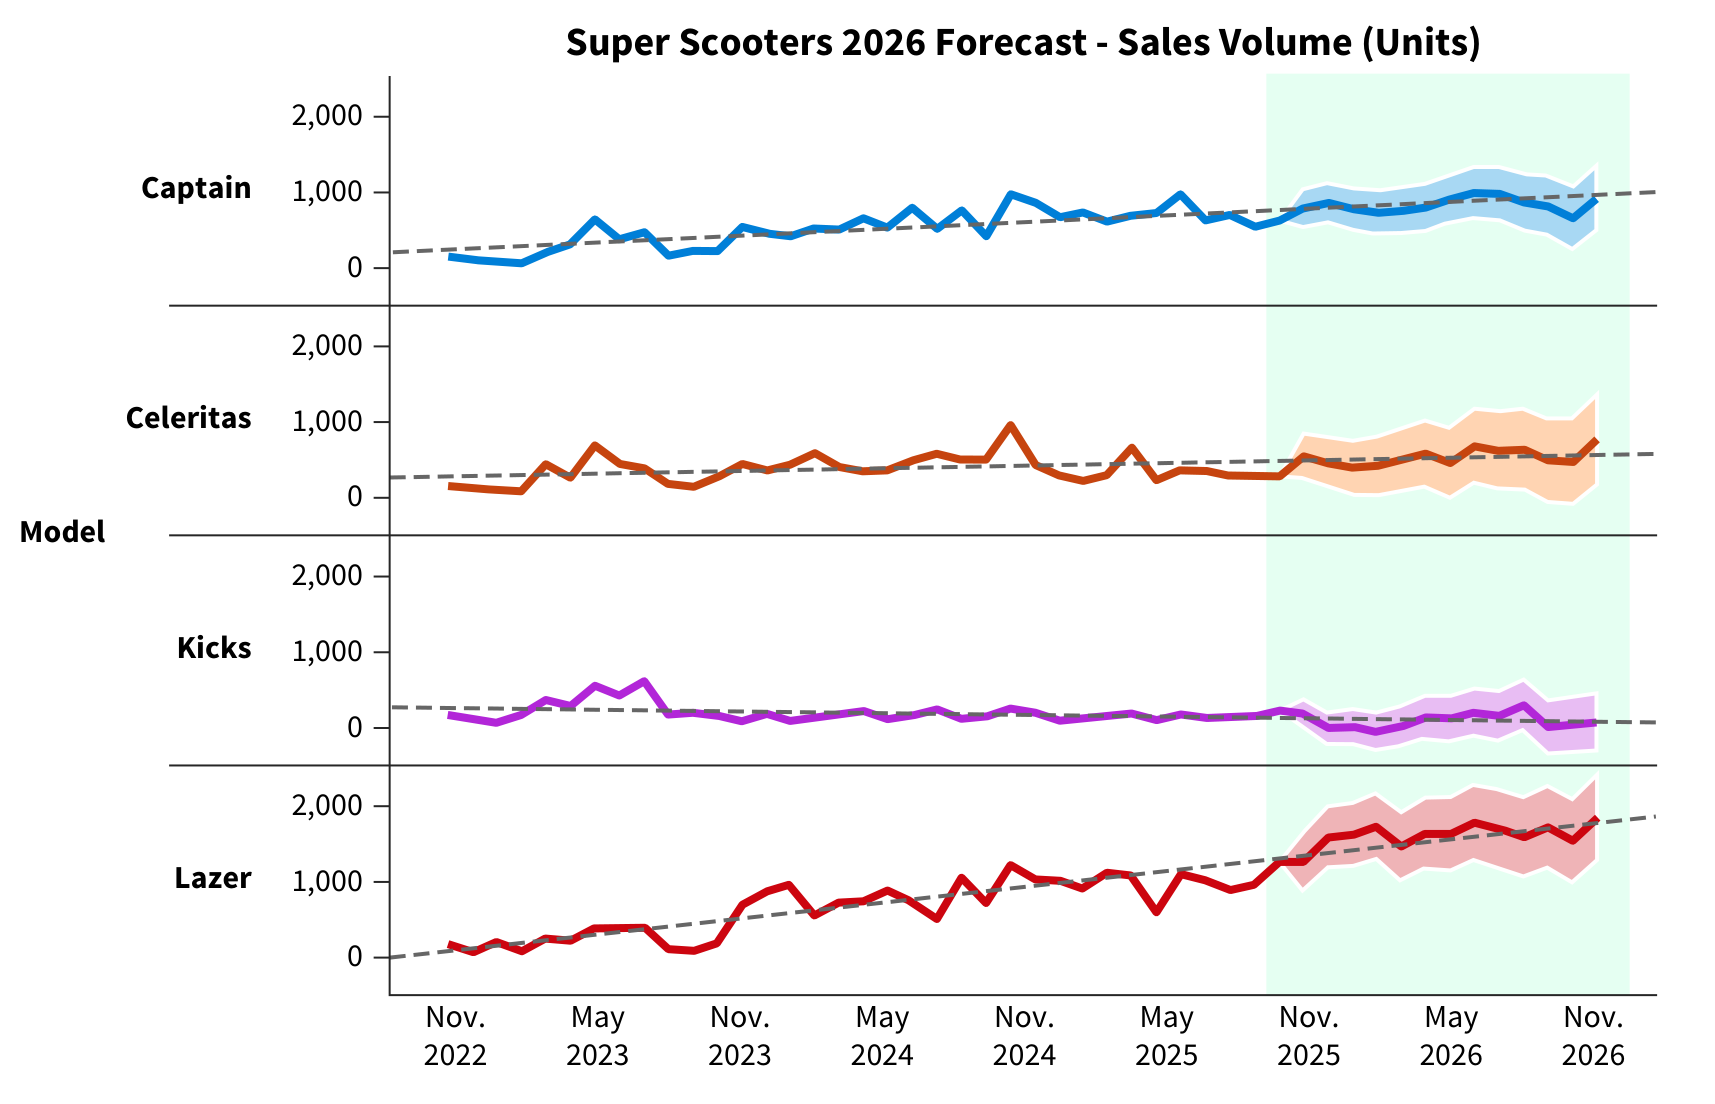
\includegraphics[width=0.95\textwidth,height=0.75\textheight,keepaspectratio]{../textbookForPractice/Figures/Ch_08/ILLUSTRATION 8.7.png}
    \end{figure}
\end{frame}

\begin{frame}{ILLUSTRATION 8.8}

    \begin{figure}[h]
        \centering
        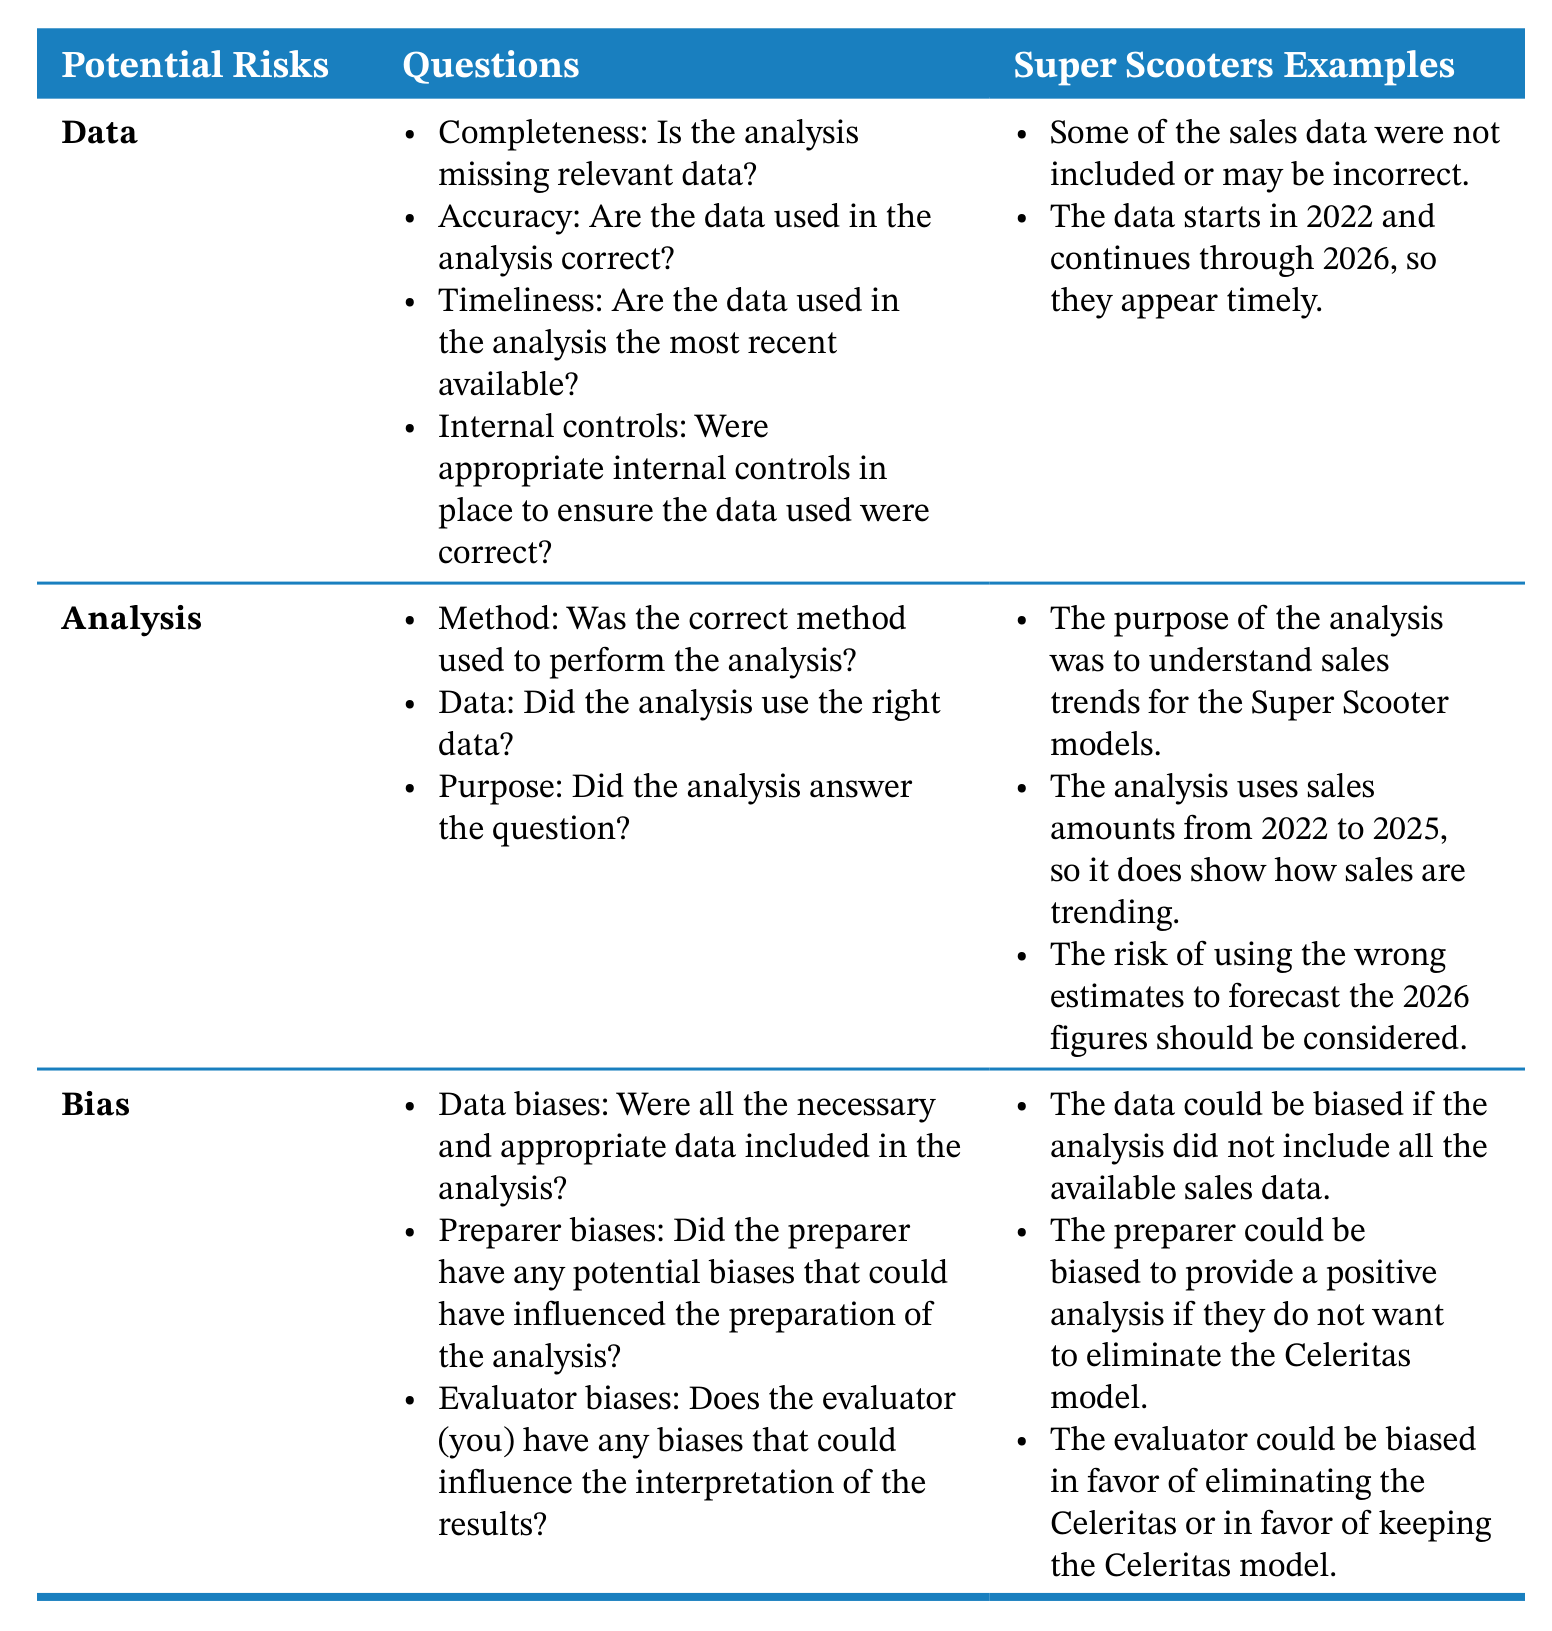
\includegraphics[width=0.95\textwidth,height=0.75\textheight,keepaspectratio]{../textbookForPractice/Figures/Ch_08/ILLUSTRATION 8.8.png}
    \end{figure}
\end{frame}

\begin{frame}{8.2 Ứng dụng Tư duy Phản biện (SPARK-S)}
\begin{itemize}
    \item Tư duy phản biện giúp chúng ta không bị dẫn dắt bởi những dữ liệu sai lệch hoặc thiên kiến. Khung \textbf{SPARK-S}:
    \begin{itemize}
        \item \textbf{S - Stakeholders:} Ai bị ảnh hưởng bởi kết quả này?
        \item \textbf{P - Purpose:} Mục đích ban đầu của việc phân tích là gì?
        \item \textbf{A - Alternatives:} Có cách giải thích nào khác cho hiện tượng này không?
    \end{itemize}
\end{itemize}
\end{frame}

\begin{frame}{ILLUSTRATION 8.9}

    \begin{figure}[h]
        \centering
        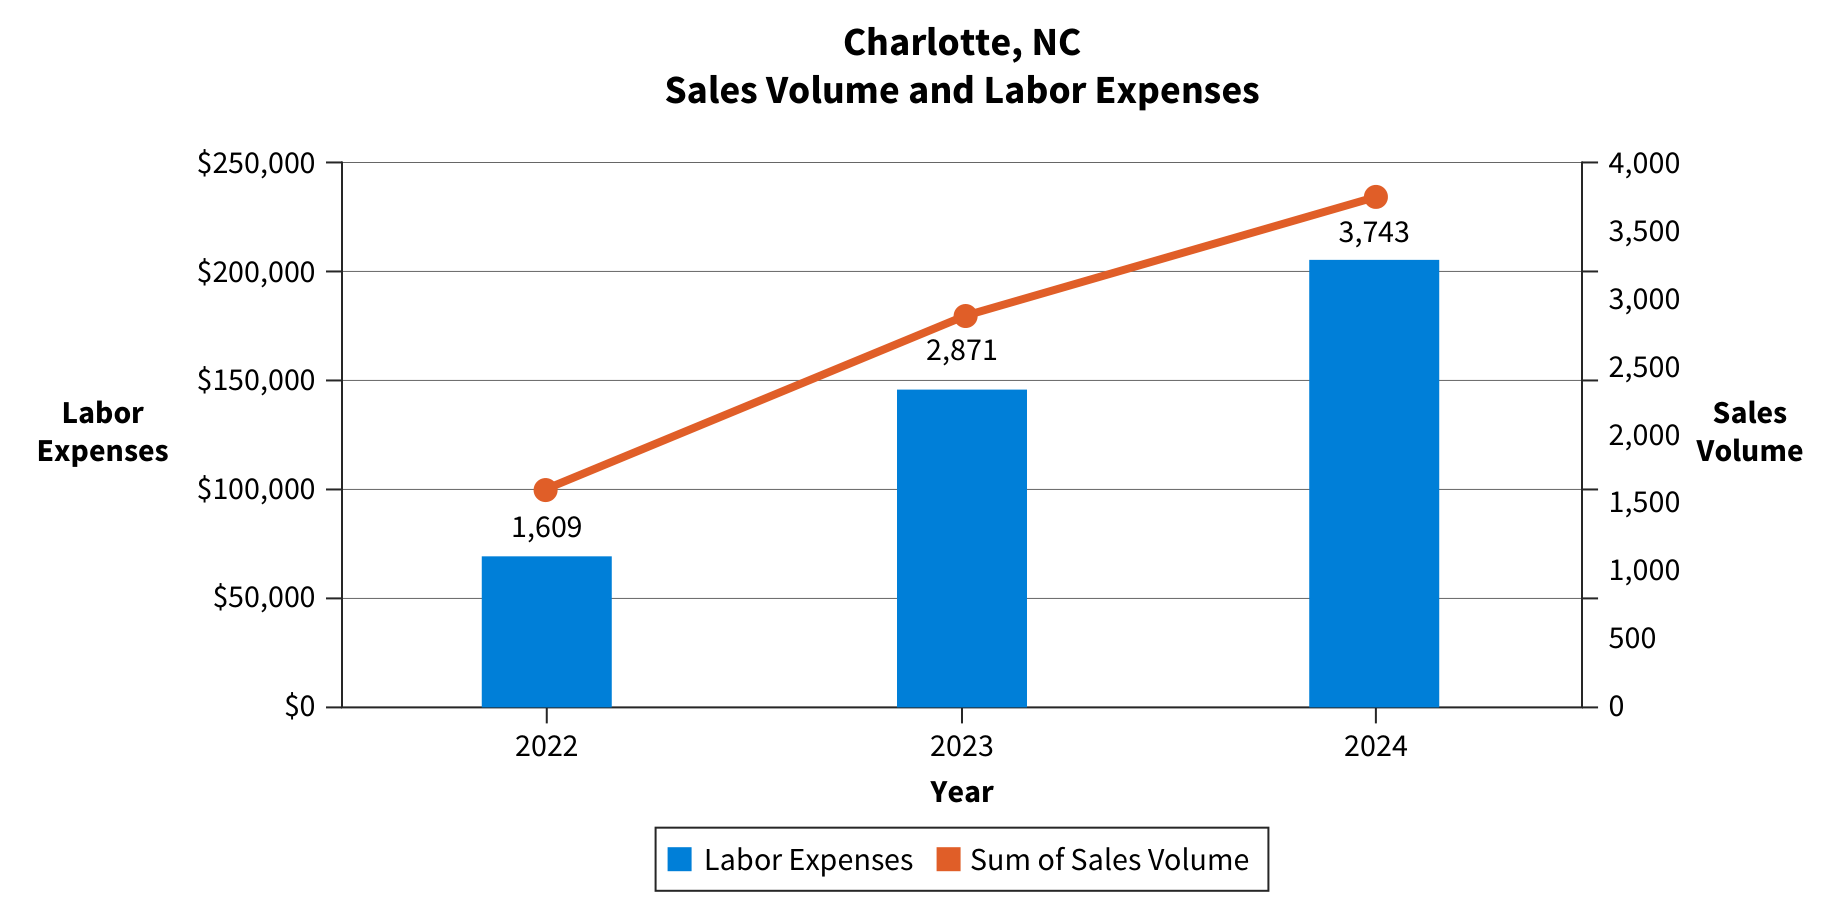
\includegraphics[width=0.95\textwidth,height=0.75\textheight,keepaspectratio]{../textbookForPractice/Figures/Ch_08/ILLUSTRATION 8.9.png}
    \end{figure}
\end{frame}

\begin{frame}{ILLUSTRATION 8.10}

    \begin{figure}[h]
        \centering
        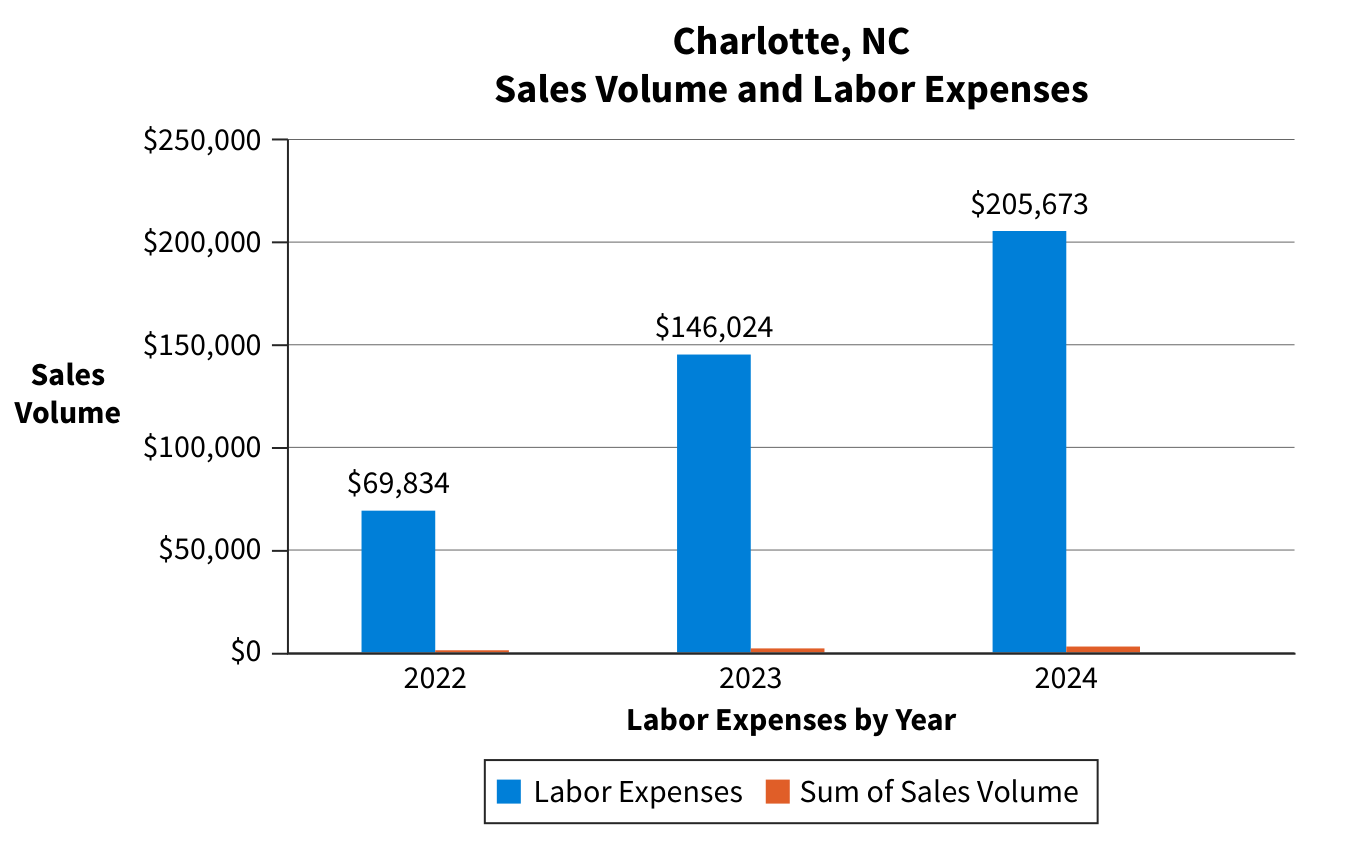
\includegraphics[width=0.95\textwidth,height=0.75\textheight,keepaspectratio]{../textbookForPractice/Figures/Ch_08/ILLUSTRATION 8.10.png}
    \end{figure}
\end{frame}

\begin{frame}{ILLUSTRATION 8.11}

    \begin{figure}[h]
        \centering
        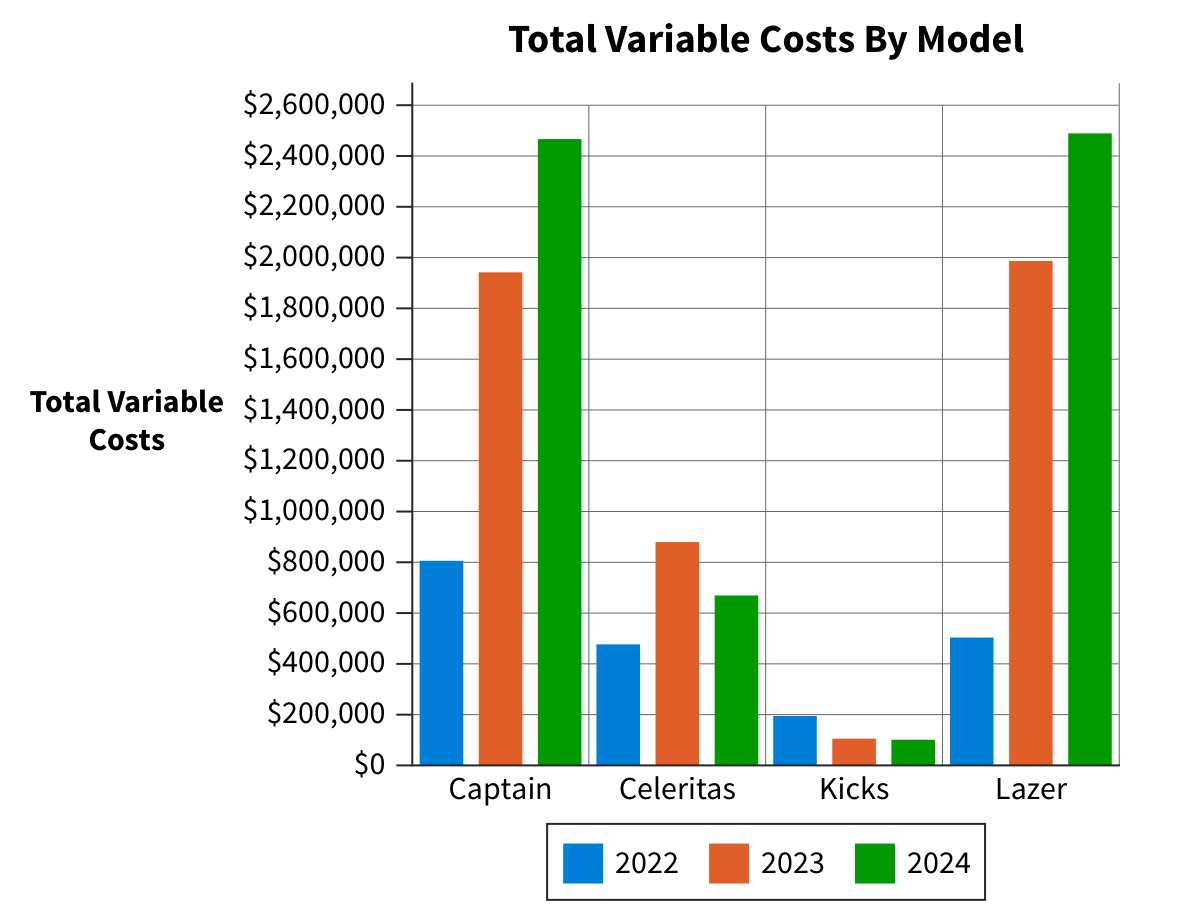
\includegraphics[width=0.95\textwidth,height=0.75\textheight,keepaspectratio]{../textbookForPractice/Figures/Ch_08/ILLUSTRATION 8.11.png}
    \end{figure}
\end{frame}

\begin{frame}{ILLUSTRATION 8.12}

    \begin{figure}[h]
        \centering
        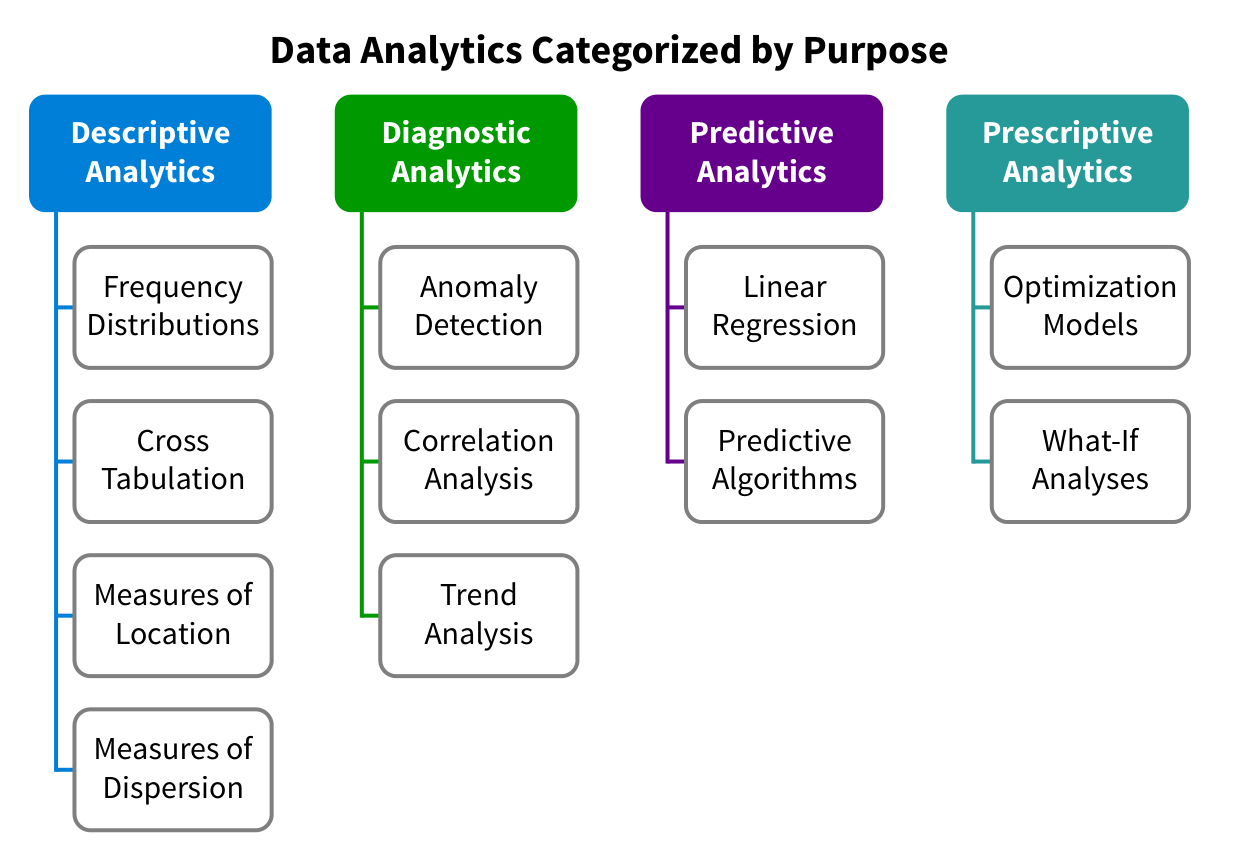
\includegraphics[width=0.95\textwidth,height=0.75\textheight,keepaspectratio]{../textbookForPractice/Figures/Ch_08/ILLUSTRATION 8.12.png}
    \end{figure}
\end{frame}

\begin{frame}{Tư duy Phản biện (Tiếp theo)}
\begin{itemize}
    \item \textbf{Khung SPARK-S (Tiếp):}
    \begin{itemize}
        \item \textbf{R - Risks \& Biases:} Phân tích này có gặp phải thiên kiến xác nhận (Confirmation Bias) hay rủi ro dữ liệu sai không?
        \item \textbf{K - Knowledge:} Chúng ta cần thêm thông tin gì để kết luận chắc chắn hơn?
        \item \textbf{S - Self-reflection:} Đánh giá lại bản thân trong quá trình phân tích.
    \end{itemize}
\end{itemize}
\end{frame}

\begin{frame}{ILLUSTRATION 8.13}

    \begin{figure}[h]
        \centering
        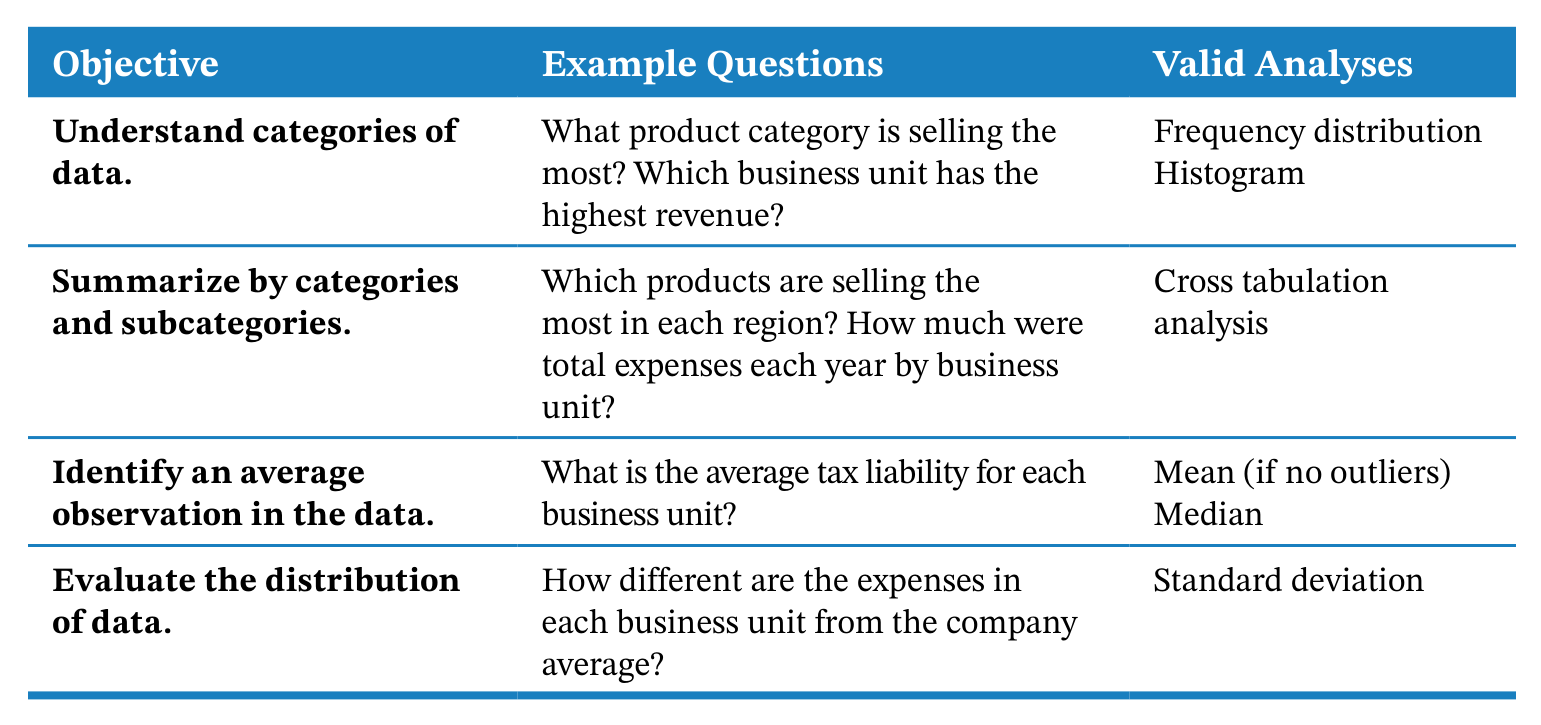
\includegraphics[width=0.95\textwidth,height=0.75\textheight,keepaspectratio]{../textbookForPractice/Figures/Ch_08/ILLUSTRATION 8.13.png}
    \end{figure}
\end{frame}

\begin{frame}{ILLUSTRATION 8.14}

    \begin{figure}[h]
        \centering
        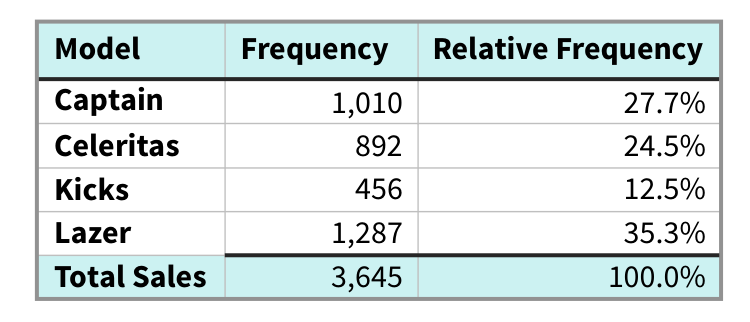
\includegraphics[width=0.95\textwidth,height=0.75\textheight,keepaspectratio]{../textbookForPractice/Figures/Ch_08/ILLUSTRATION 8.14.png}
    \end{figure}
\end{frame}

\begin{frame}{ILLUSTRATION 8.15}

    \begin{figure}[h]
        \centering
        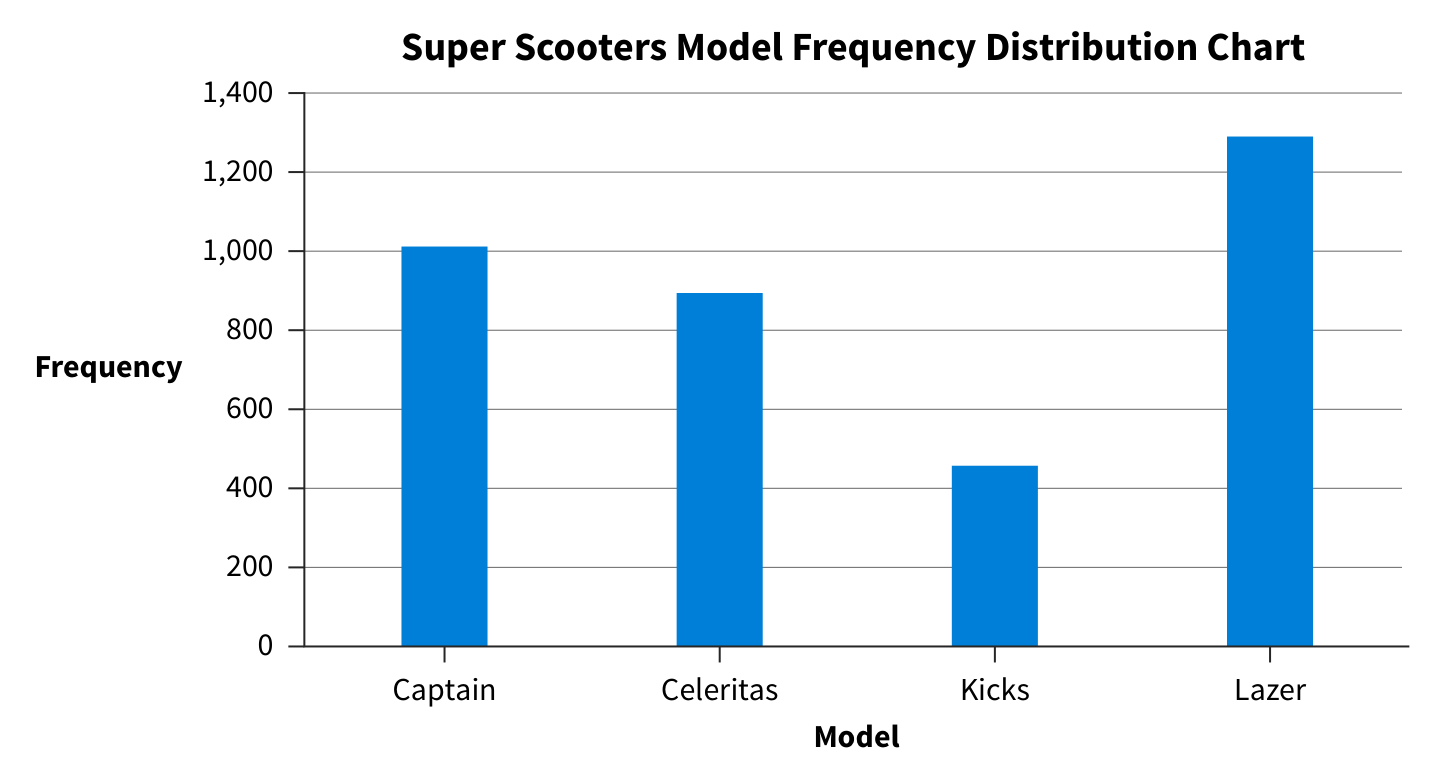
\includegraphics[width=0.95\textwidth,height=0.75\textheight,keepaspectratio]{../textbookForPractice/Figures/Ch_08/ILLUSTRATION 8.15.png}
    \end{figure}
\end{frame}

\begin{frame}{ILLUSTRATION 8.16}

    \begin{figure}[h]
        \centering
        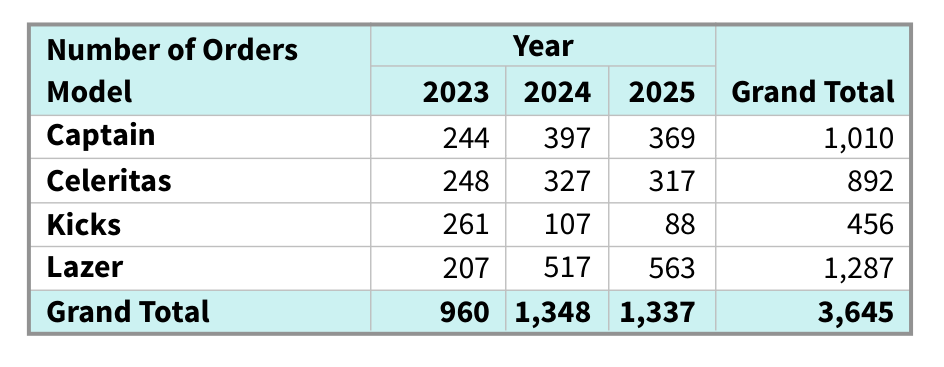
\includegraphics[width=0.95\textwidth,height=0.75\textheight,keepaspectratio]{../textbookForPractice/Figures/Ch_08/ILLUSTRATION 8.16.png}
    \end{figure}
\end{frame}

\begin{frame}{8.3 Đánh giá Sự phù hợp của Kết quả}
\begin{itemize}
    \item \textbf{Câu hỏi chính:} Kết quả thu được có thực sự \textit{trả lời được câu hỏi kinh doanh} ban đầu không?
    \item \textbf{Đánh giá Dữ liệu (Data):} Dữ liệu có đủ sạch, đủ lớn và đại diện cho vấn đề không?
    \item \textbf{Đánh giá Phương pháp (Methods):} Mô hình thống kê hoặc biểu đồ được chọn có phù hợp với loại dữ liệu không?
\end{itemize}
\end{frame}

\begin{frame}{ILLUSTRATION 8.17}

    \begin{figure}[h]
        \centering
        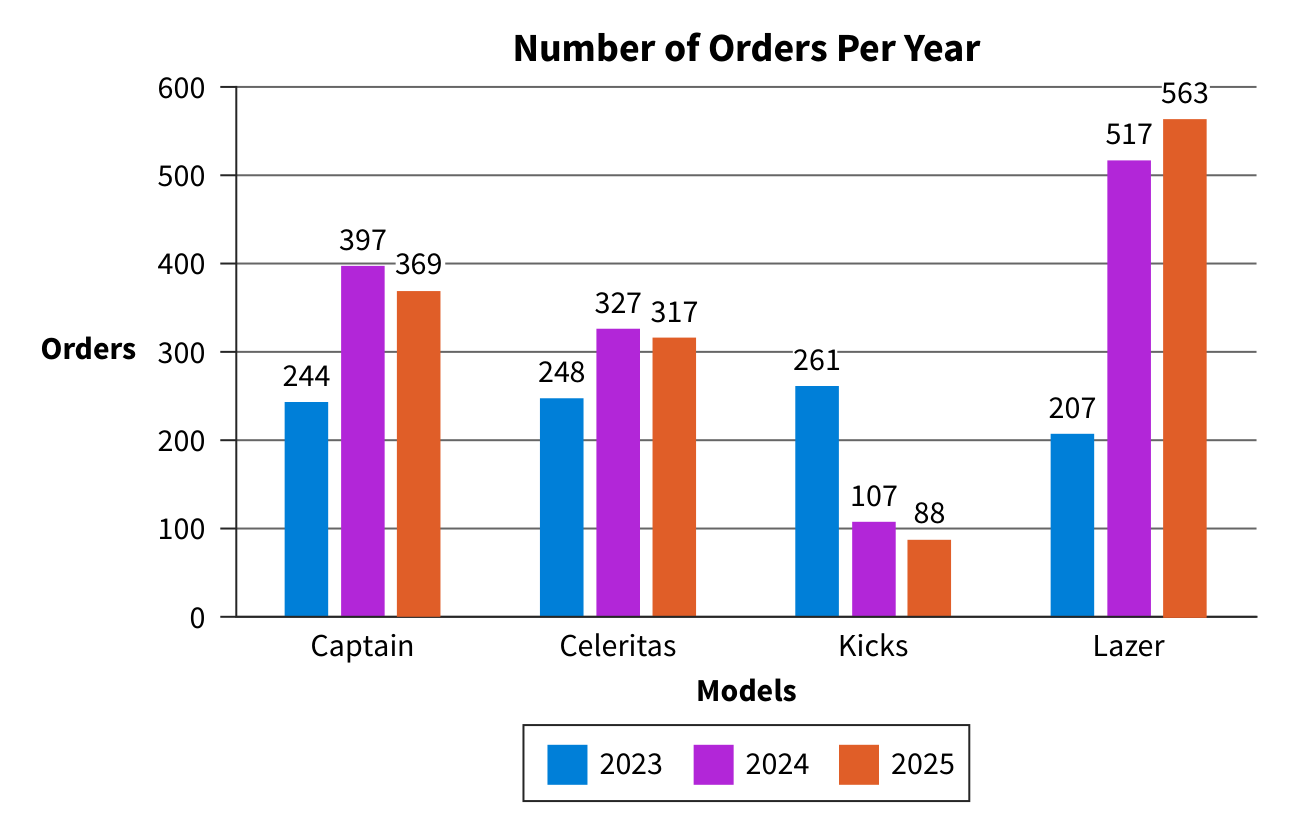
\includegraphics[width=0.95\textwidth,height=0.75\textheight,keepaspectratio]{../textbookForPractice/Figures/Ch_08/ILLUSTRATION 8.17.png}
    \end{figure}
\end{frame}

\begin{frame}{ILLUSTRATION 8.18}

    \begin{figure}[h]
        \centering
        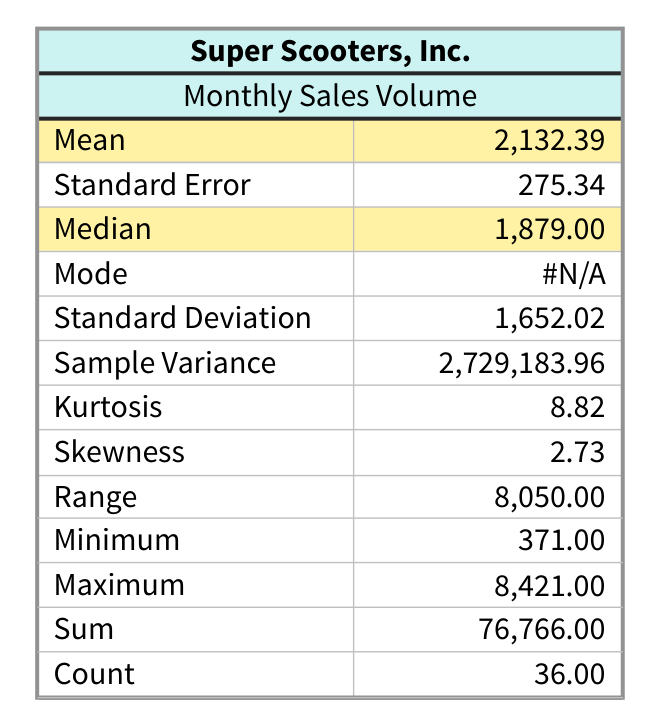
\includegraphics[width=0.95\textwidth,height=0.75\textheight,keepaspectratio]{../textbookForPractice/Figures/Ch_08/ILLUSTRATION 8.18.png}
    \end{figure}
\end{frame}

\begin{frame}{ILLUSTRATION 8.19}

    \begin{figure}[h]
        \centering
        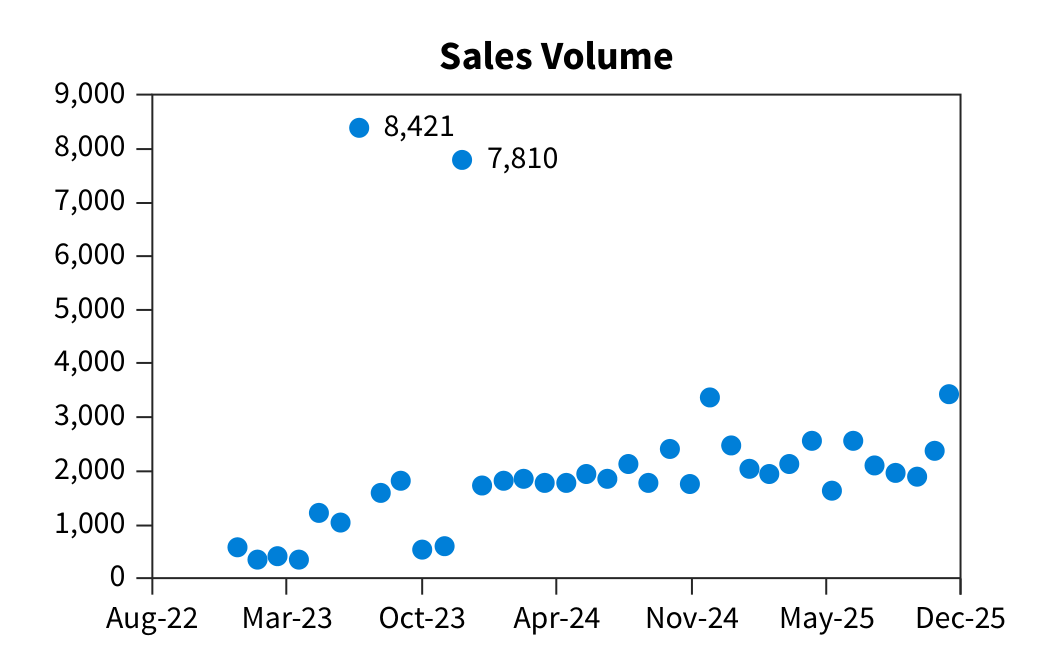
\includegraphics[width=0.95\textwidth,height=0.75\textheight,keepaspectratio]{../textbookForPractice/Figures/Ch_08/ILLUSTRATION 8.19.png}
    \end{figure}
\end{frame}

\begin{frame}{ILLUSTRATION 8.20}

    \begin{figure}[h]
        \centering
        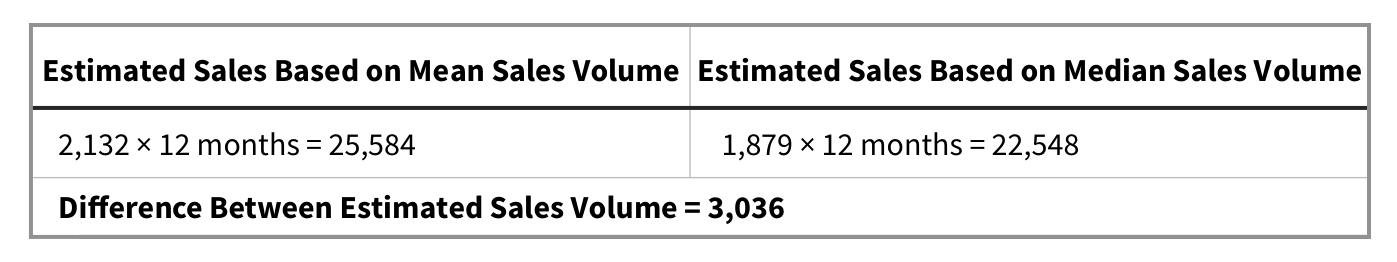
\includegraphics[width=0.95\textwidth,height=0.75\textheight,keepaspectratio]{../textbookForPractice/Figures/Ch_08/ILLUSTRATION 8.20.png}
    \end{figure}
\end{frame}

\begin{frame}{Kiểm tra và Bổ sung thông tin}
\begin{itemize}
    \item \textbf{Kiểm tra Kết quả (Examine Results):} Các con số có ý nghĩa thực tế không? (Ví dụ: Tỷ suất lợi nhuận 500\% có thể là do lỗi dữ liệu hơn là thực tế).
    \item \textbf{Xác định thông tin cần thêm:} Có cần bổ sung dữ liệu phi tài chính (Non-financial data) để giải thích cho dữ liệu tài chính không?
\end{itemize}
\end{frame}

\begin{frame}{ILLUSTRATION 8.21}

    \begin{figure}[h]
        \centering
        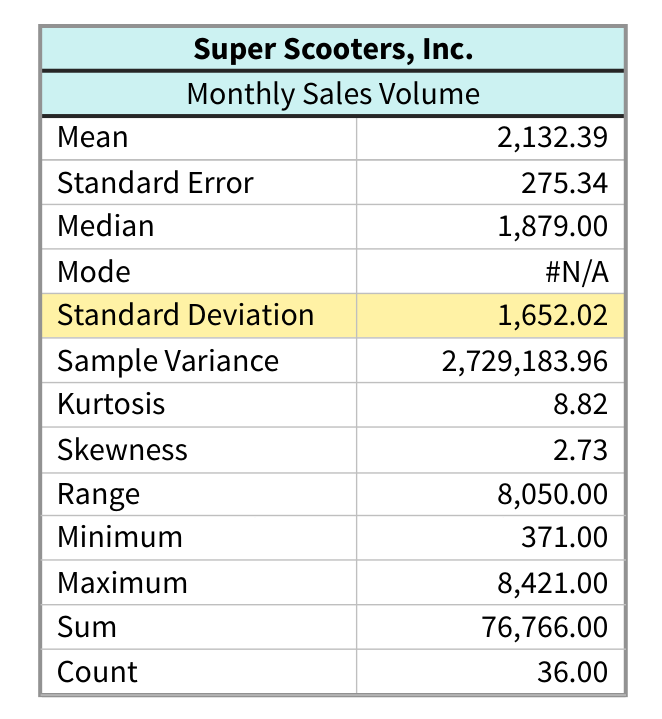
\includegraphics[width=0.95\textwidth,height=0.75\textheight,keepaspectratio]{../textbookForPractice/Figures/Ch_08/ILLUSTRATION 8.21.png}
    \end{figure}
\end{frame}

\begin{frame}{ILLUSTRATION 8.22}

    \begin{figure}[h]
        \centering
        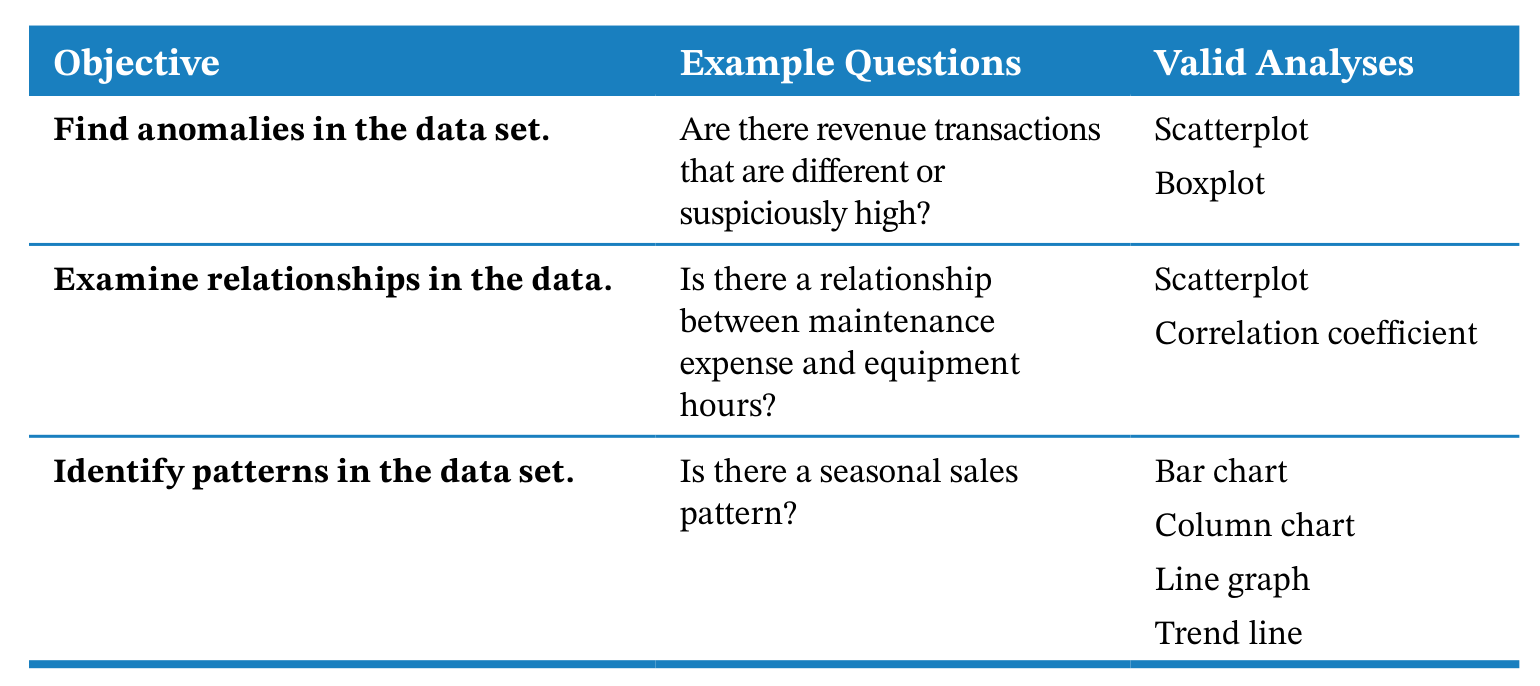
\includegraphics[width=0.95\textwidth,height=0.75\textheight,keepaspectratio]{../textbookForPractice/Figures/Ch_08/ILLUSTRATION 8.22.png}
    \end{figure}
\end{frame}

\begin{frame}{ILLUSTRATION 8.23}

    \begin{figure}[h]
        \centering
        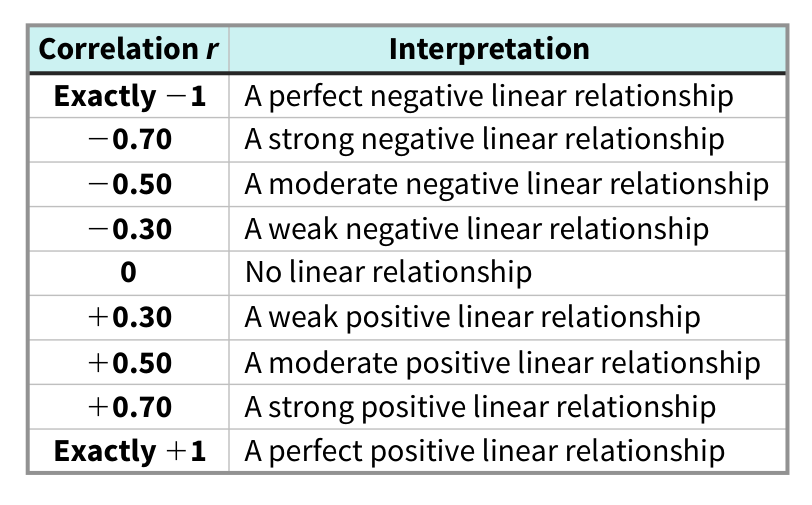
\includegraphics[width=0.95\textwidth,height=0.75\textheight,keepaspectratio]{../textbookForPractice/Figures/Ch_08/ILLUSTRATION 8.23.png}
    \end{figure}
\end{frame}

\begin{frame}{ILLUSTRATION 8.24}

    \begin{figure}[h]
        \centering
        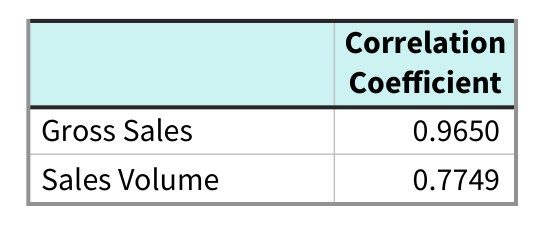
\includegraphics[width=0.95\textwidth,height=0.75\textheight,keepaspectratio]{../textbookForPractice/Figures/Ch_08/ILLUSTRATION 8.24.png}
    \end{figure}
\end{frame}

\begin{frame}{8.4 Đánh giá Phân tích Mô tả và Chẩn đoán}
\begin{itemize}
    \item \textbf{Tính Hợp lệ (Validity):} Đo lường đúng thứ cần đo.
    \item \textbf{Độ Tin cậy (Reliability):} Tính nhất quán của kết quả khi lặp lại phân tích.
    \item \textbf{Phân tích Mô tả (Descriptive):} Đánh giá tính chính xác của các chỉ số tóm tắt (Tổng, Trung bình, Max, Min).
\end{itemize}
\end{frame}

\begin{frame}{ILLUSTRATION 8.25}

    \begin{figure}[h]
        \centering
        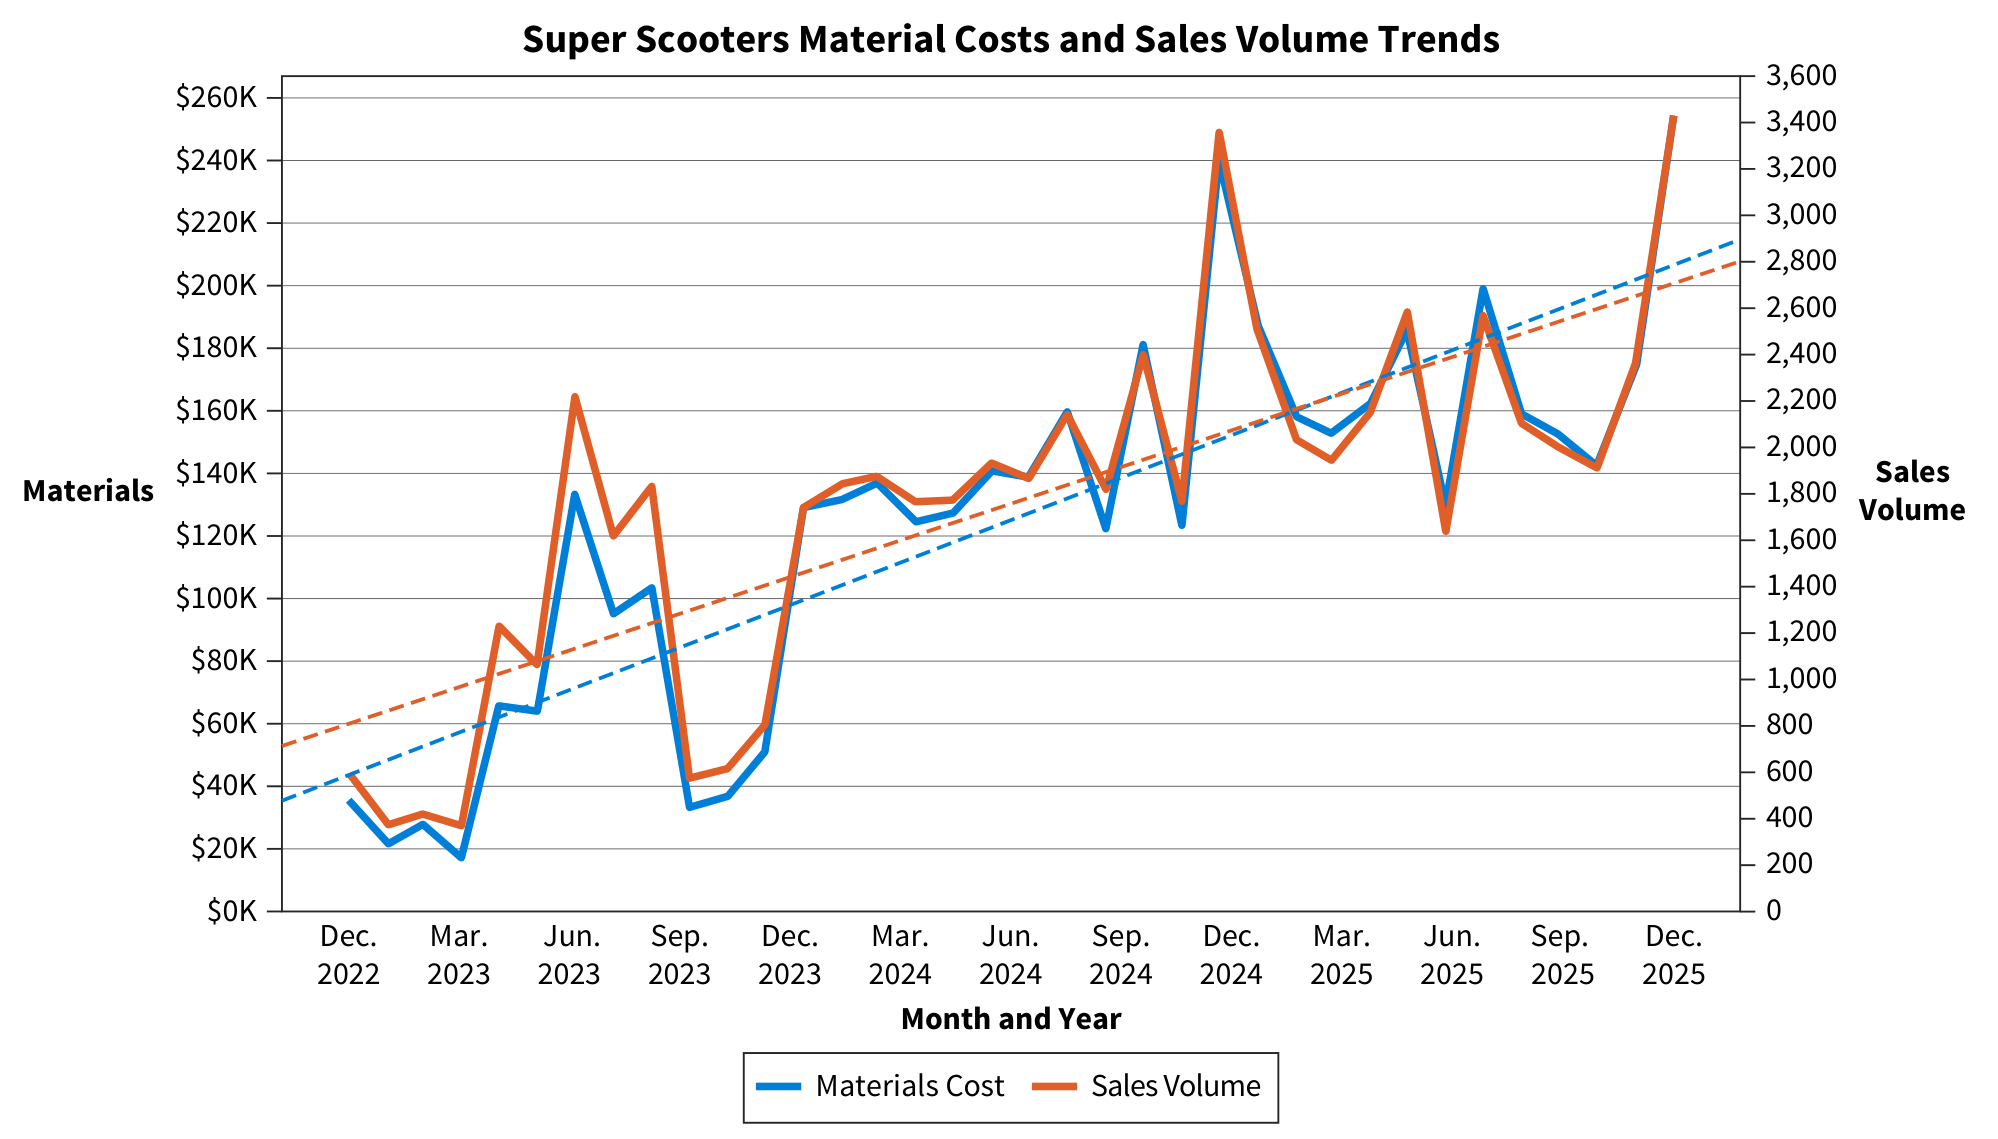
\includegraphics[width=0.95\textwidth,height=0.75\textheight,keepaspectratio]{../textbookForPractice/Figures/Ch_08/ILLUSTRATION 8.25.png}
    \end{figure}
\end{frame}

\begin{frame}{ILLUSTRATION 8.26}

    \begin{figure}[h]
        \centering
        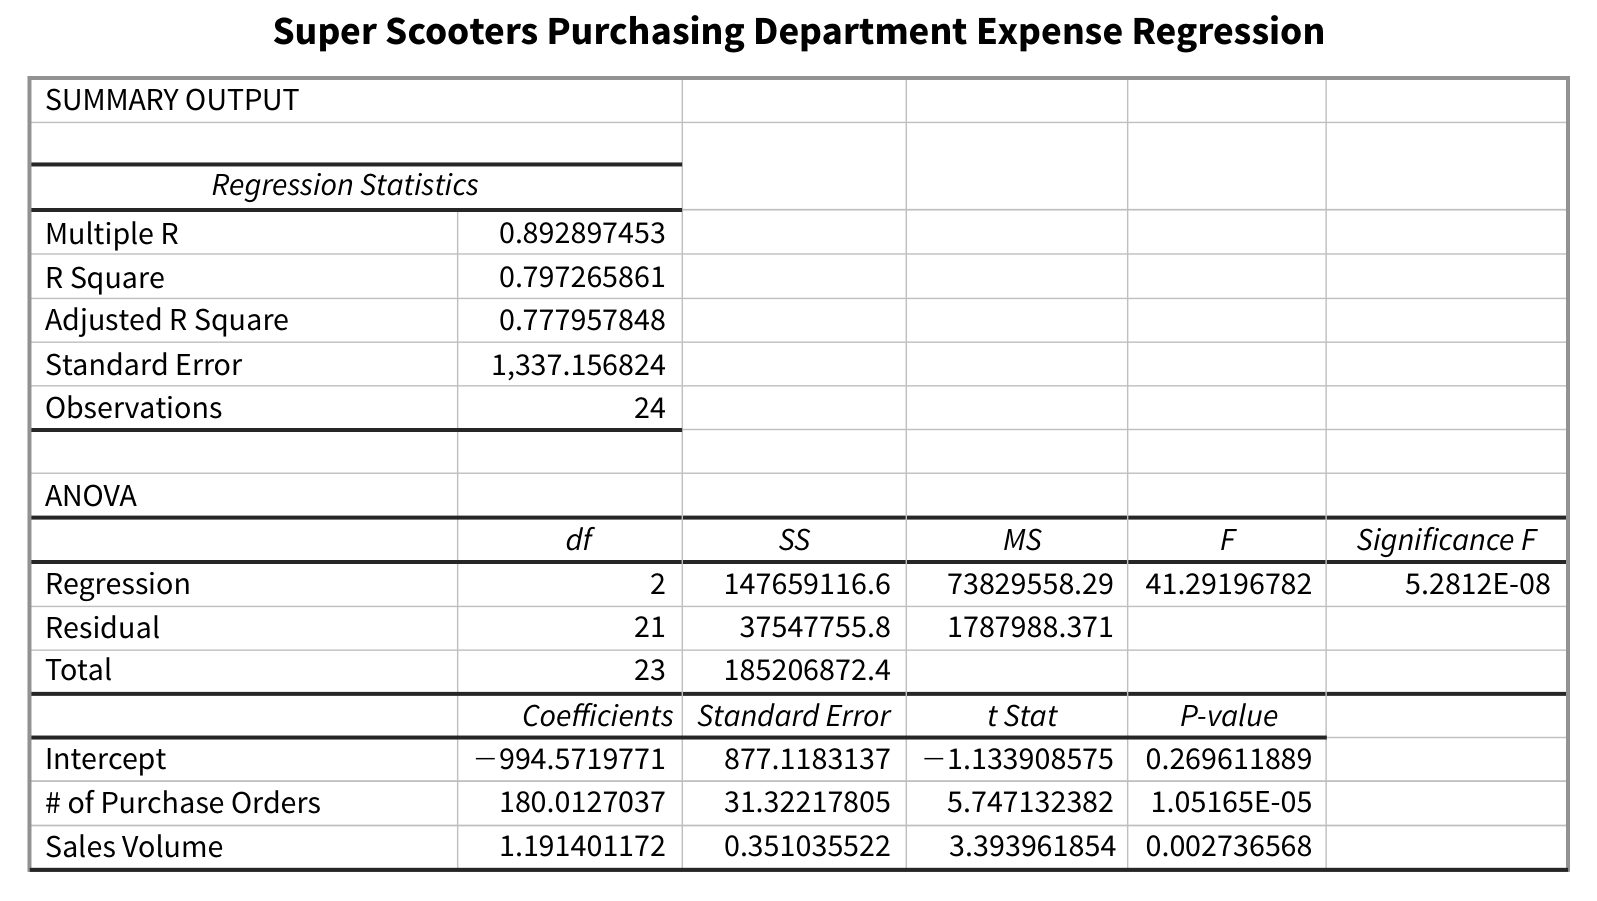
\includegraphics[width=0.95\textwidth,height=0.75\textheight,keepaspectratio]{../textbookForPractice/Figures/Ch_08/ILLUSTRATION 8.26.png}
    \end{figure}
\end{frame}

\begin{frame}{ILLUSTRATION 8.27}

    \begin{figure}[h]
        \centering
        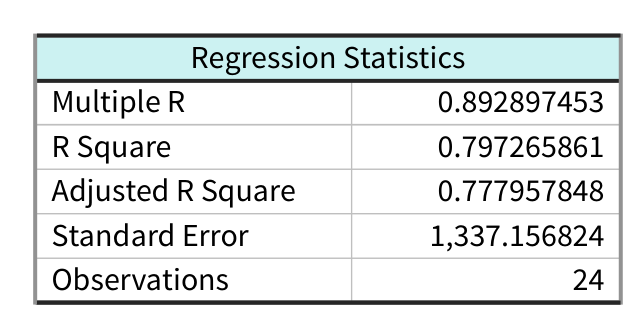
\includegraphics[width=0.95\textwidth,height=0.75\textheight,keepaspectratio]{../textbookForPractice/Figures/Ch_08/ILLUSTRATION 8.27.png}
    \end{figure}
\end{frame}

\begin{frame}{ILLUSTRATION 8.28}

    \begin{figure}[h]
        \centering
        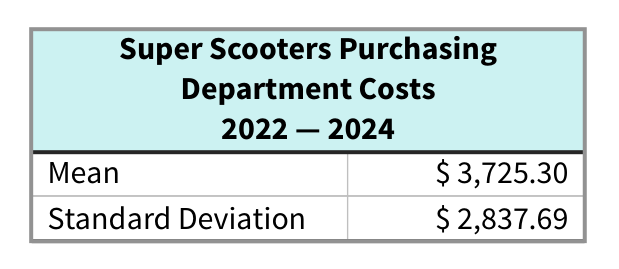
\includegraphics[width=0.95\textwidth,height=0.75\textheight,keepaspectratio]{../textbookForPractice/Figures/Ch_08/ILLUSTRATION 8.28.png}
    \end{figure}
\end{frame}

\begin{frame}{Đánh giá Phân tích Chẩn đoán}
\begin{itemize}
    \item \textbf{Phân tích Chẩn đoán (Diagnostic):} Giải thích "Tại sao điều đó xảy ra?"
    \item \textbf{Nhận diện Điểm dị biệt (Outliers):} Sử dụng biểu đồ phân tán (Scatterplot) hoặc Box-plot để tìm các giao dịch bất thường trong Kiểm toán.
    \item \textbf{Lưu ý:} Không phải Outlier nào cũng là gian lận, có thể do sai sót nhập liệu.
\end{itemize}
\end{frame}

\begin{frame}{ILLUSTRATION 8.29}

    \begin{figure}[h]
        \centering
        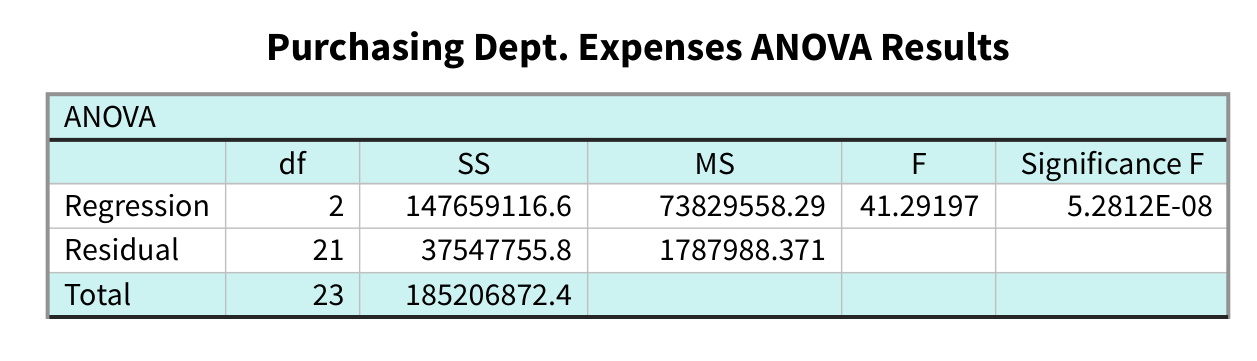
\includegraphics[width=0.95\textwidth,height=0.75\textheight,keepaspectratio]{../textbookForPractice/Figures/Ch_08/ILLUSTRATION 8.29.png}
    \end{figure}
\end{frame}

\begin{frame}{ILLUSTRATION 8.30}

    \begin{figure}[h]
        \centering
        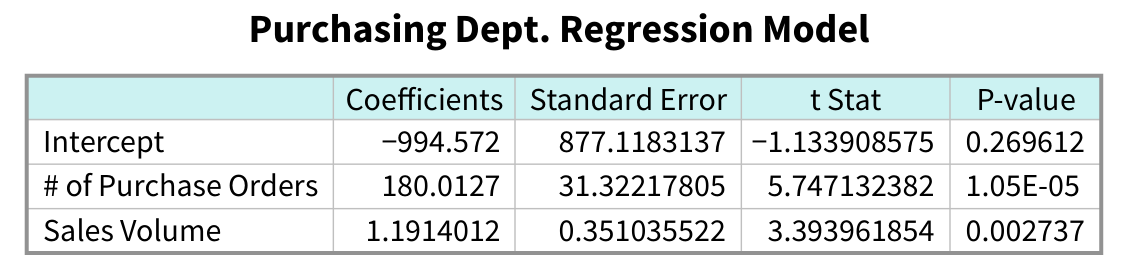
\includegraphics[width=0.95\textwidth,height=0.75\textheight,keepaspectratio]{../textbookForPractice/Figures/Ch_08/ILLUSTRATION 8.30.png}
    \end{figure}
\end{frame}

\begin{frame}{ILLUSTRATION 8.31}

    \begin{figure}[h]
        \centering
        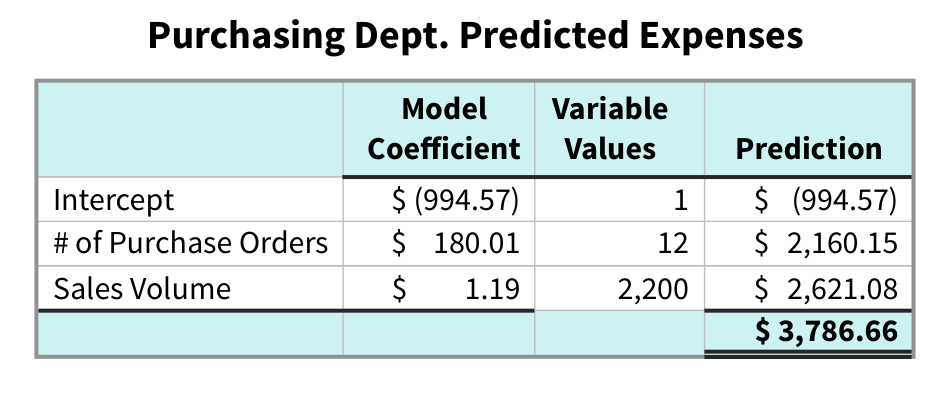
\includegraphics[width=0.95\textwidth,height=0.75\textheight,keepaspectratio]{../textbookForPractice/Figures/Ch_08/ILLUSTRATION 8.31.png}
    \end{figure}
\end{frame}

\begin{frame}{ILLUSTRATION 8.32}

    \begin{figure}[h]
        \centering
        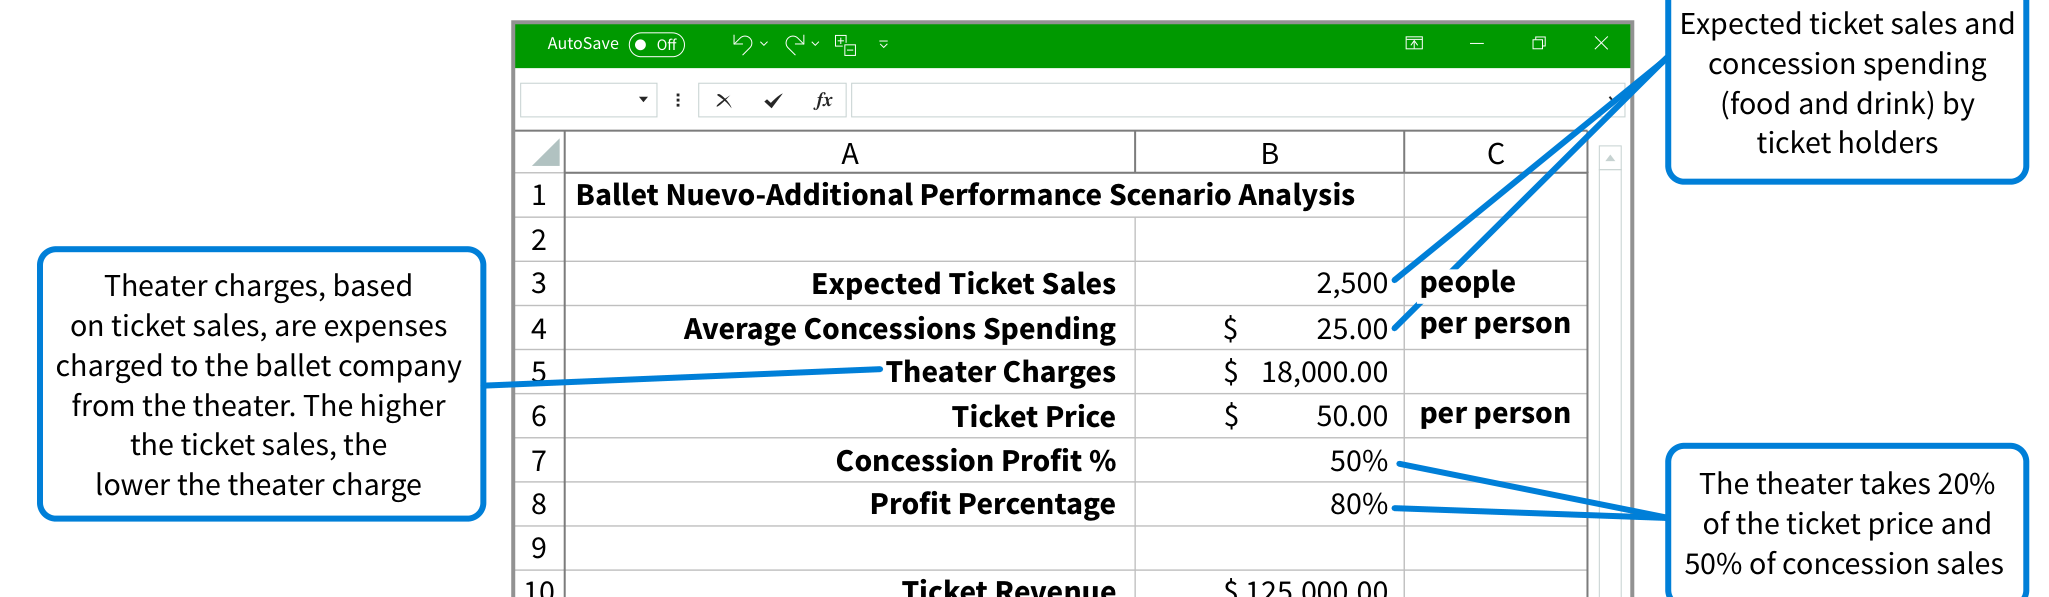
\includegraphics[width=0.95\textwidth,height=0.75\textheight,keepaspectratio]{../textbookForPractice/Figures/Ch_08/ILLUSTRATION 8.32.png}
    \end{figure}
\end{frame}

\begin{frame}{8.5 Đánh giá Phân tích Dự đoán và Đề xuất}
\begin{itemize}
    \item \textbf{Phân tích Dự đoán (Predictive):} Sử dụng mô hình (như Hồi quy - Regression) để dự báo tương lai.
    \item \textbf{Đánh giá Mô hình:}
    \begin{itemize}
        \item Hệ số $R^2$ có đủ cao không?
        \item Mối quan hệ có ý nghĩa thống kê (p-value < 0.05) không?
        \item Cẩn thận với "Tương quan không có nghĩa là Nhân quả" (Correlation vs. Causation).
    \end{itemize}
\end{itemize}
\end{frame}

\begin{frame}{ILLUSTRATION 8.32\_1}

    \begin{figure}[h]
        \centering
        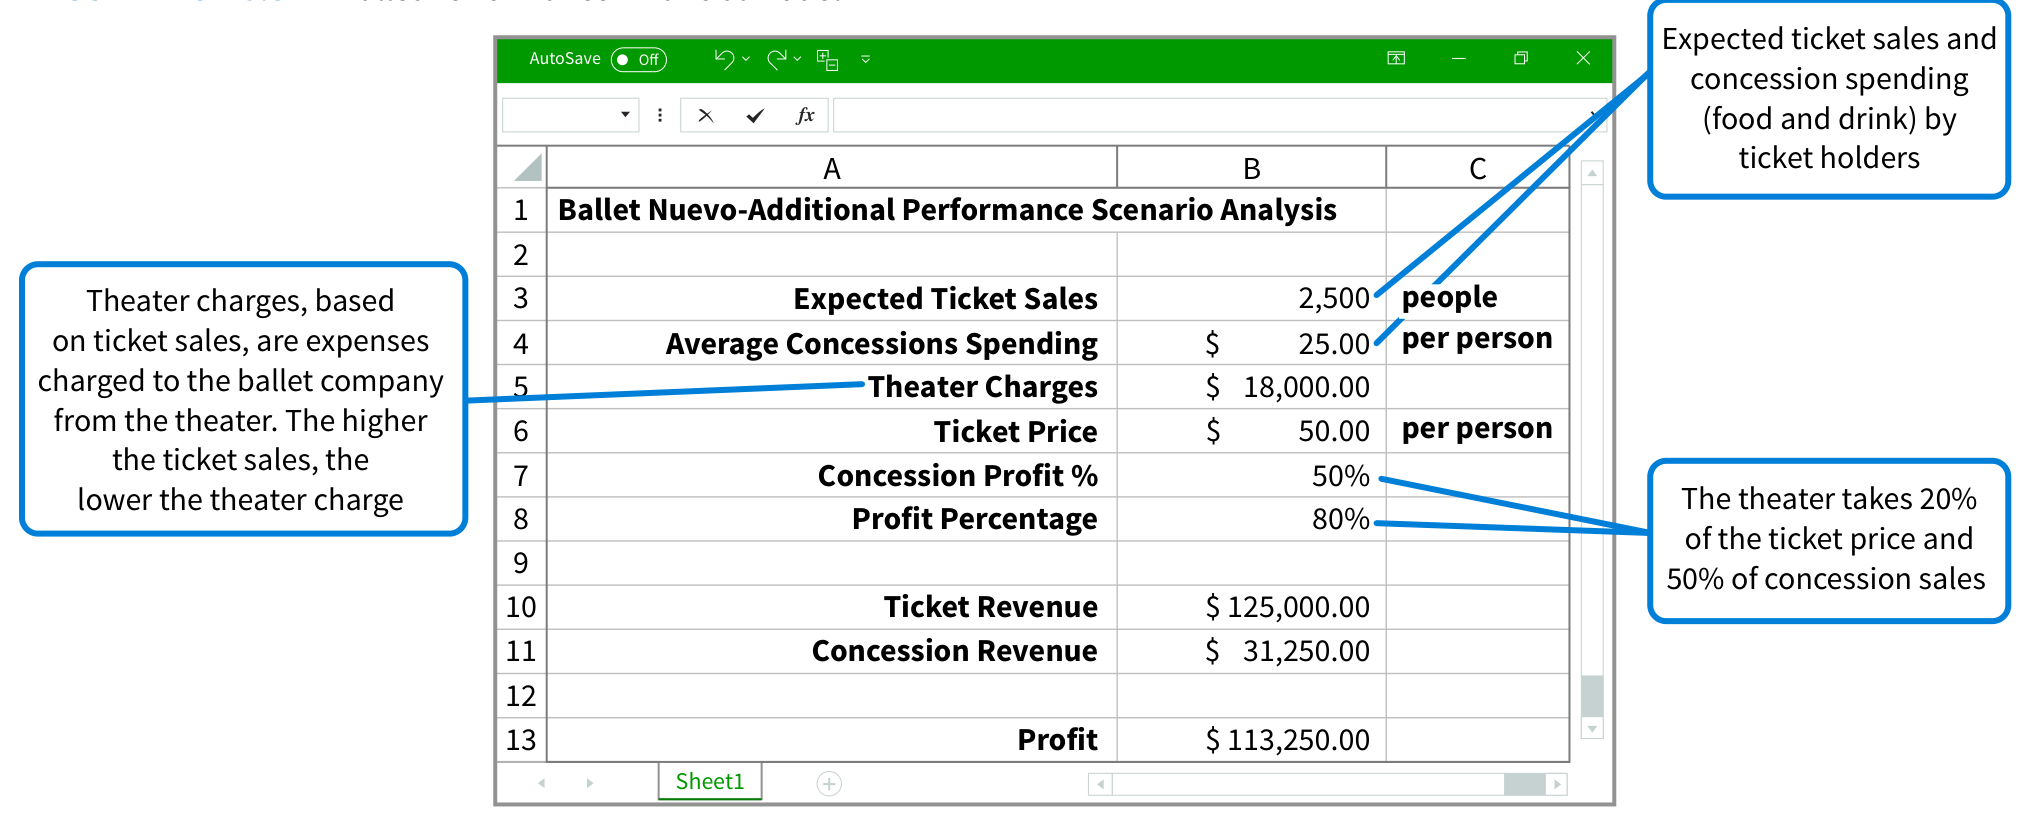
\includegraphics[width=0.95\textwidth,height=0.75\textheight,keepaspectratio]{../textbookForPractice/Figures/Ch_08/ILLUSTRATION 8.32_1.png}
    \end{figure}
\end{frame}

\begin{frame}{ILLUSTRATION 8.33}

    \begin{figure}[h]
        \centering
        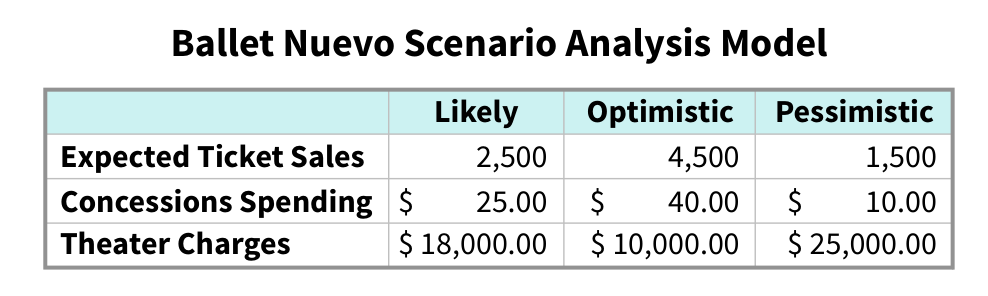
\includegraphics[width=0.95\textwidth,height=0.75\textheight,keepaspectratio]{../textbookForPractice/Figures/Ch_08/ILLUSTRATION 8.33.png}
    \end{figure}
\end{frame}

\begin{frame}{ILLUSTRATION 8.34}

    \begin{figure}[h]
        \centering
        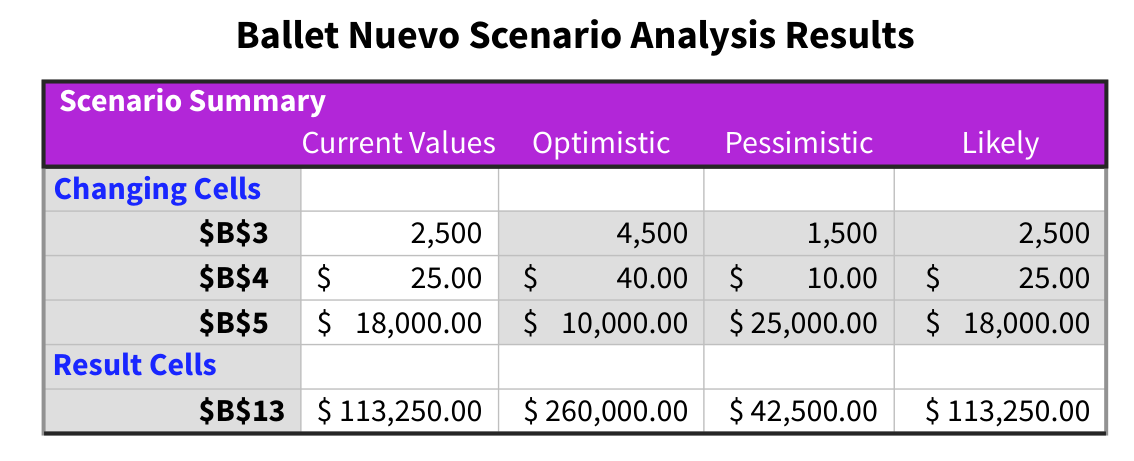
\includegraphics[width=0.95\textwidth,height=0.75\textheight,keepaspectratio]{../textbookForPractice/Figures/Ch_08/ILLUSTRATION 8.34.png}
    \end{figure}
\end{frame}

\begin{frame}{ILLUSTRATION 8.35}

    \begin{figure}[h]
        \centering
        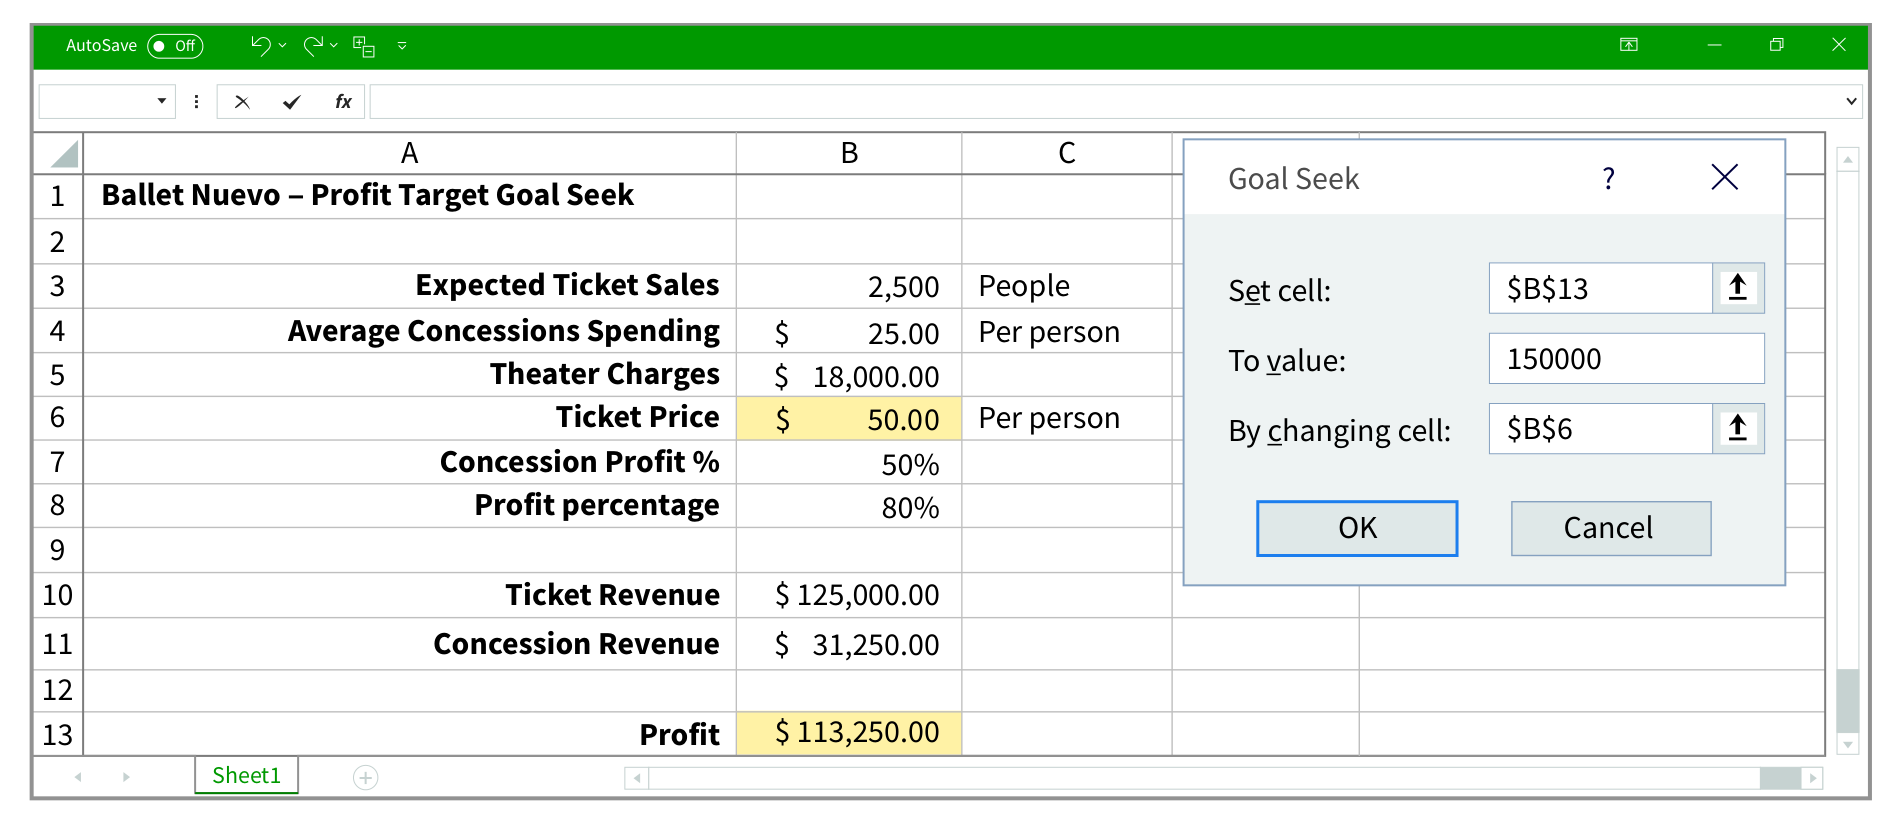
\includegraphics[width=0.95\textwidth,height=0.75\textheight,keepaspectratio]{../textbookForPractice/Figures/Ch_08/ILLUSTRATION 8.35.png}
    \end{figure}
\end{frame}

\begin{frame}{ILLUSTRATION 8.36}

    \begin{figure}[h]
        \centering
        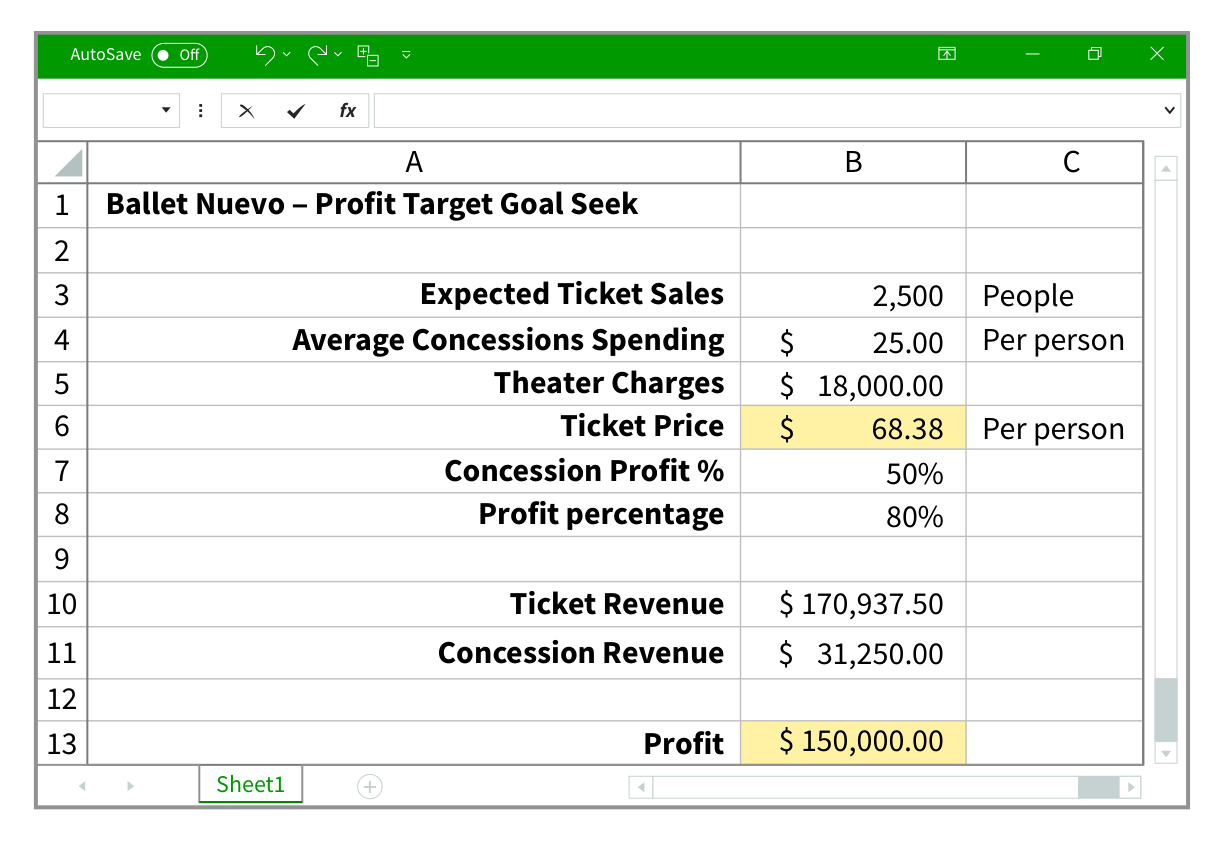
\includegraphics[width=0.95\textwidth,height=0.75\textheight,keepaspectratio]{../textbookForPractice/Figures/Ch_08/ILLUSTRATION 8.36.png}
    \end{figure}
\end{frame}

\begin{frame}{ILLUSTRATION 8.37}

    \begin{figure}[h]
        \centering
        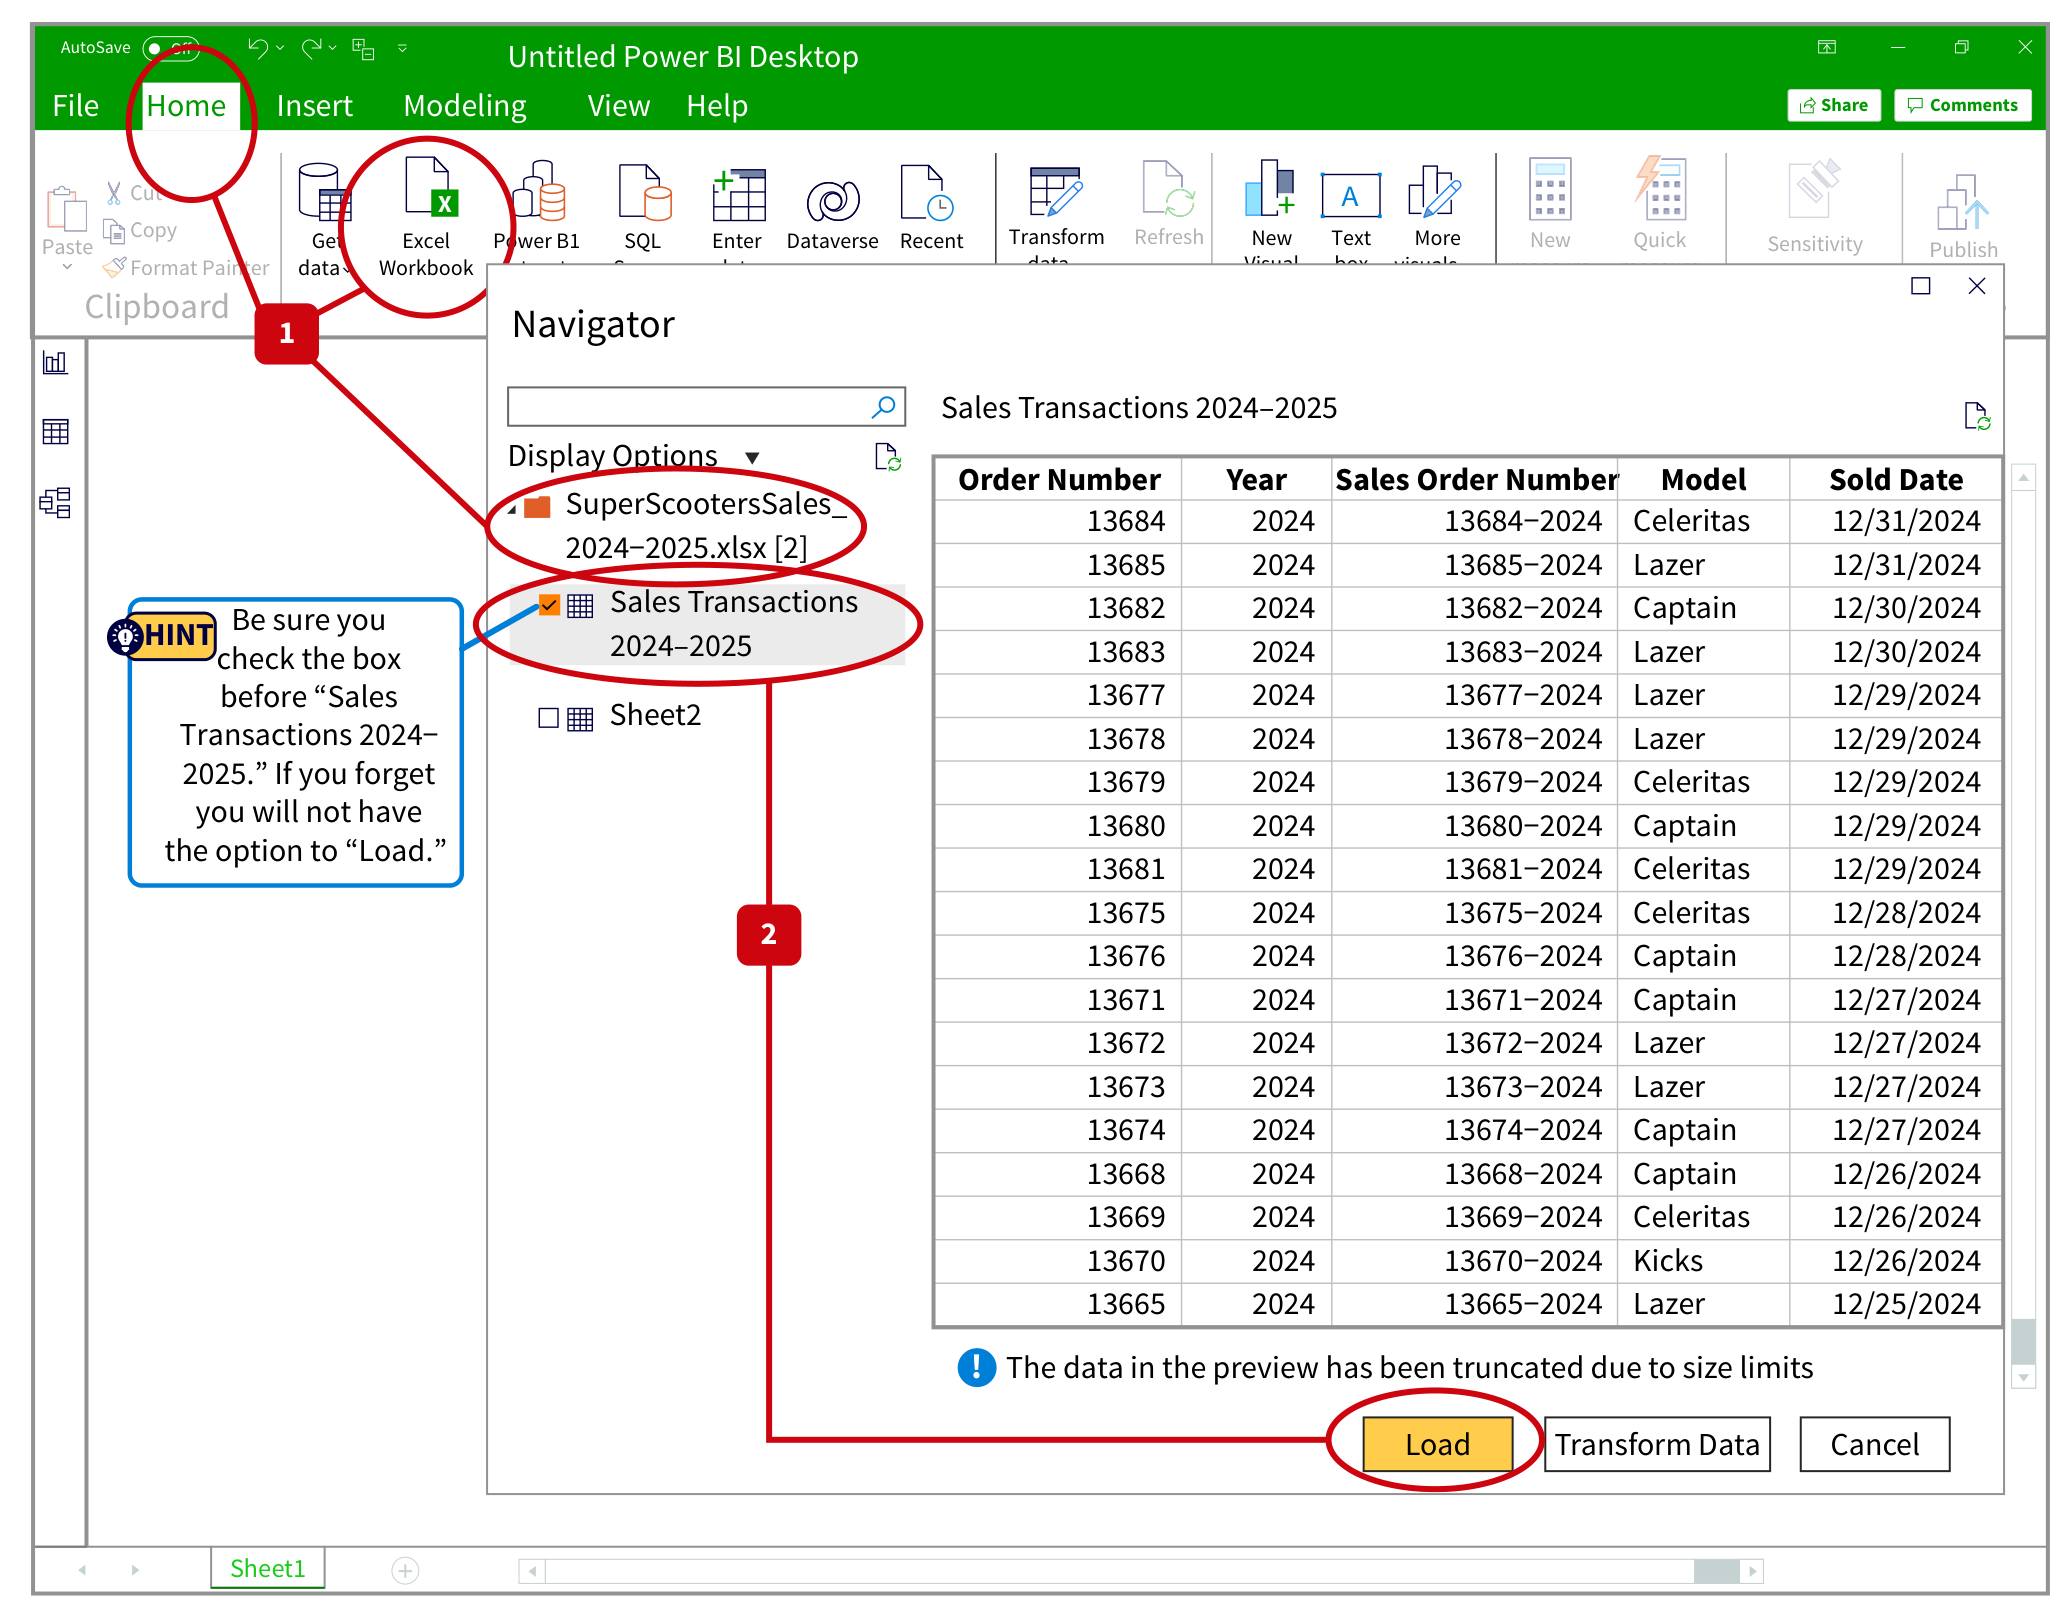
\includegraphics[width=0.95\textwidth,height=0.75\textheight,keepaspectratio]{../textbookForPractice/Figures/Ch_08/ILLUSTRATION 8.37.png}
    \end{figure}
\end{frame}

\begin{frame}{Đánh giá Phân tích Đề xuất}
\begin{itemize}
    \item \textbf{Phân tích Đề xuất (Prescriptive):} Tối ưu hóa các nguồn lực để đạt kết quả tốt nhất.
    \item \textbf{Đánh giá Khả năng Thực thi:} Đề xuất của AI có khả thi trong điều kiện ngân sách và chính sách của công ty không?
    \item \textbf{Kết luận:} Con người luôn là chốt chặn cuối cùng trong quá trình ra quyết định tài chính.
\end{itemize}
\end{frame}

\begin{frame}{ILLUSTRATION 8.38}

    \begin{figure}[h]
        \centering
        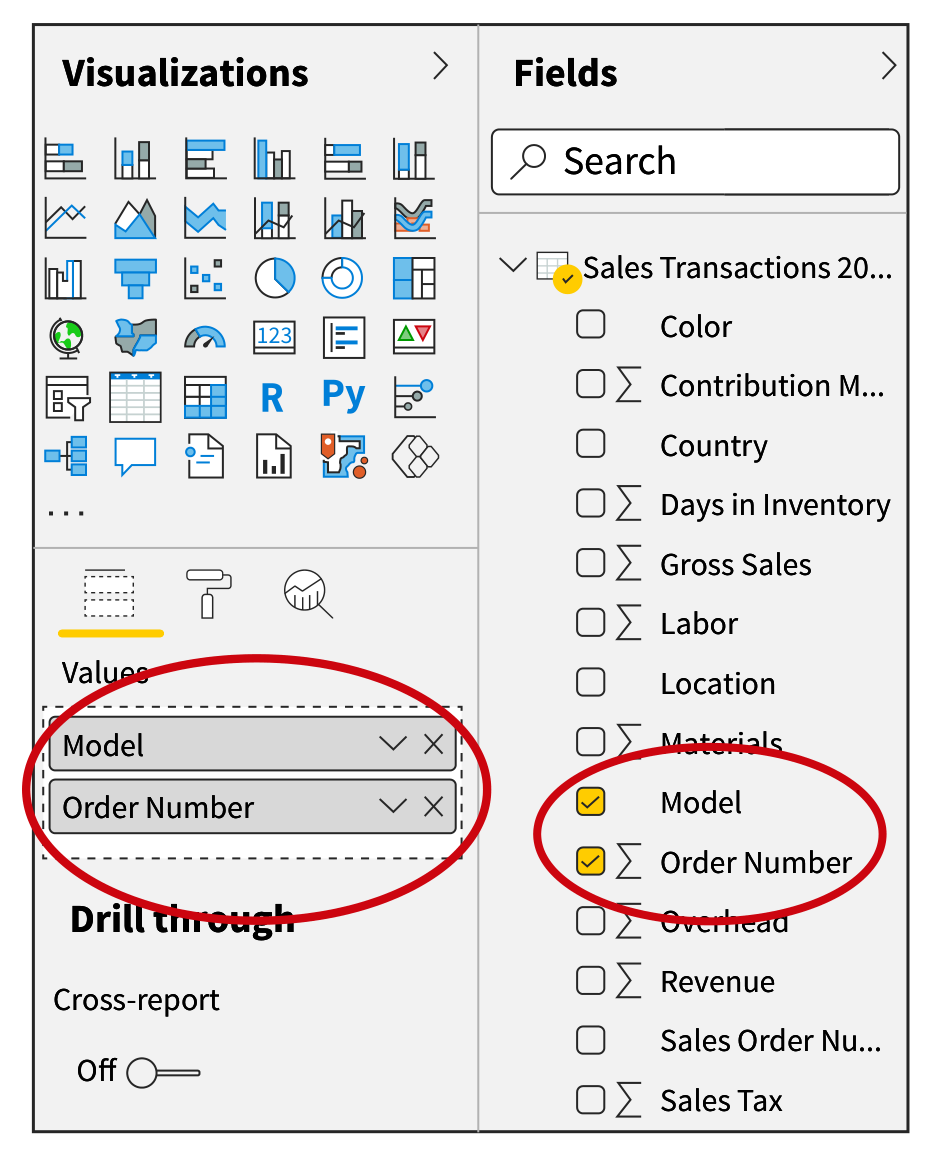
\includegraphics[width=0.95\textwidth,height=0.75\textheight,keepaspectratio]{../textbookForPractice/Figures/Ch_08/ILLUSTRATION 8.38.png}
    \end{figure}
\end{frame}

\begin{frame}{ILLUSTRATION 8.39}

    \begin{figure}[h]
        \centering
        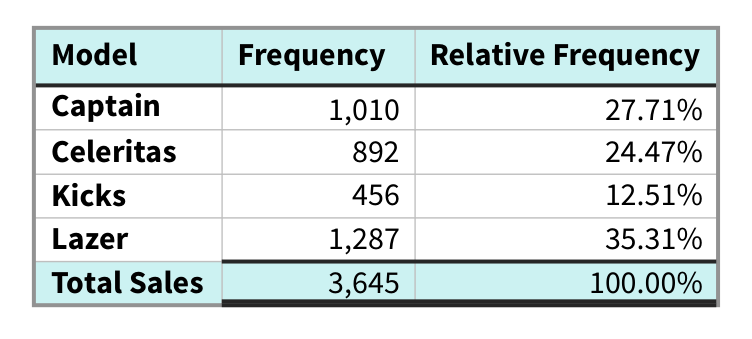
\includegraphics[width=0.95\textwidth,height=0.75\textheight,keepaspectratio]{../textbookForPractice/Figures/Ch_08/ILLUSTRATION 8.39.png}
    \end{figure}
\end{frame}

\begin{frame}{ILLUSTRATION 8.40}

    \begin{figure}[h]
        \centering
        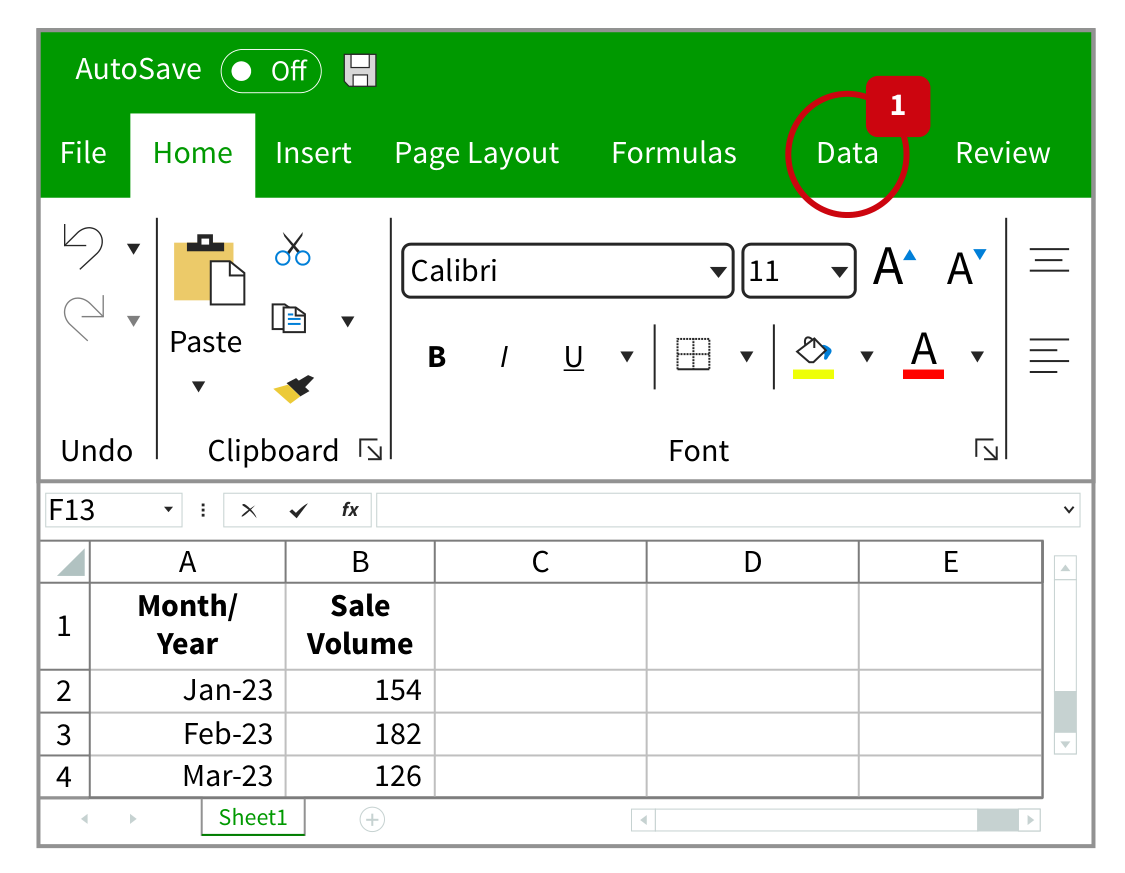
\includegraphics[width=0.95\textwidth,height=0.75\textheight,keepaspectratio]{../textbookForPractice/Figures/Ch_08/ILLUSTRATION 8.40.png}
    \end{figure}
\end{frame}

\begin{frame}{ILLUSTRATION 8.41}

    \begin{figure}[h]
        \centering
        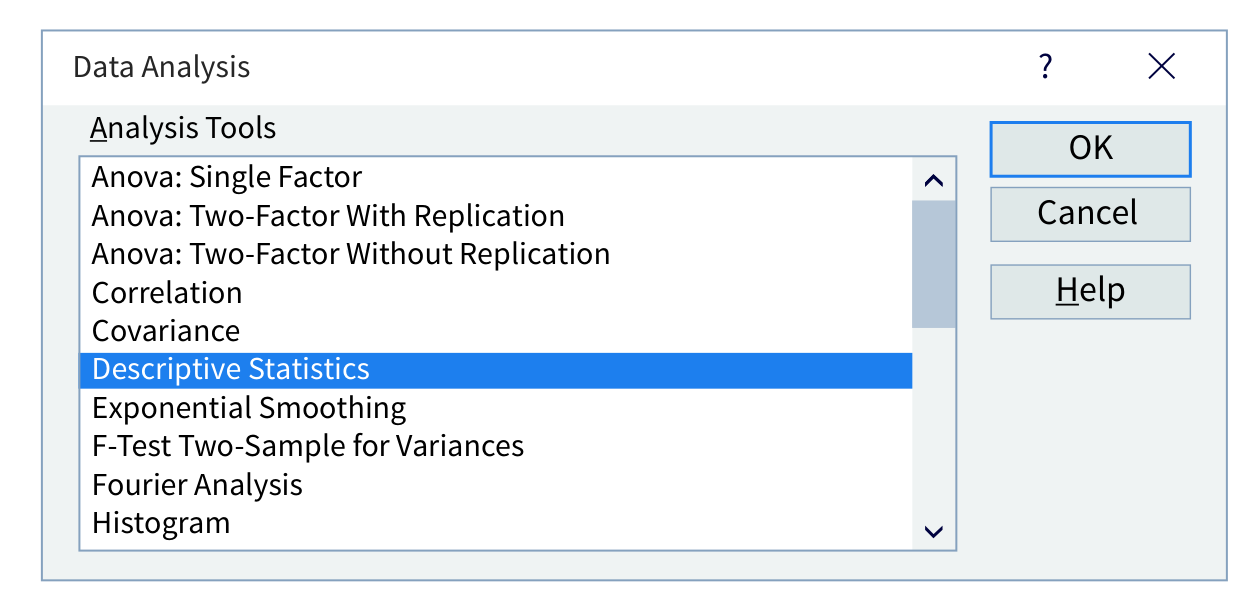
\includegraphics[width=0.95\textwidth,height=0.75\textheight,keepaspectratio]{../textbookForPractice/Figures/Ch_08/ILLUSTRATION 8.41.png}
    \end{figure}
\end{frame}

\begin{frame}{ILLUSTRATION 8.42}

    \begin{figure}[h]
        \centering
        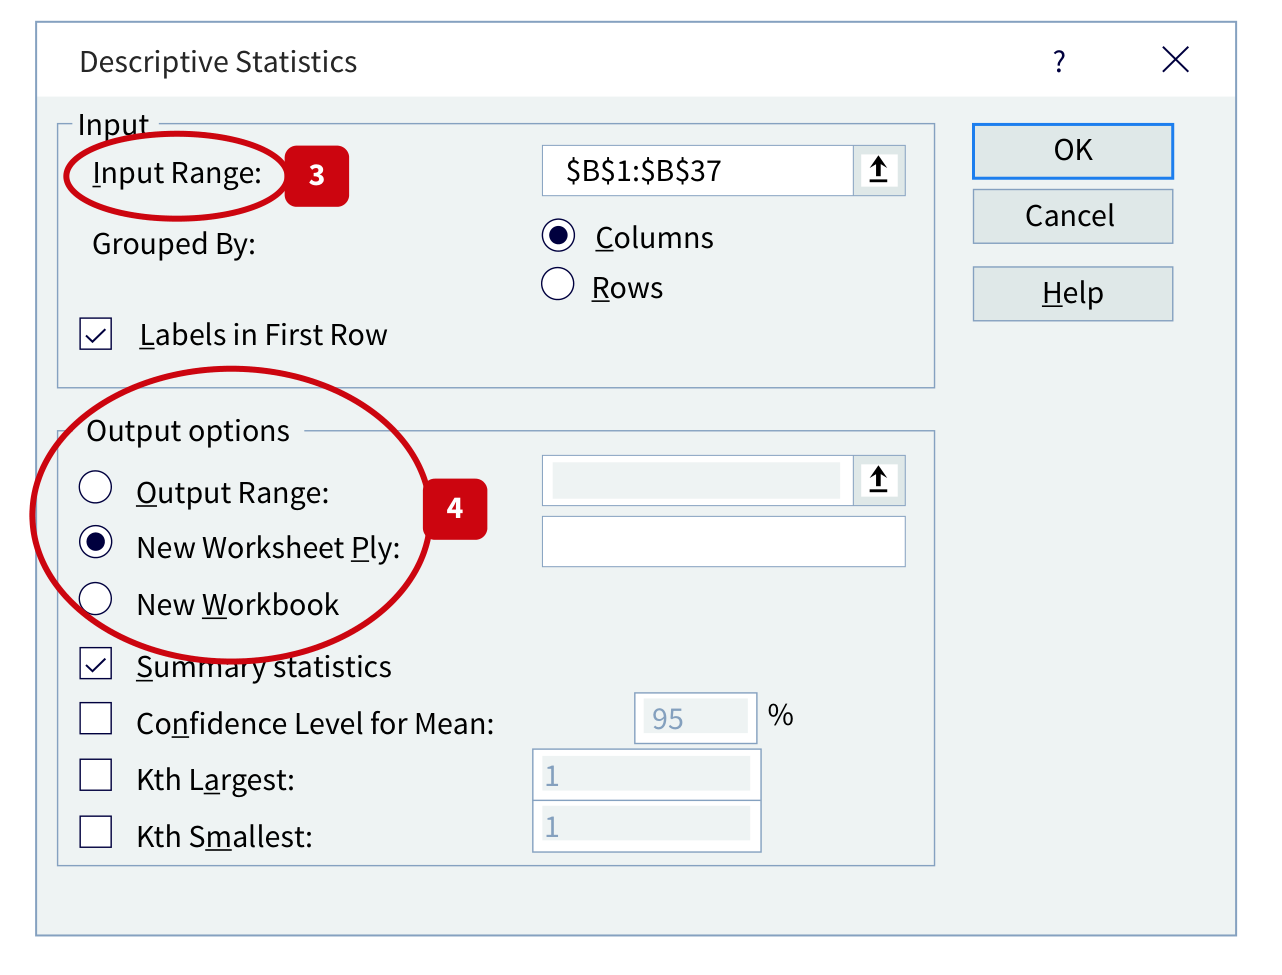
\includegraphics[width=0.95\textwidth,height=0.75\textheight,keepaspectratio]{../textbookForPractice/Figures/Ch_08/ILLUSTRATION 8.42.png}
    \end{figure}
\end{frame}

\begin{frame}{Bài tập Ngắn (Brief Exercises)}
\begin{center}
        \Huge \textbf{Phần Bài tập Ngắn} \\
        \vspace{0.5cm}
        \Large Brief Exercises (BE)
    \end{center}
\end{frame}

\begin{frame}{BE 8.3 \& BE 8.4}
    \begin{columns}
        \begin{column}{0.5\textwidth}
            \begin{figure}[h]
                \centering
                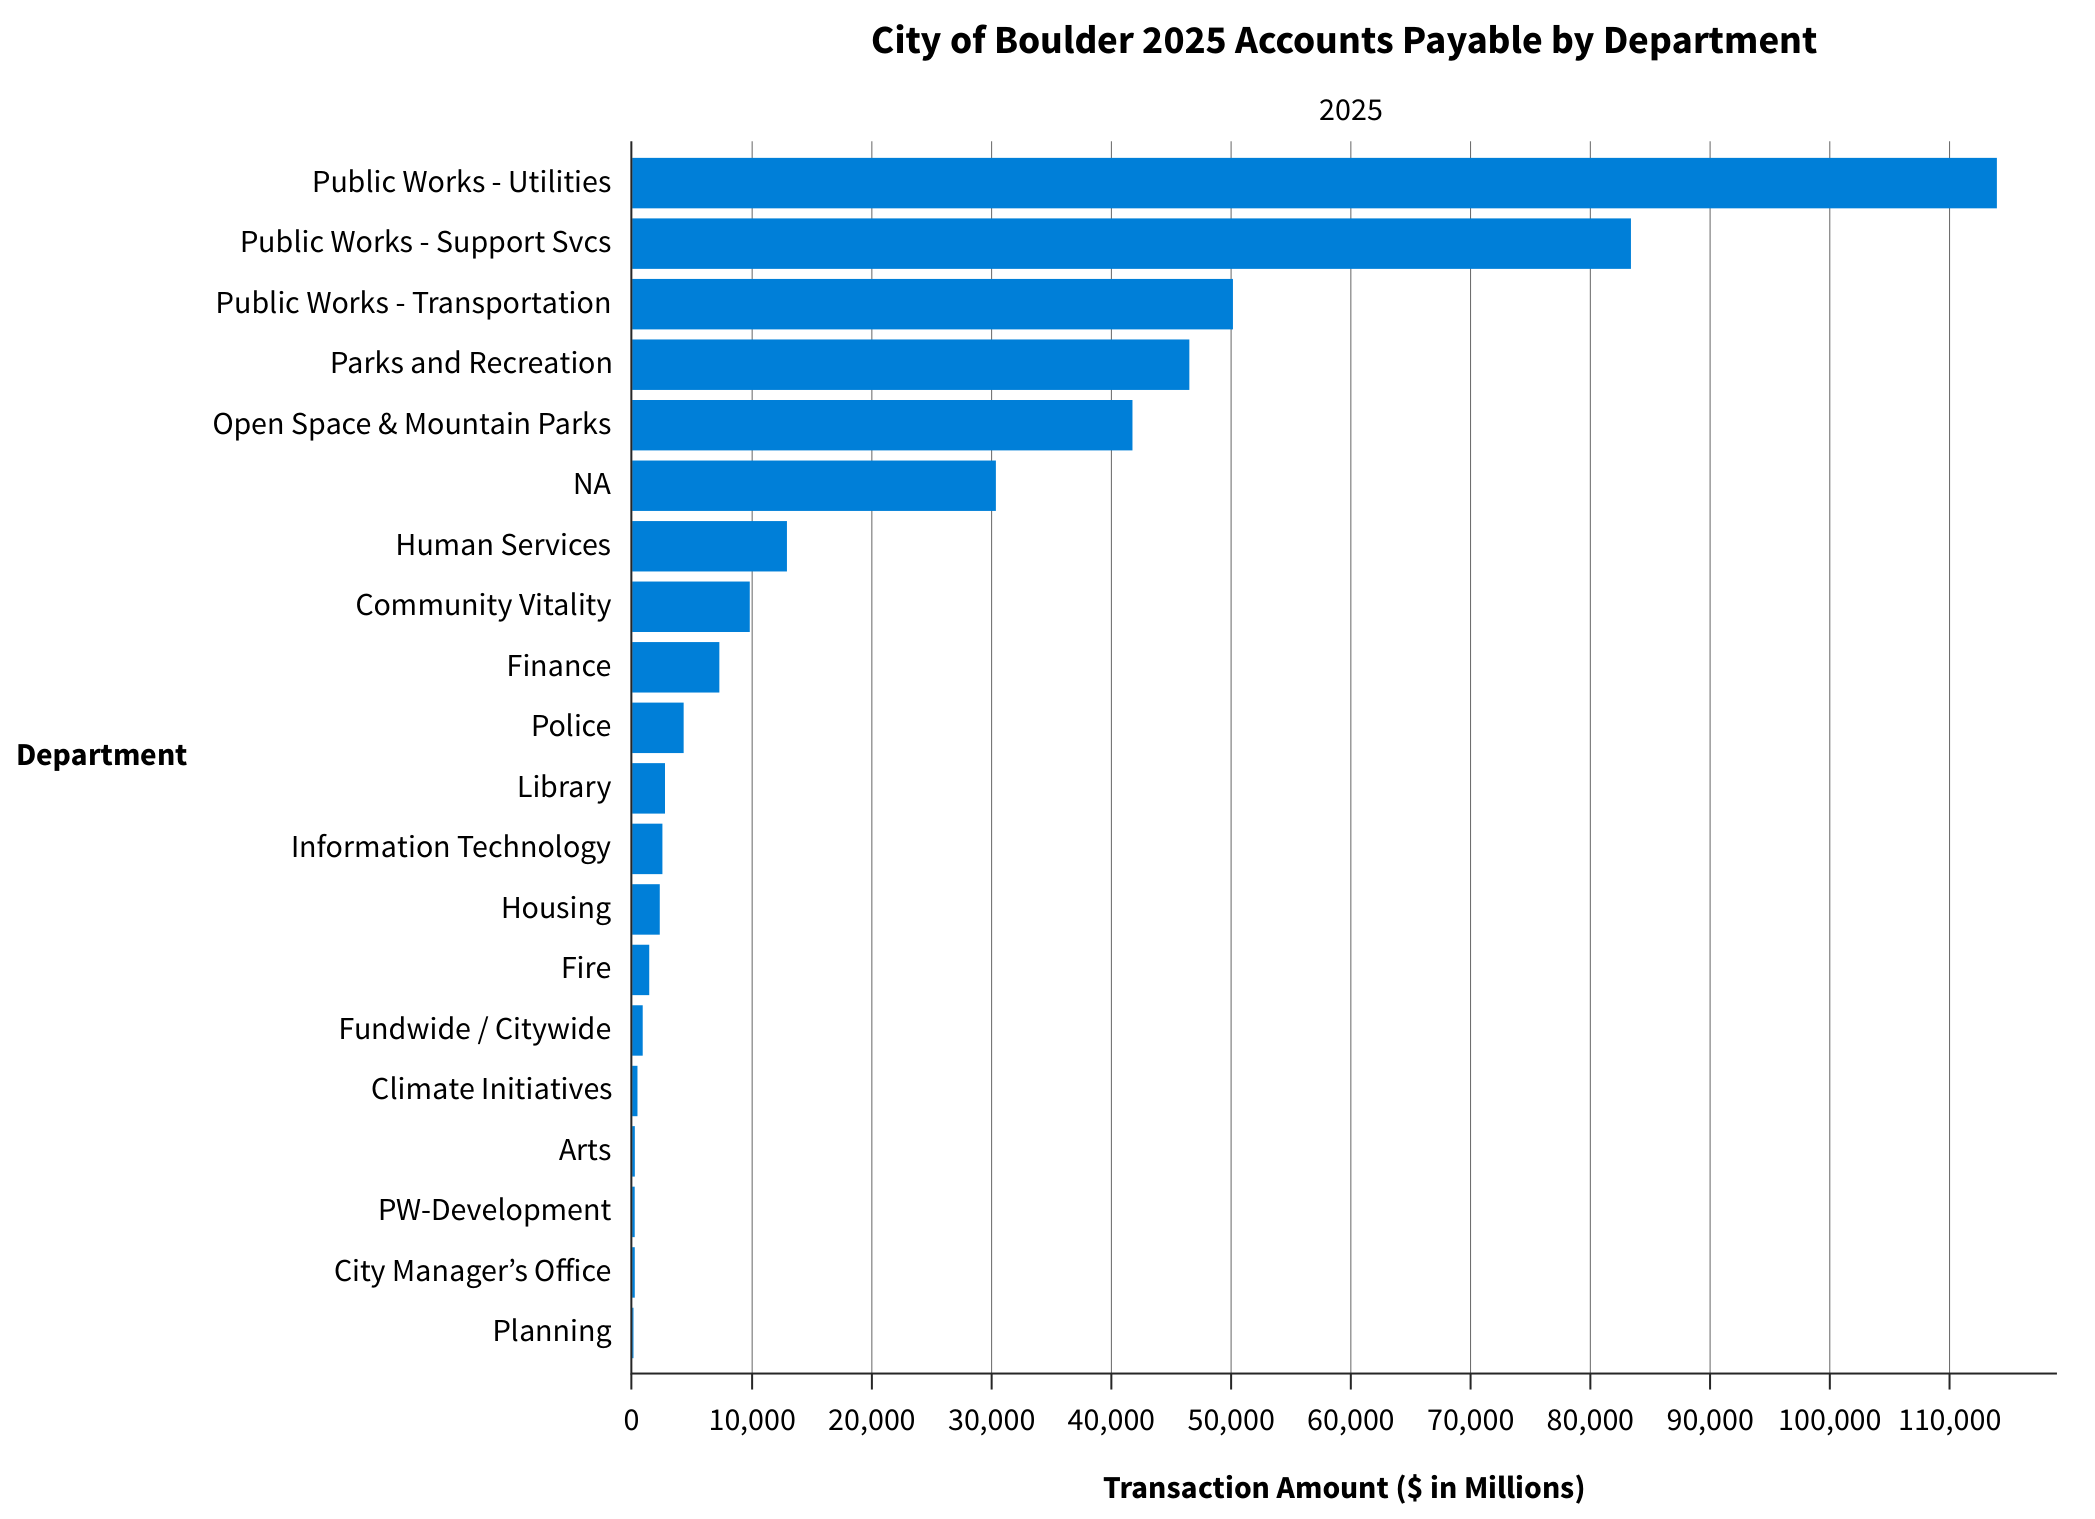
\includegraphics[width=\textwidth,height=0.7\textheight,keepaspectratio]{../textbookForPractice/Figures/Ch_08/BE 8.3.png}
            \end{figure}
        \end{column}
        \begin{column}{0.5\textwidth}
            \begin{figure}[h]
                \centering
                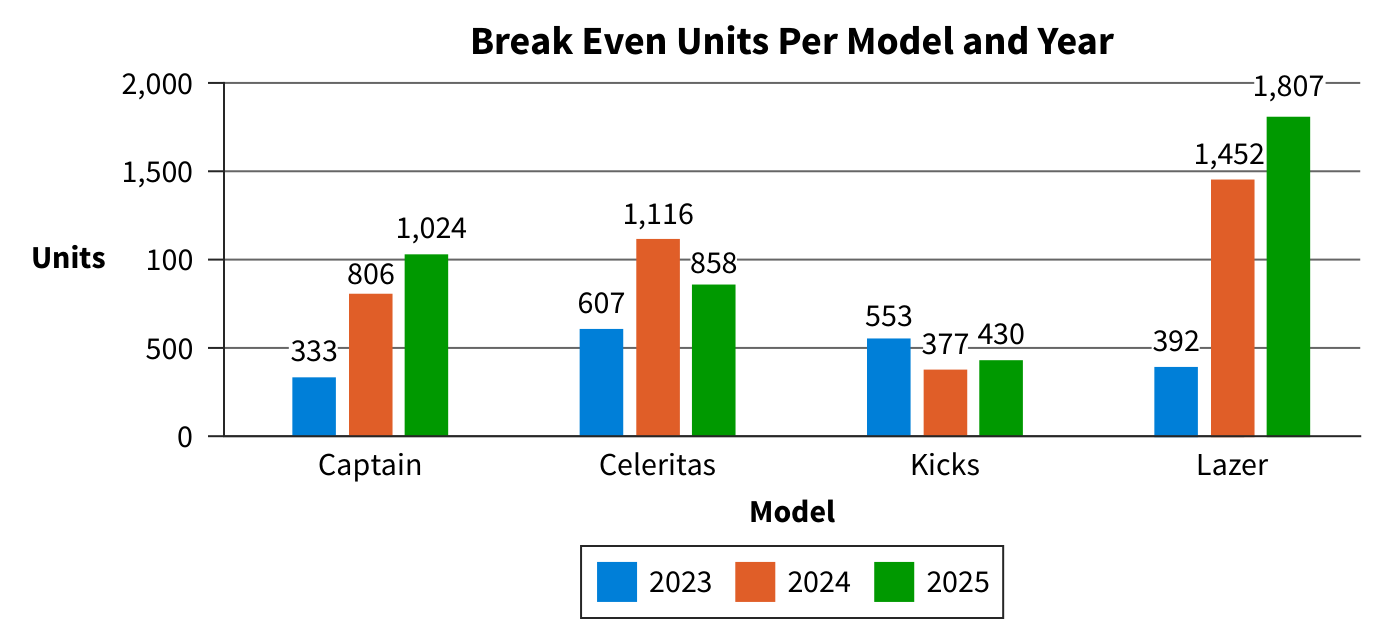
\includegraphics[width=\textwidth,height=0.7\textheight,keepaspectratio]{../textbookForPractice/Figures/Ch_08/BE 8.4.png}
            \end{figure}
        \end{column}
    \end{columns}
\end{frame}

\begin{frame}{BE 8.7 \& BE 8.8}
    \begin{columns}
        \begin{column}{0.5\textwidth}
            \begin{figure}[h]
                \centering
                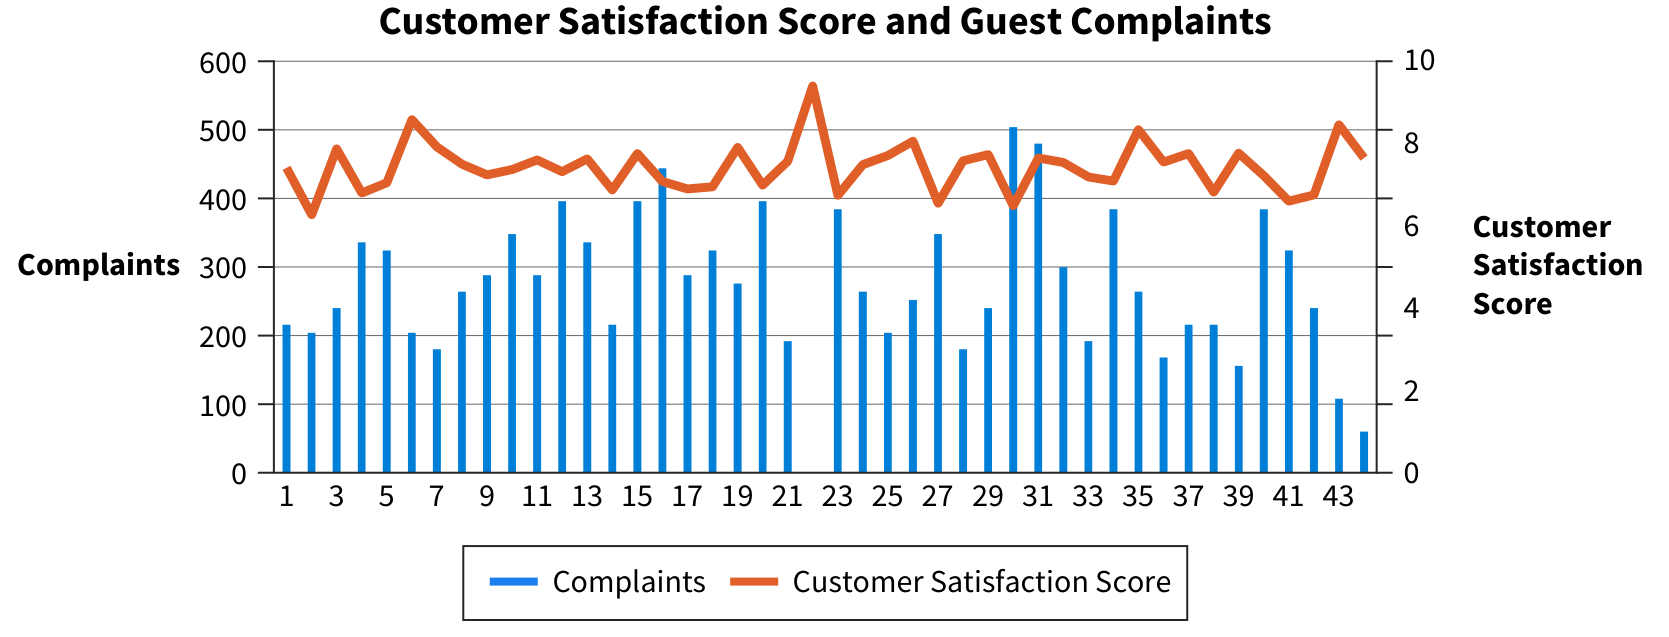
\includegraphics[width=\textwidth,height=0.7\textheight,keepaspectratio]{../textbookForPractice/Figures/Ch_08/BE 8.7.png}
            \end{figure}
        \end{column}
        \begin{column}{0.5\textwidth}
            \begin{figure}[h]
                \centering
                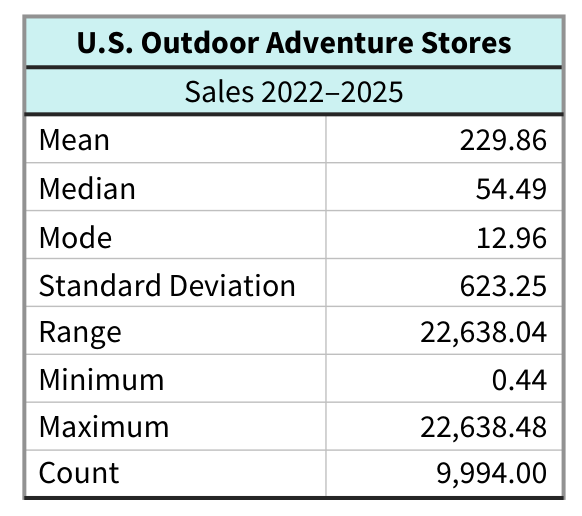
\includegraphics[width=\textwidth,height=0.7\textheight,keepaspectratio]{../textbookForPractice/Figures/Ch_08/BE 8.8.png}
            \end{figure}
        \end{column}
    \end{columns}
\end{frame}

\begin{frame}{BE 8.9 \& BE 8.10}
    \begin{columns}
        \begin{column}{0.5\textwidth}
            \begin{figure}[h]
                \centering
                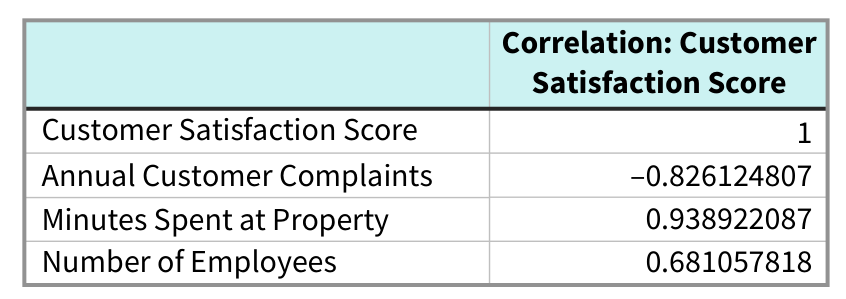
\includegraphics[width=\textwidth,height=0.7\textheight,keepaspectratio]{../textbookForPractice/Figures/Ch_08/BE 8.9.png}
            \end{figure}
        \end{column}
        \begin{column}{0.5\textwidth}
            \begin{figure}[h]
                \centering
                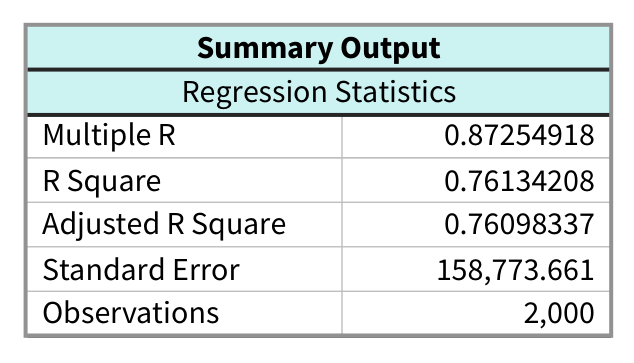
\includegraphics[width=\textwidth,height=0.7\textheight,keepaspectratio]{../textbookForPractice/Figures/Ch_08/BE 8.10.png}
            \end{figure}
        \end{column}
    \end{columns}
\end{frame}

\begin{frame}{BE 8.11}

    \begin{figure}[h]
        \centering
        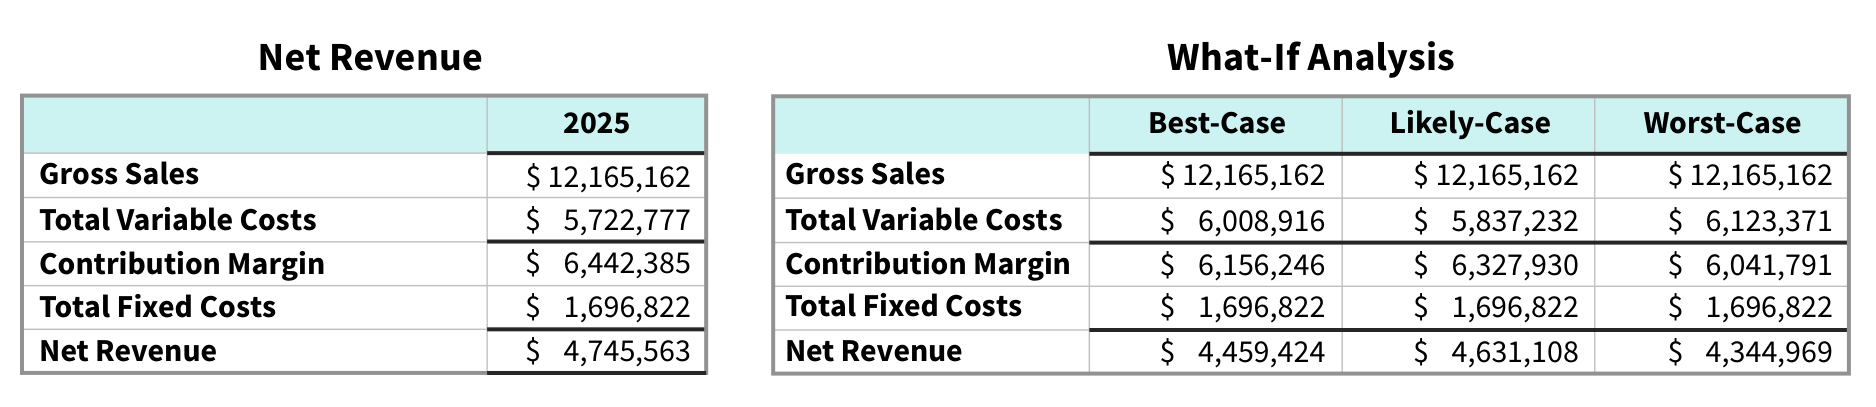
\includegraphics[width=0.95\textwidth,height=0.75\textheight,keepaspectratio]{../textbookForPractice/Figures/Ch_08/BE 8.11.png}
    \end{figure}
\end{frame}

\begin{frame}{Bài tập (Exercises)}
\begin{center}
        \Huge \textbf{Phần Bài tập} \\
        \vspace{0.5cm}
        \Large Exercises (EX)
    \end{center}
\end{frame}

\begin{frame}{EX 8.1 \& EX 8.2}
    \begin{columns}
        \begin{column}{0.5\textwidth}
            \begin{figure}[h]
                \centering
                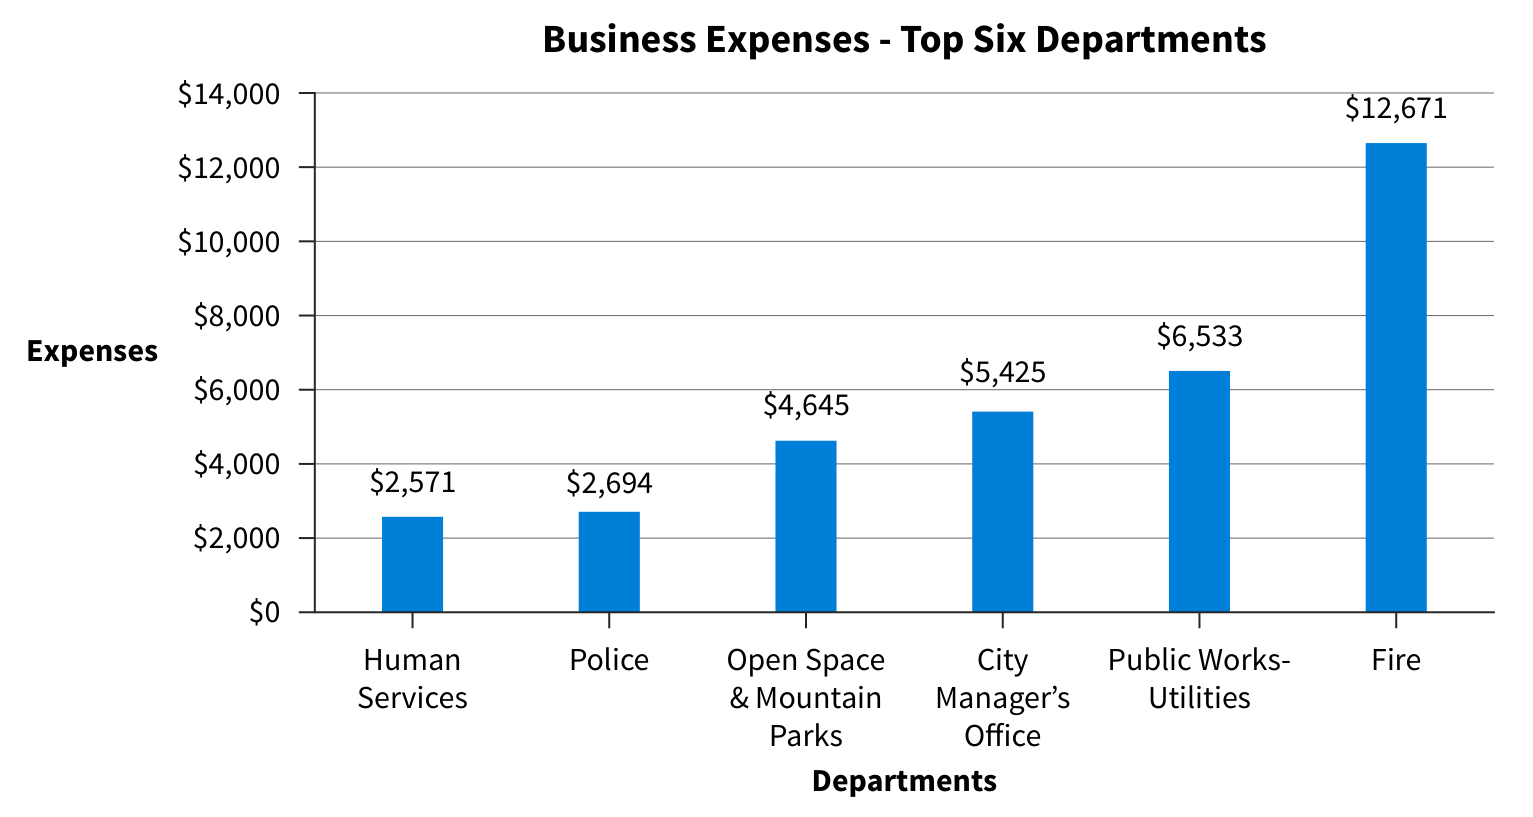
\includegraphics[width=\textwidth,height=0.7\textheight,keepaspectratio]{../textbookForPractice/Figures/Ch_08/EX 8.1.png}
            \end{figure}
        \end{column}
        \begin{column}{0.5\textwidth}
            \begin{figure}[h]
                \centering
                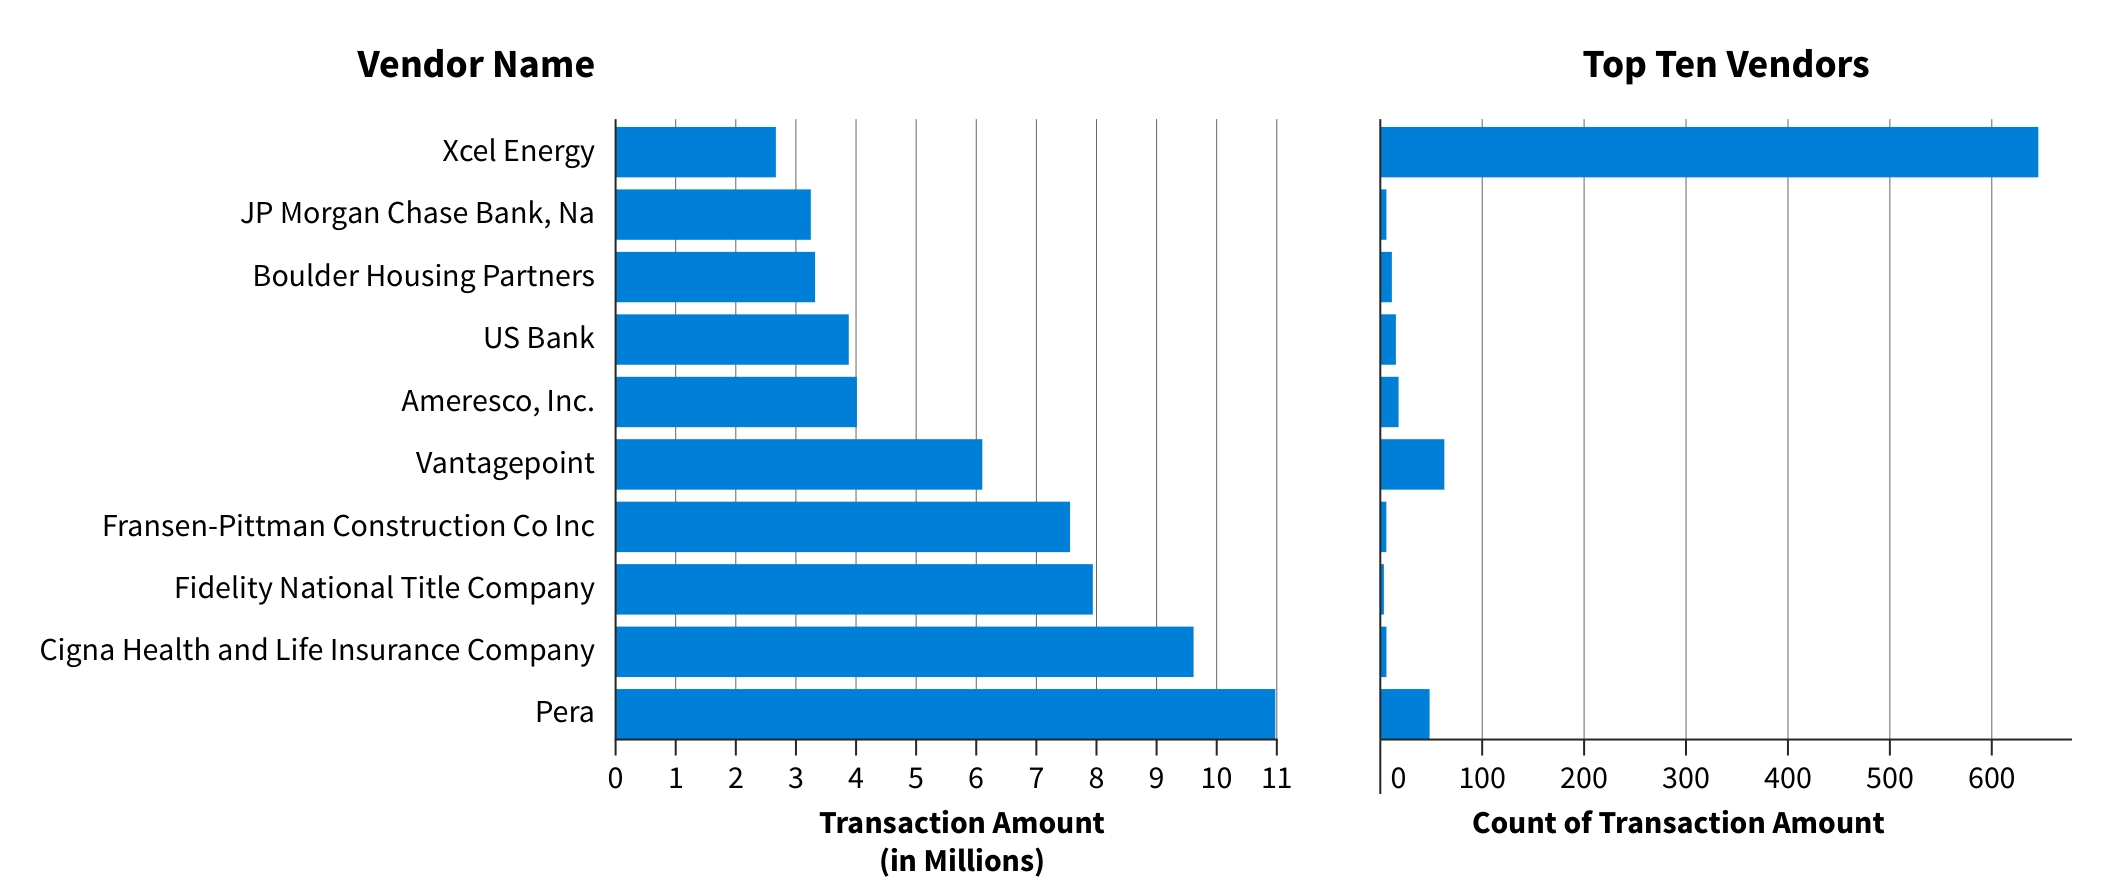
\includegraphics[width=\textwidth,height=0.7\textheight,keepaspectratio]{../textbookForPractice/Figures/Ch_08/EX 8.2.png}
            \end{figure}
        \end{column}
    \end{columns}
\end{frame}

\begin{frame}{EX 8.4 \& EX 8.5}
    \begin{columns}
        \begin{column}{0.5\textwidth}
            \begin{figure}[h]
                \centering
                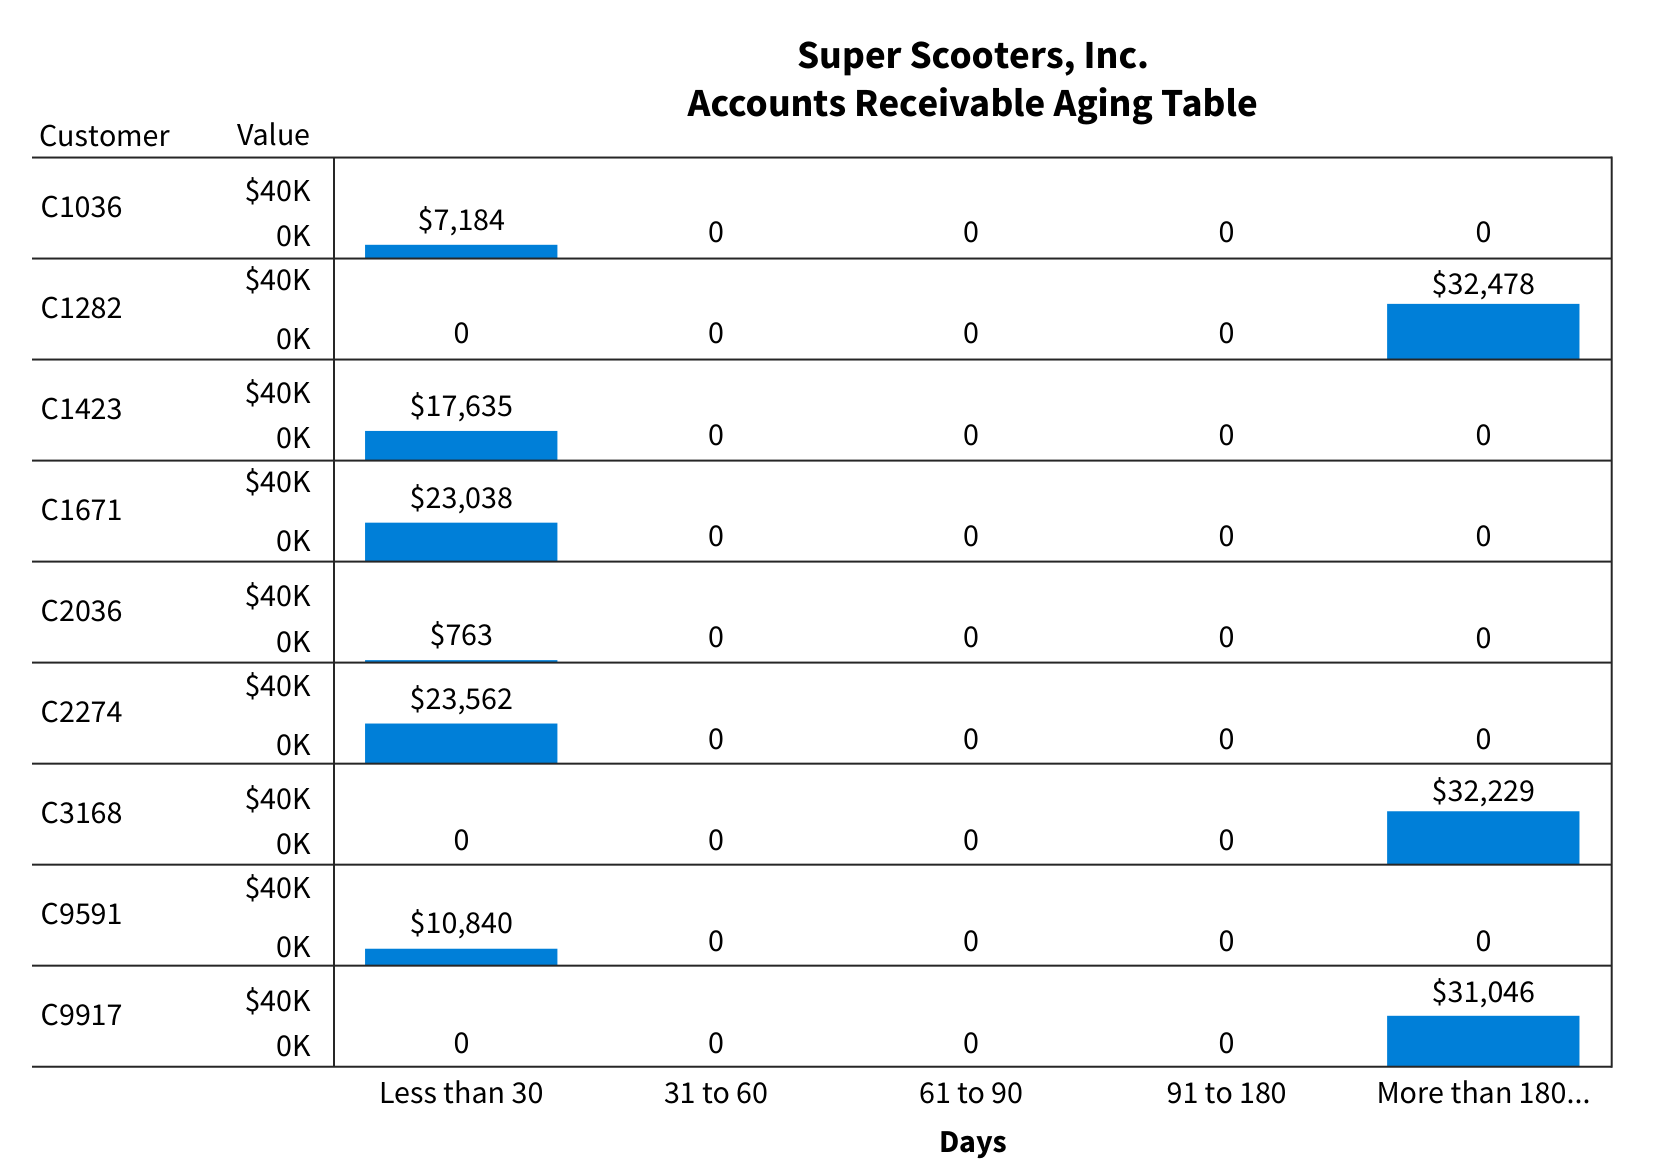
\includegraphics[width=\textwidth,height=0.7\textheight,keepaspectratio]{../textbookForPractice/Figures/Ch_08/EX 8.4.png}
            \end{figure}
        \end{column}
        \begin{column}{0.5\textwidth}
            \begin{figure}[h]
                \centering
                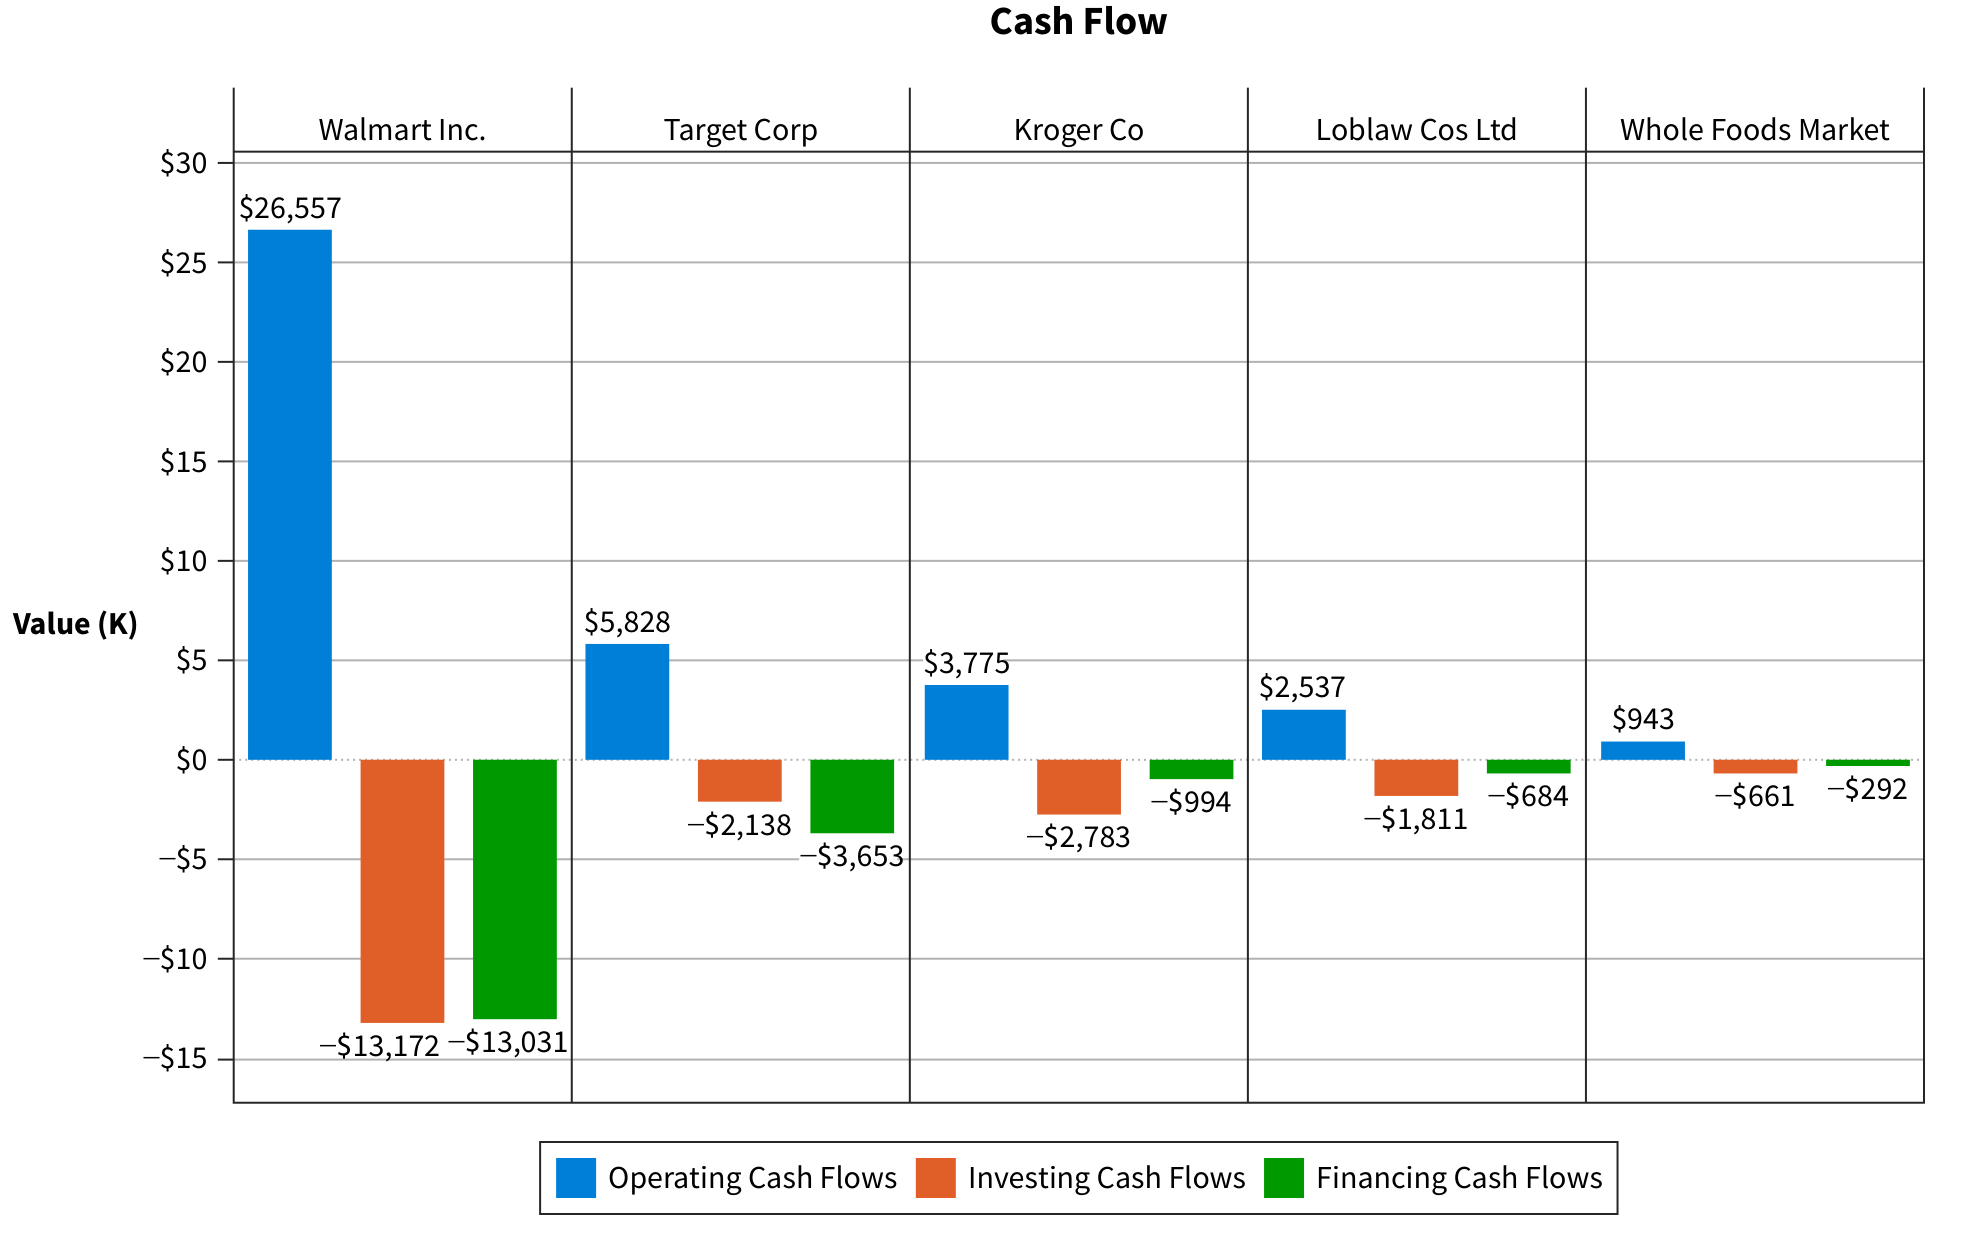
\includegraphics[width=\textwidth,height=0.7\textheight,keepaspectratio]{../textbookForPractice/Figures/Ch_08/EX 8.5.png}
            \end{figure}
        \end{column}
    \end{columns}
\end{frame}

\begin{frame}{EX 8.6 \& EX 8.7}
    \begin{columns}
        \begin{column}{0.5\textwidth}
            \begin{figure}[h]
                \centering
                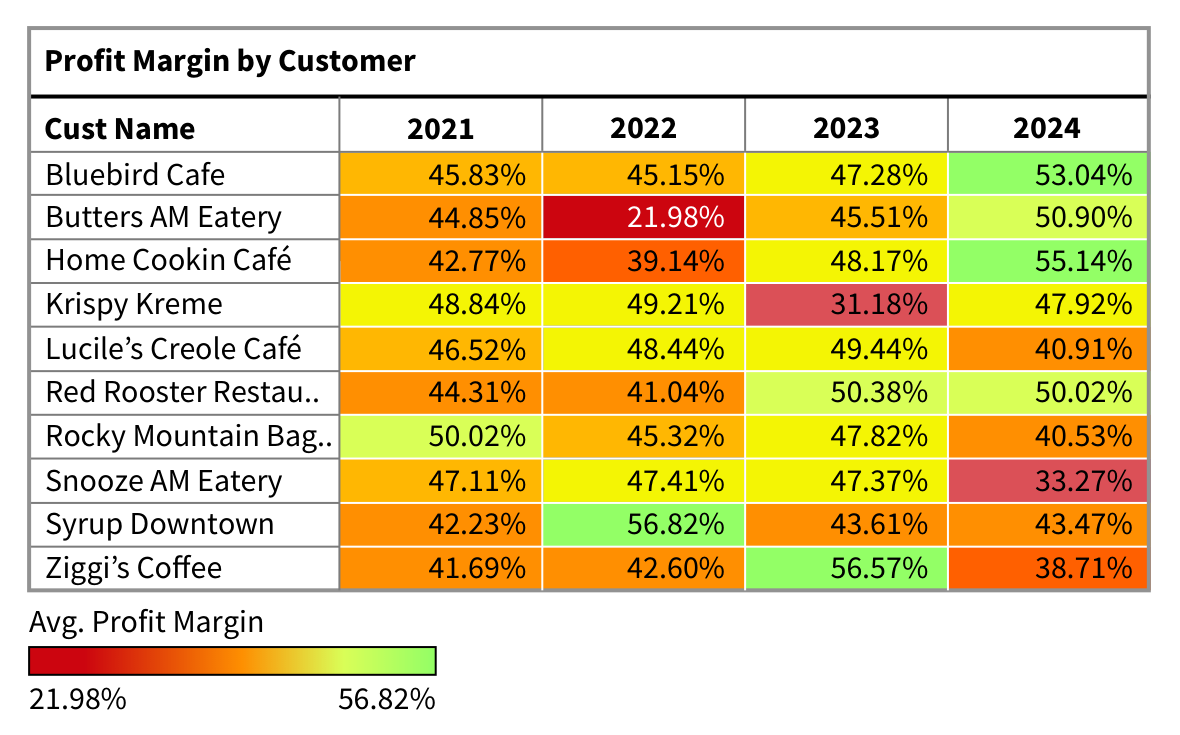
\includegraphics[width=\textwidth,height=0.7\textheight,keepaspectratio]{../textbookForPractice/Figures/Ch_08/EX 8.6.png}
            \end{figure}
        \end{column}
        \begin{column}{0.5\textwidth}
            \begin{figure}[h]
                \centering
                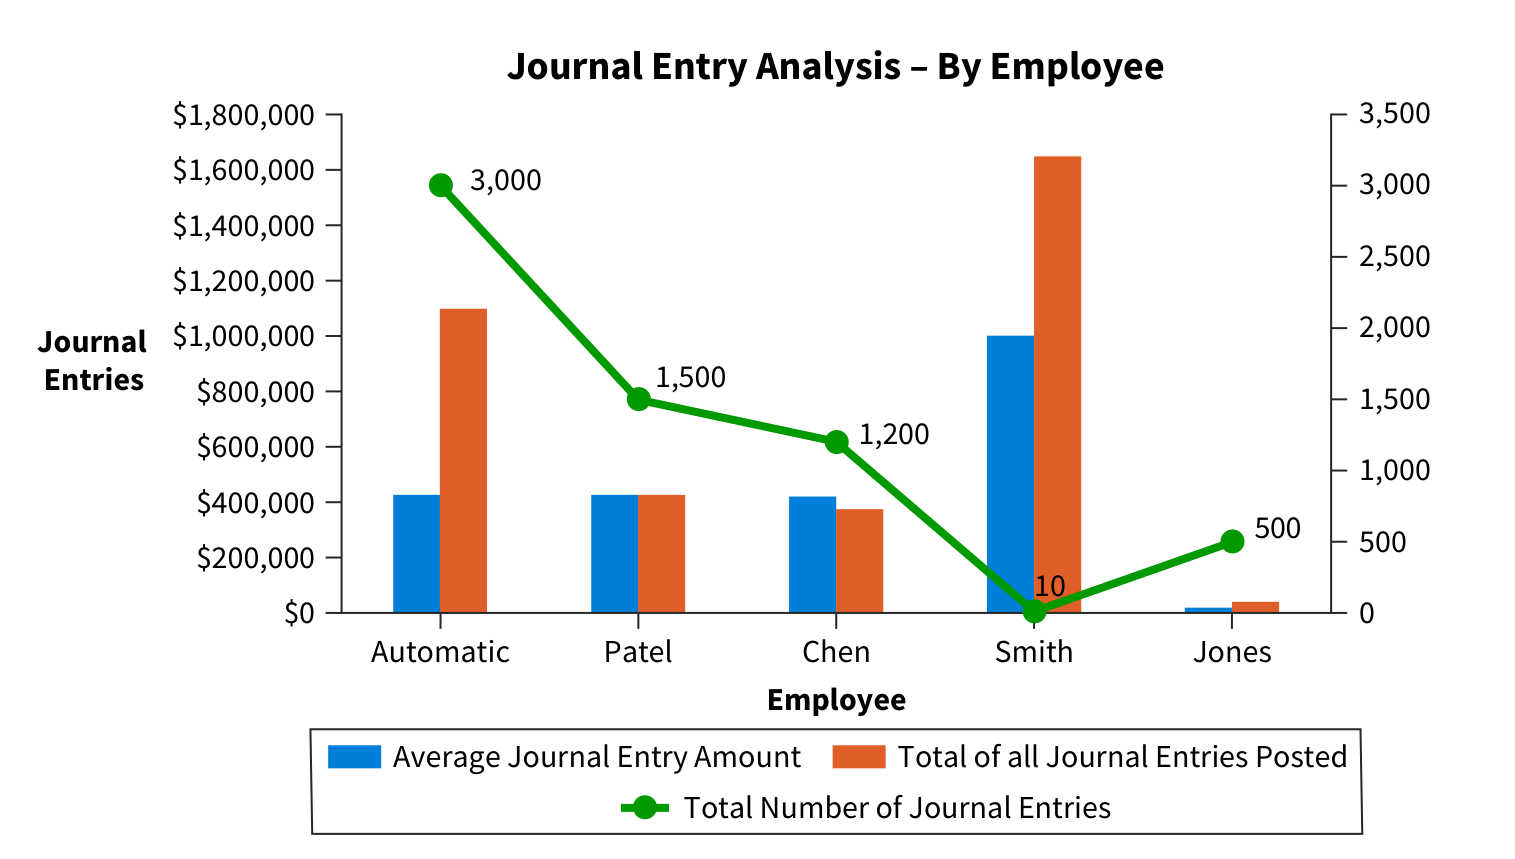
\includegraphics[width=\textwidth,height=0.7\textheight,keepaspectratio]{../textbookForPractice/Figures/Ch_08/EX 8.7.png}
            \end{figure}
        \end{column}
    \end{columns}
\end{frame}

\begin{frame}{EX 8.8 \& EX 8.9}
    \begin{columns}
        \begin{column}{0.5\textwidth}
            \begin{figure}[h]
                \centering
                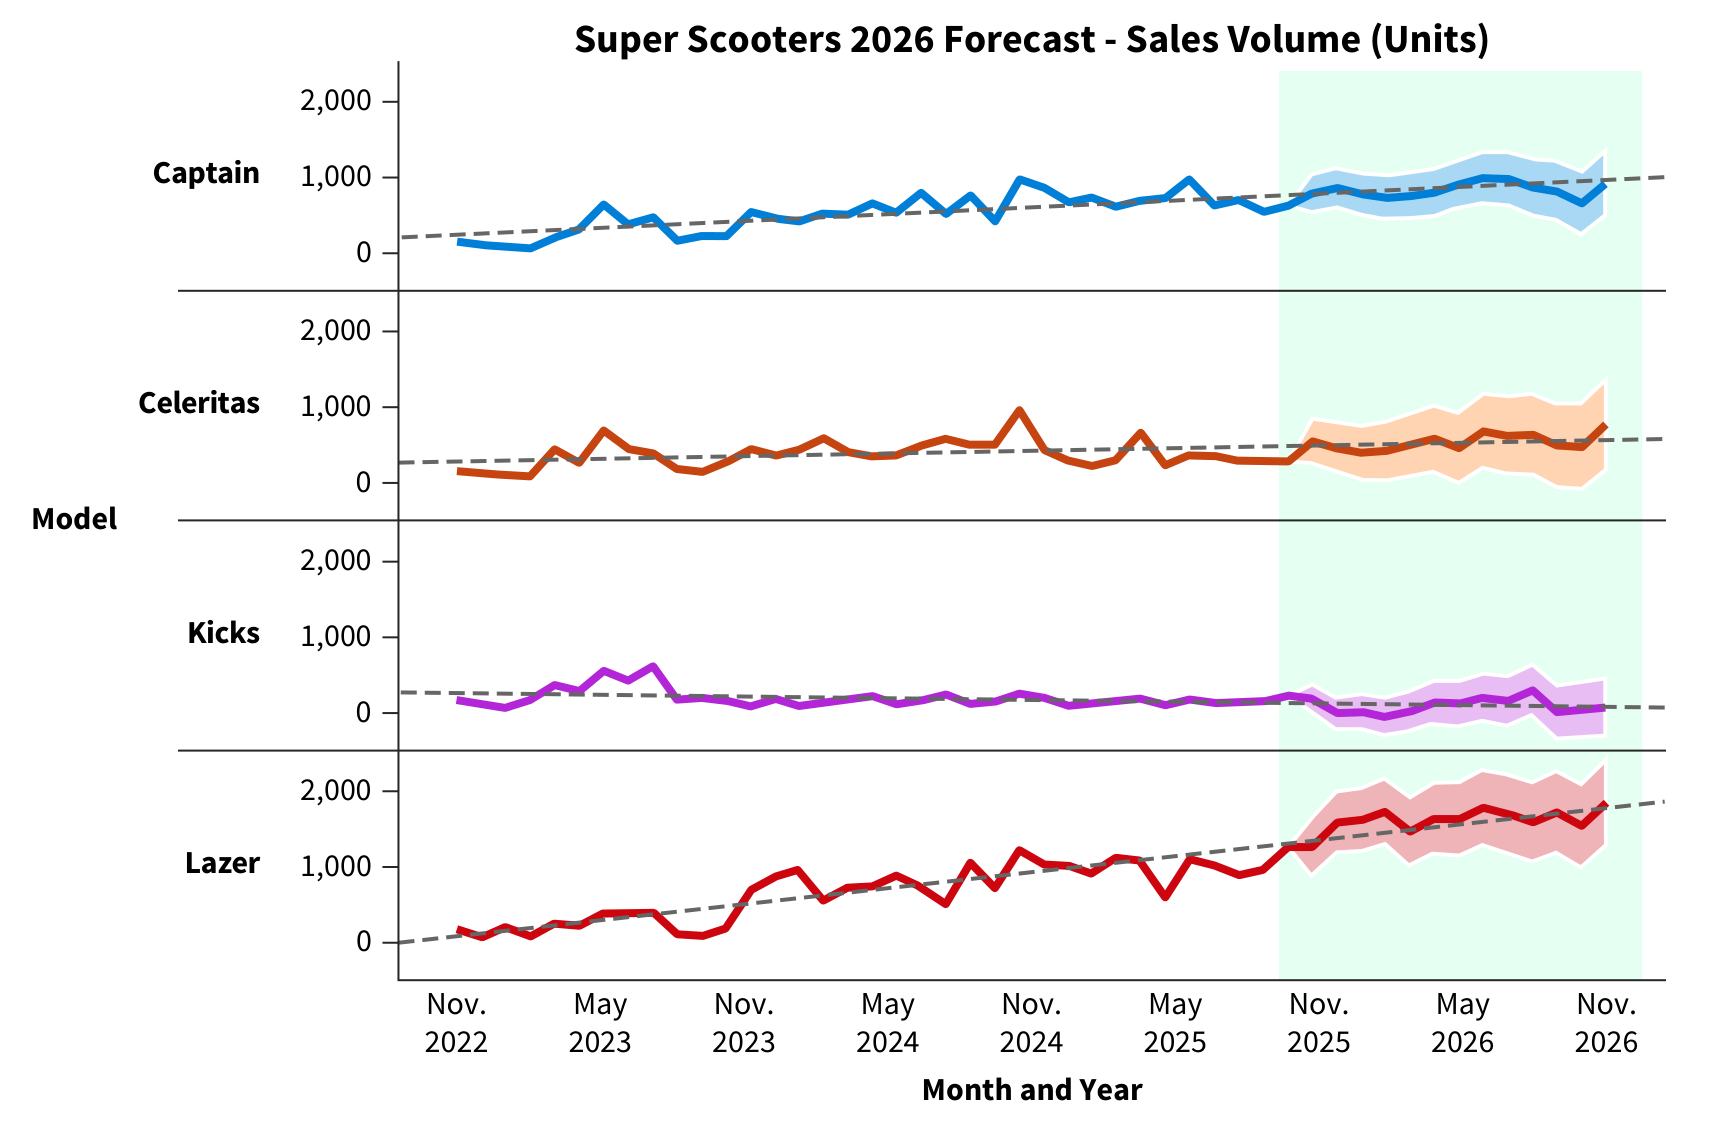
\includegraphics[width=\textwidth,height=0.7\textheight,keepaspectratio]{../textbookForPractice/Figures/Ch_08/EX 8.8.png}
            \end{figure}
        \end{column}
        \begin{column}{0.5\textwidth}
            \begin{figure}[h]
                \centering
                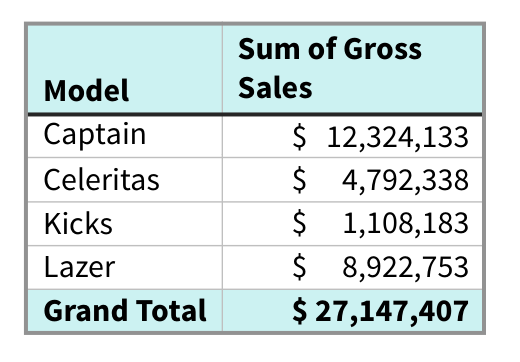
\includegraphics[width=\textwidth,height=0.7\textheight,keepaspectratio]{../textbookForPractice/Figures/Ch_08/EX 8.9.png}
            \end{figure}
        \end{column}
    \end{columns}
\end{frame}

\begin{frame}{EX 8.10 \& EX 8.11}
    \begin{columns}
        \begin{column}{0.5\textwidth}
            \begin{figure}[h]
                \centering
                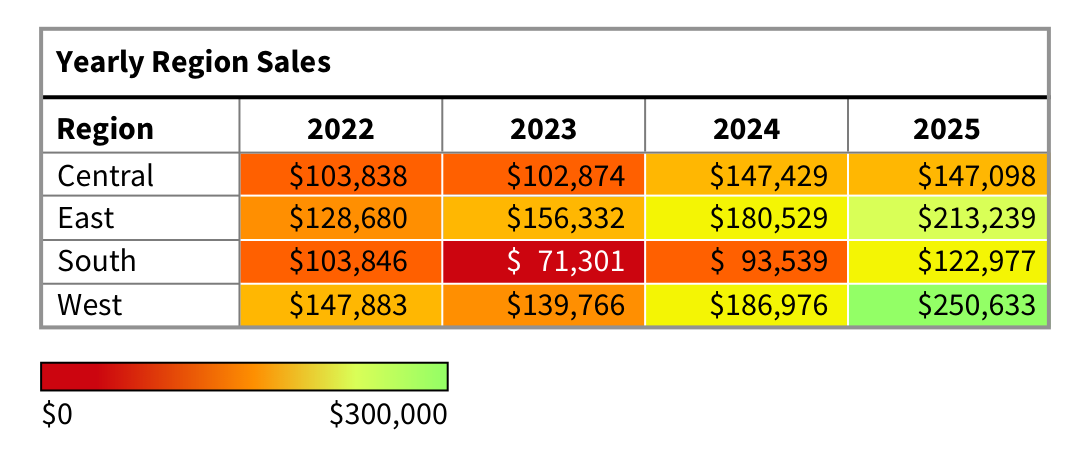
\includegraphics[width=\textwidth,height=0.7\textheight,keepaspectratio]{../textbookForPractice/Figures/Ch_08/EX 8.10.png}
            \end{figure}
        \end{column}
        \begin{column}{0.5\textwidth}
            \begin{figure}[h]
                \centering
                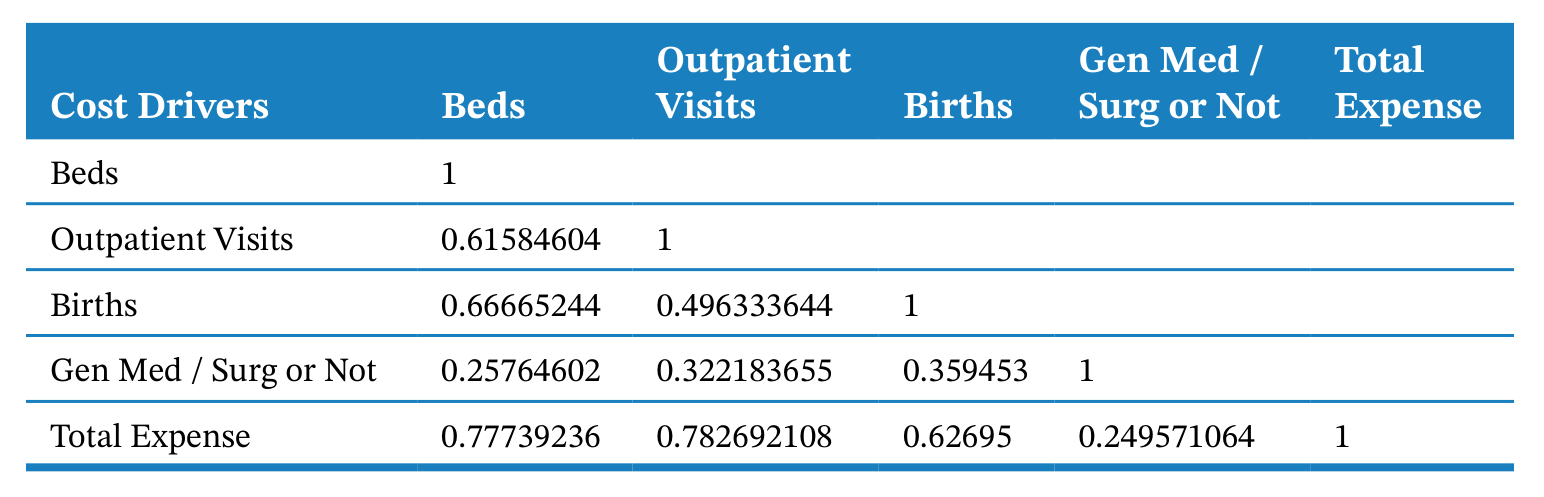
\includegraphics[width=\textwidth,height=0.7\textheight,keepaspectratio]{../textbookForPractice/Figures/Ch_08/EX 8.11.png}
            \end{figure}
        \end{column}
    \end{columns}
\end{frame}

\begin{frame}{EX 8.12 \& EX 8.13}
    \begin{columns}
        \begin{column}{0.5\textwidth}
            \begin{figure}[h]
                \centering
                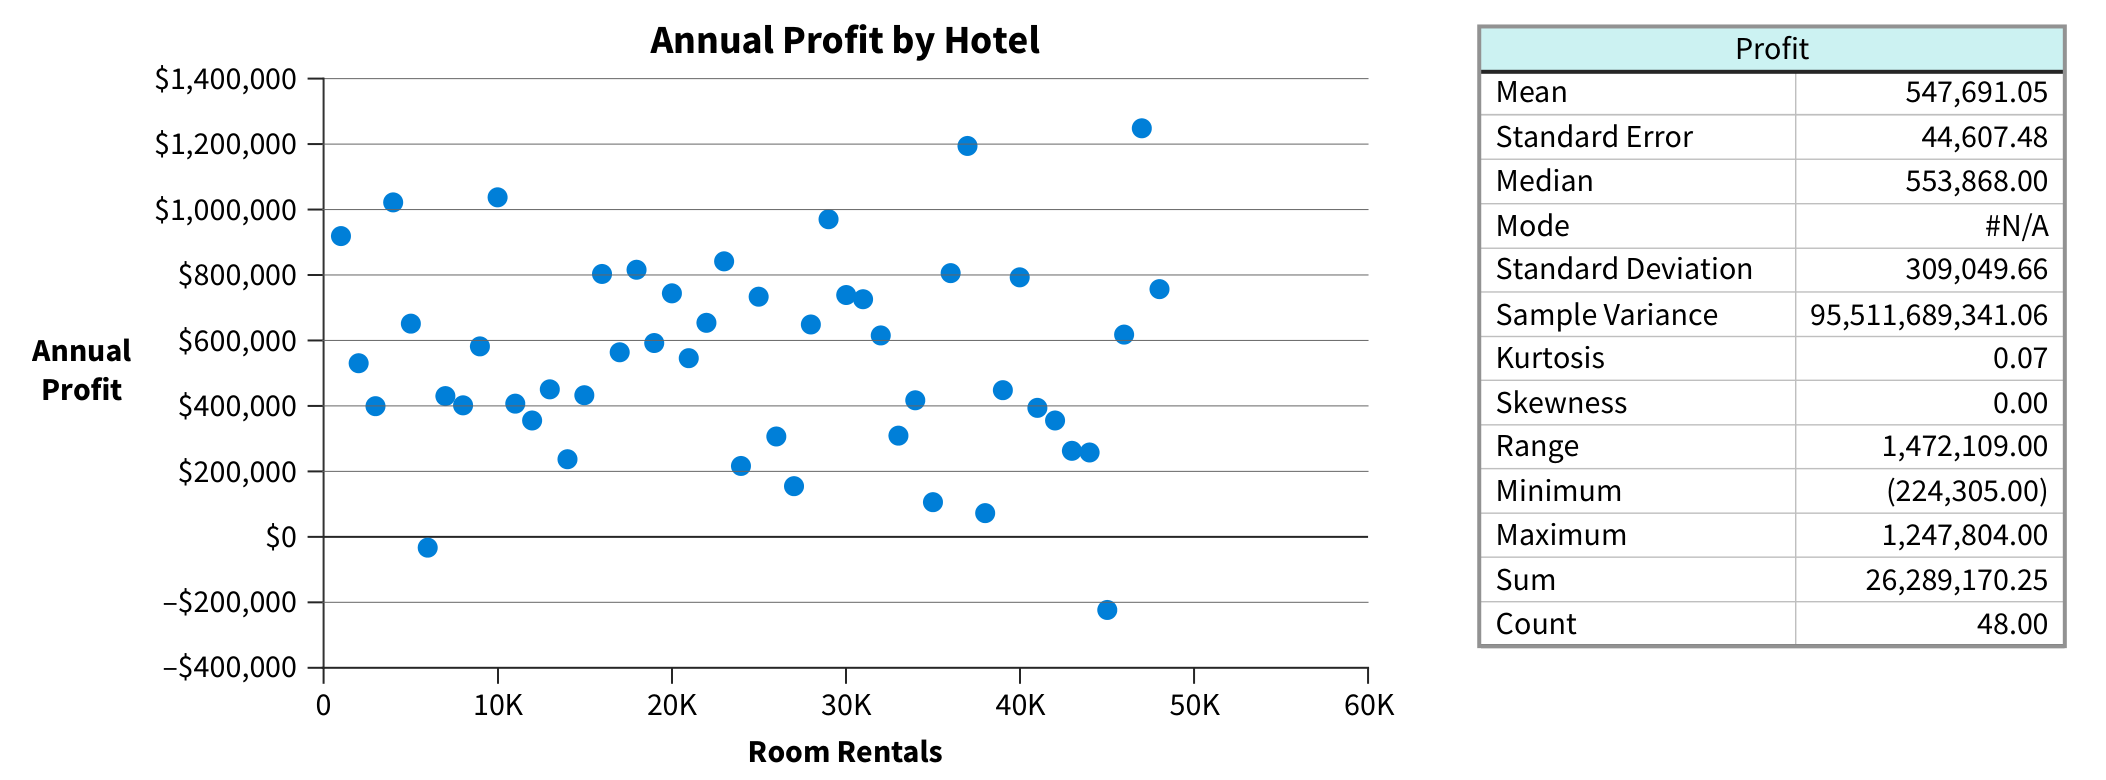
\includegraphics[width=\textwidth,height=0.7\textheight,keepaspectratio]{../textbookForPractice/Figures/Ch_08/EX 8.12.png}
            \end{figure}
        \end{column}
        \begin{column}{0.5\textwidth}
            \begin{figure}[h]
                \centering
                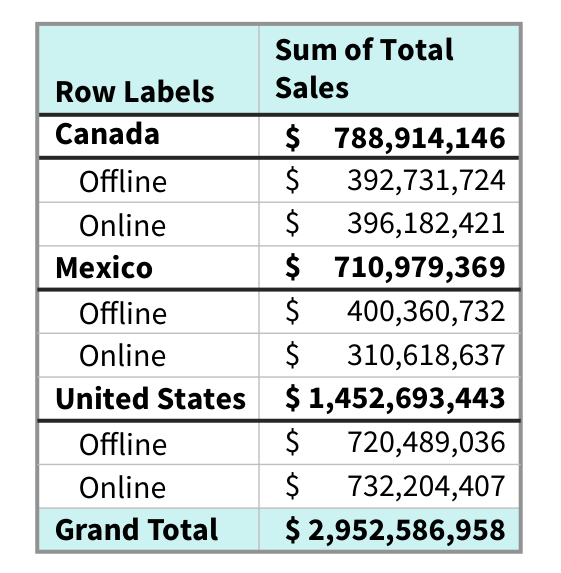
\includegraphics[width=\textwidth,height=0.7\textheight,keepaspectratio]{../textbookForPractice/Figures/Ch_08/EX 8.13.png}
            \end{figure}
        \end{column}
    \end{columns}
\end{frame}

\begin{frame}{EX 8.14 \& EX 8.15}
    \begin{columns}
        \begin{column}{0.5\textwidth}
            \begin{figure}[h]
                \centering
                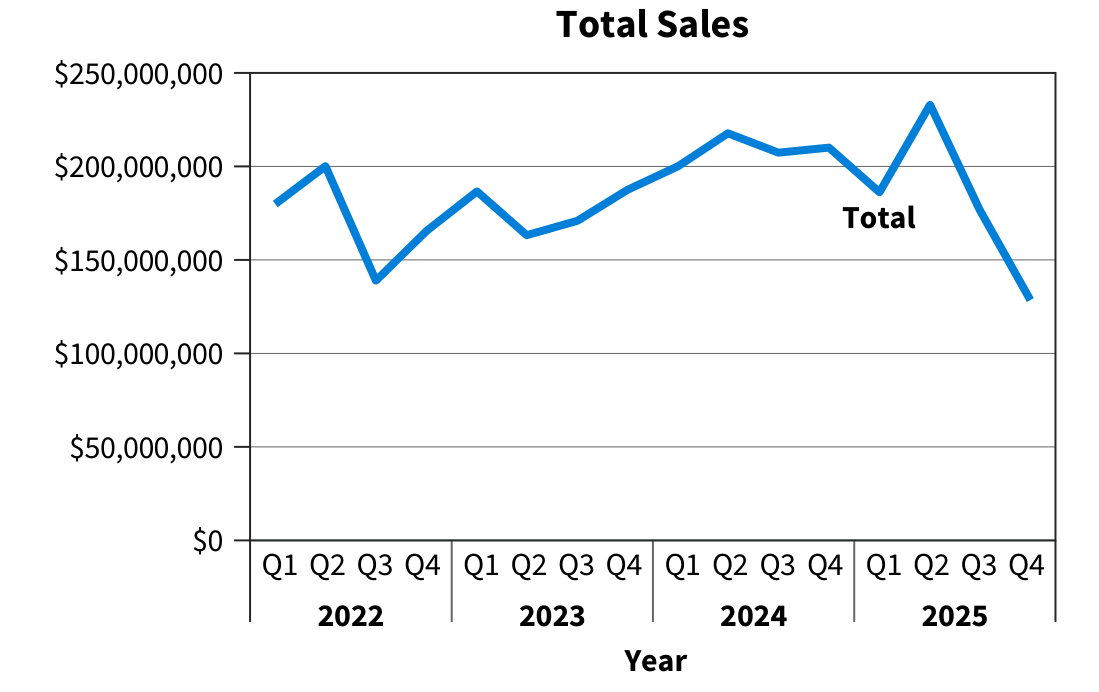
\includegraphics[width=\textwidth,height=0.7\textheight,keepaspectratio]{../textbookForPractice/Figures/Ch_08/EX 8.14.png}
            \end{figure}
        \end{column}
        \begin{column}{0.5\textwidth}
            \begin{figure}[h]
                \centering
                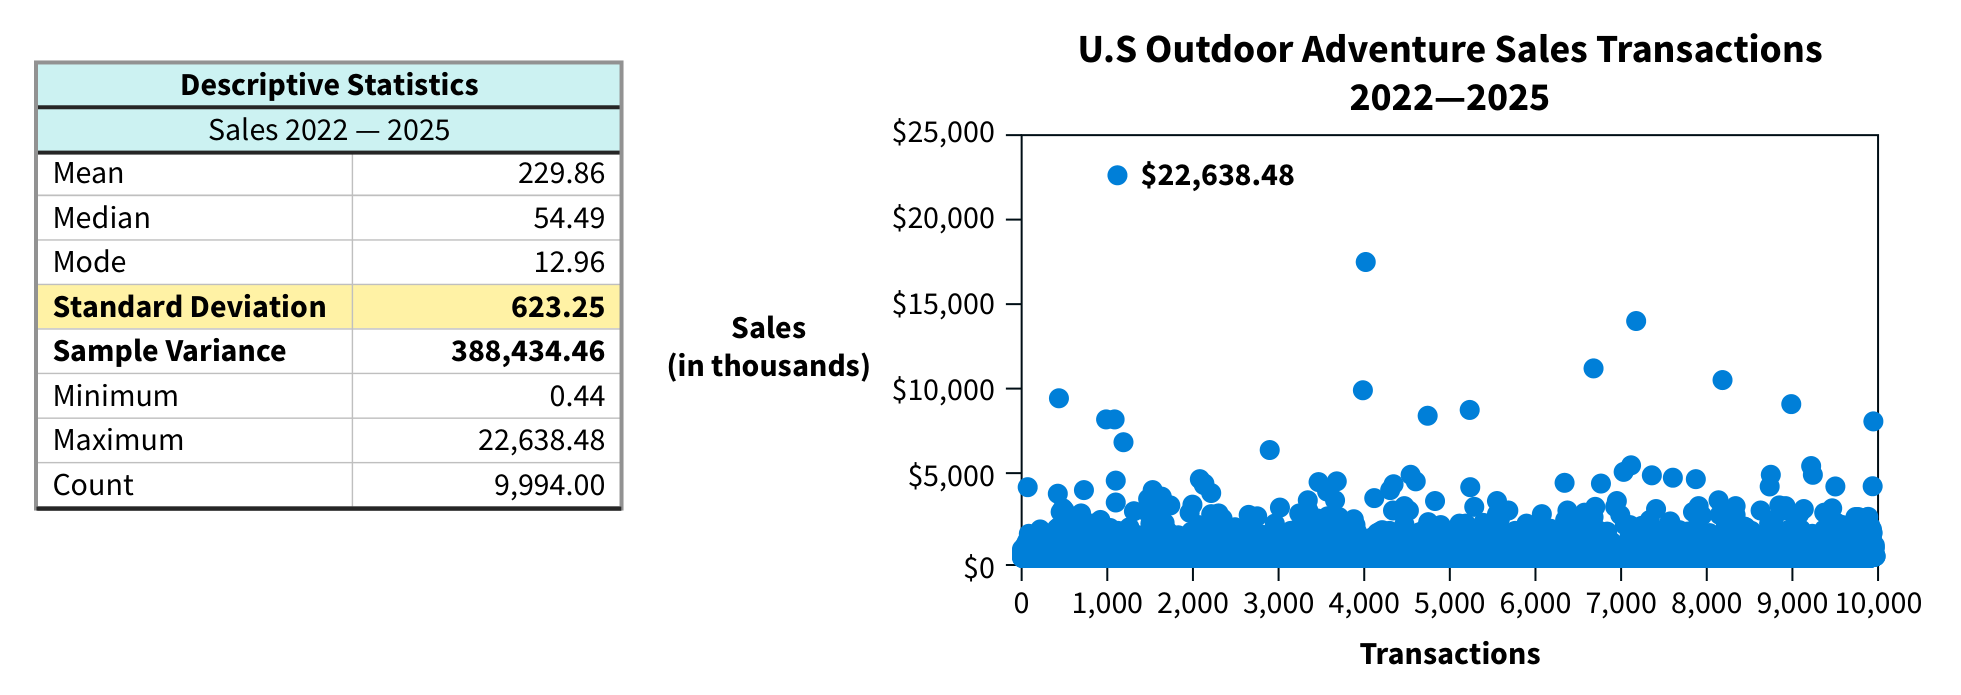
\includegraphics[width=\textwidth,height=0.7\textheight,keepaspectratio]{../textbookForPractice/Figures/Ch_08/EX 8.15.png}
            \end{figure}
        \end{column}
    \end{columns}
\end{frame}

\begin{frame}{EX 8.16 \& EX 8.17A}
    \begin{columns}
        \begin{column}{0.5\textwidth}
            \begin{figure}[h]
                \centering
                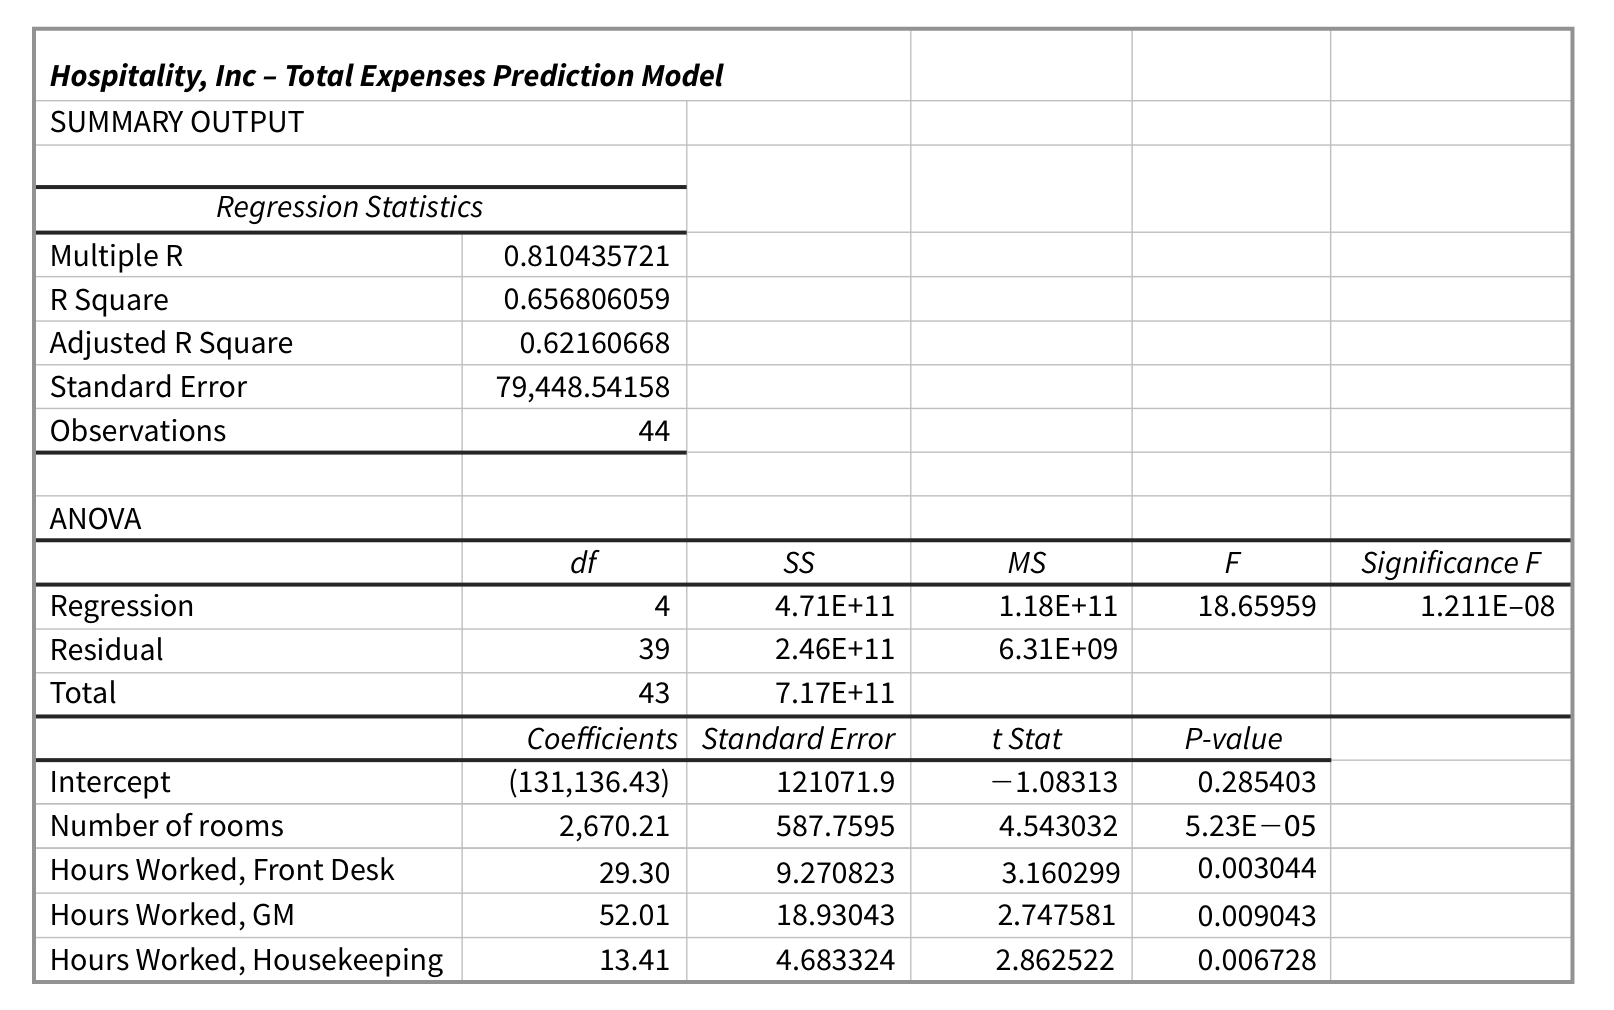
\includegraphics[width=\textwidth,height=0.7\textheight,keepaspectratio]{../textbookForPractice/Figures/Ch_08/EX 8.16.png}
            \end{figure}
        \end{column}
        \begin{column}{0.5\textwidth}
            \begin{figure}[h]
                \centering
                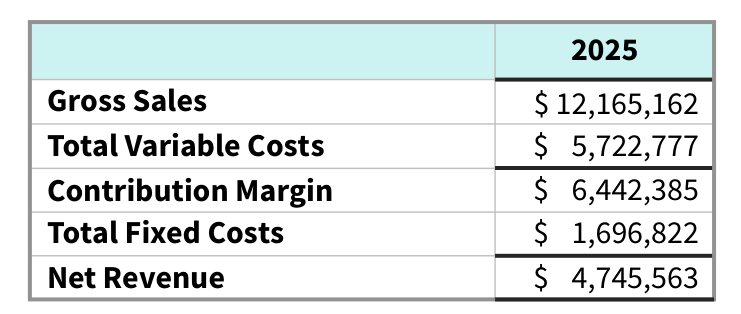
\includegraphics[width=\textwidth,height=0.7\textheight,keepaspectratio]{../textbookForPractice/Figures/Ch_08/EX 8.17A.png}
            \end{figure}
        \end{column}
    \end{columns}
\end{frame}

\begin{frame}{EX 8.17B \& EX 8.19}
    \begin{columns}
        \begin{column}{0.5\textwidth}
            \begin{figure}[h]
                \centering
                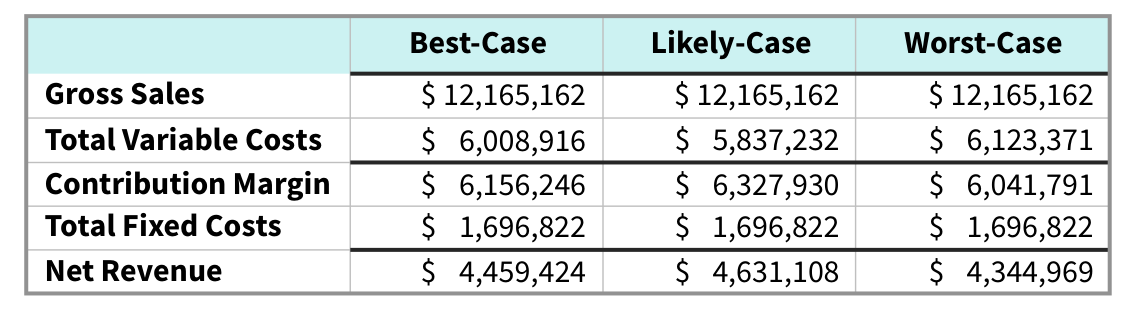
\includegraphics[width=\textwidth,height=0.7\textheight,keepaspectratio]{../textbookForPractice/Figures/Ch_08/EX 8.17B.png}
            \end{figure}
        \end{column}
        \begin{column}{0.5\textwidth}
            \begin{figure}[h]
                \centering
                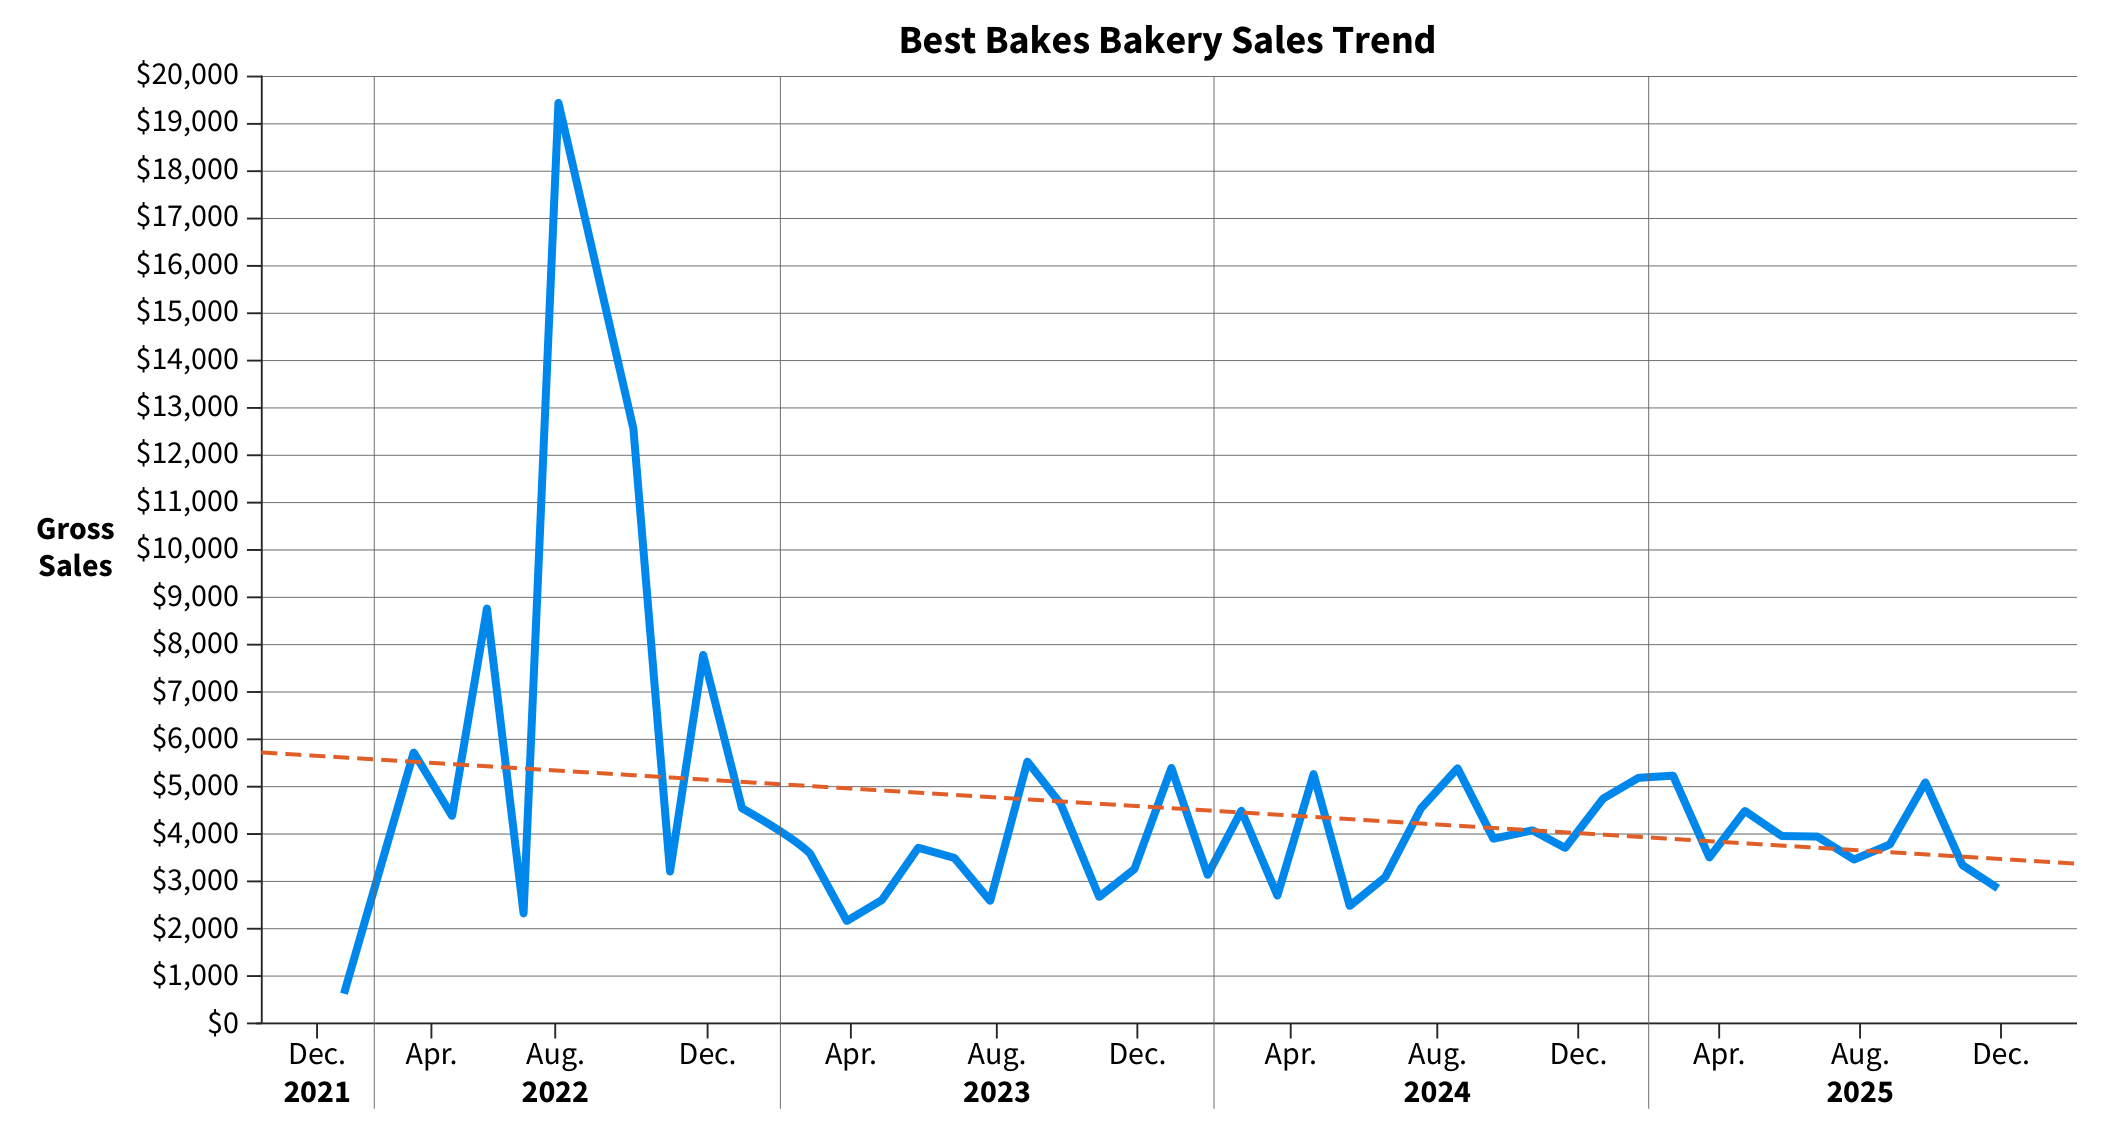
\includegraphics[width=\textwidth,height=0.7\textheight,keepaspectratio]{../textbookForPractice/Figures/Ch_08/EX 8.19.png}
            \end{figure}
        \end{column}
    \end{columns}
\end{frame}

\begin{frame}{EX 8.20}

    \begin{figure}[h]
        \centering
        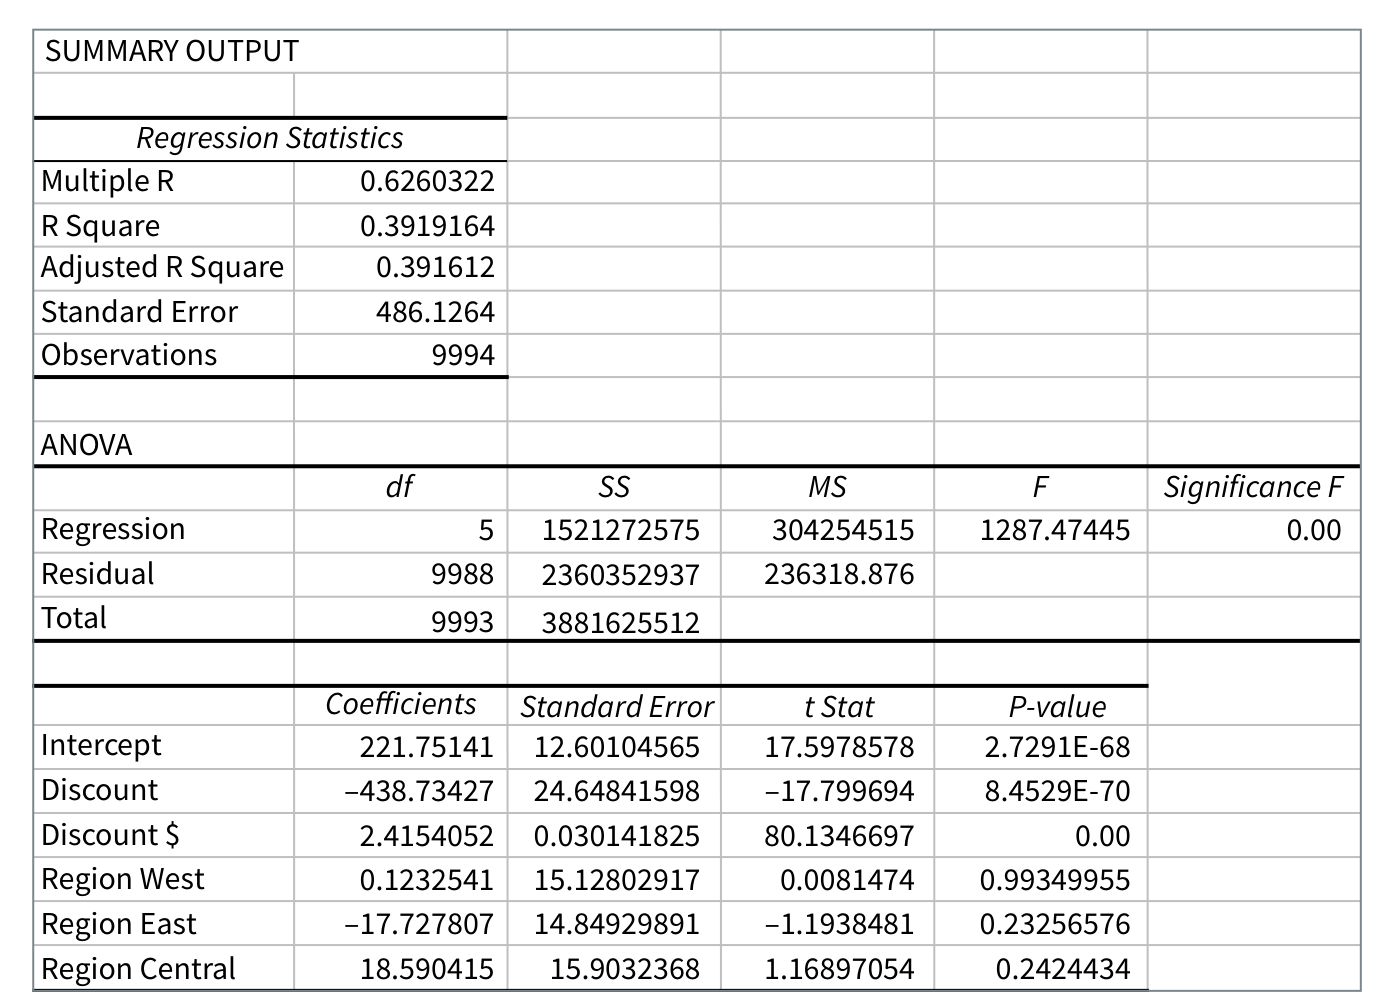
\includegraphics[width=0.95\textwidth,height=0.75\textheight,keepaspectratio]{../textbookForPractice/Figures/Ch_08/EX 8.20.png}
    \end{figure}
\end{frame}

\begin{frame}{Tình huống Ứng dụng (PAC)}
\begin{center}
        \Huge \textbf{Tình huống Ứng dụng Chuyên môn} \\
        \vspace{0.5cm}
        \Large Professional Application Cases (PAC)
    \end{center}
\end{frame}

\begin{frame}{PAC 8.1A \& PAC 8.1b}
    \begin{columns}
        \begin{column}{0.5\textwidth}
            \begin{figure}[h]
                \centering
                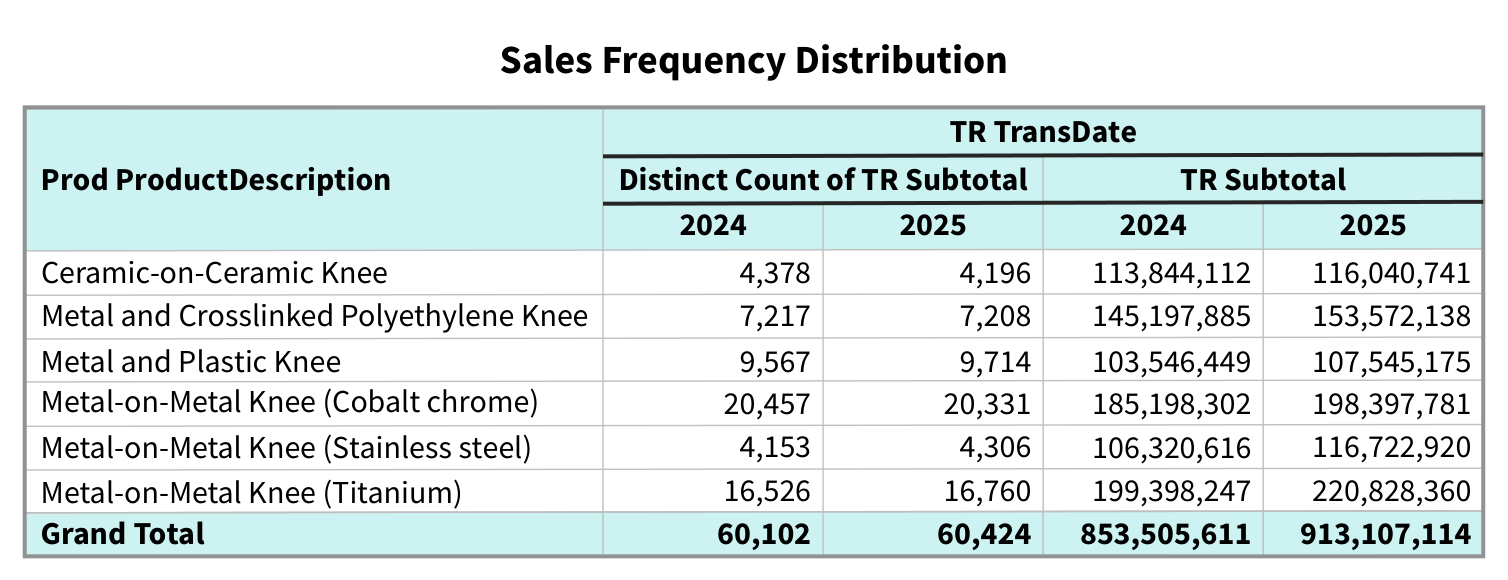
\includegraphics[width=\textwidth,height=0.7\textheight,keepaspectratio]{../textbookForPractice/Figures/Ch_08/PAC 8.1A.png}
            \end{figure}
        \end{column}
        \begin{column}{0.5\textwidth}
            \begin{figure}[h]
                \centering
                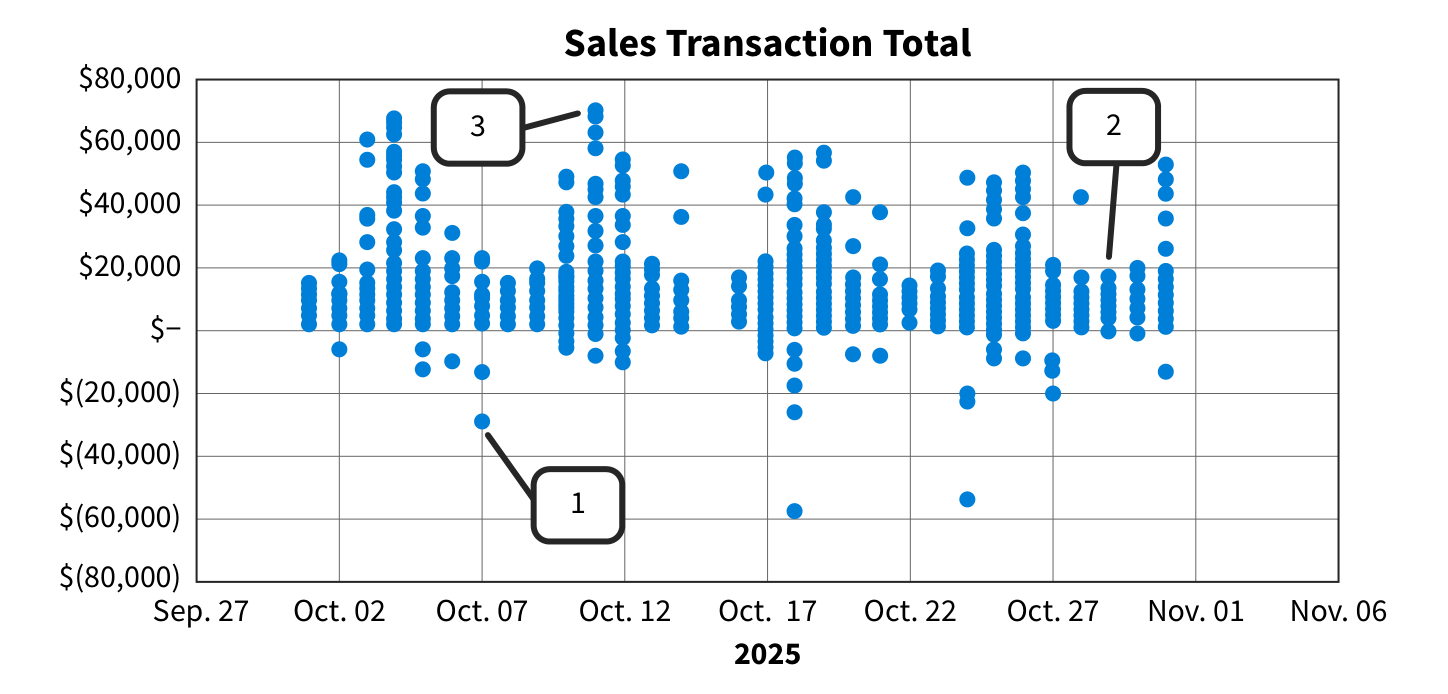
\includegraphics[width=\textwidth,height=0.7\textheight,keepaspectratio]{../textbookForPractice/Figures/Ch_08/PAC 8.1b.png}
            \end{figure}
        \end{column}
    \end{columns}
\end{frame}

\begin{frame}{PAC 8.1A\_1 \& PAC 8.2}
    \begin{columns}
        \begin{column}{0.5\textwidth}
            \begin{figure}[h]
                \centering
                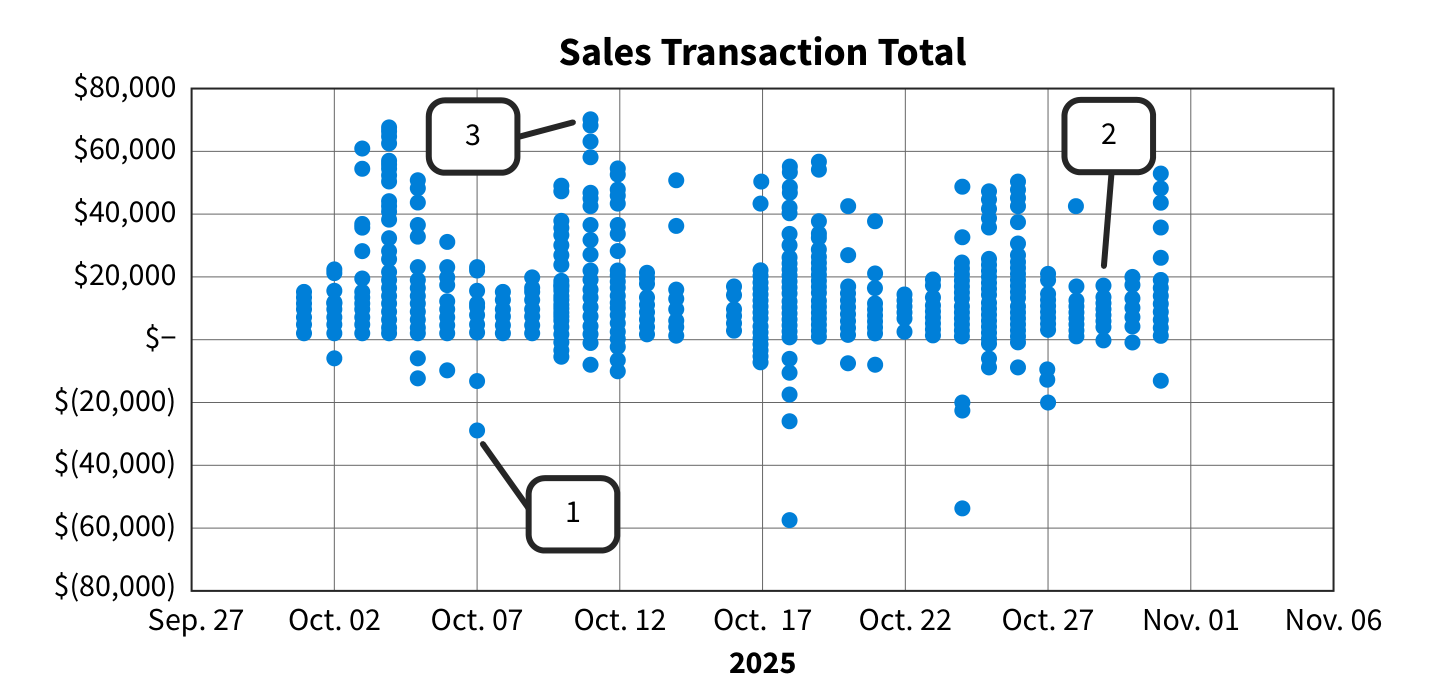
\includegraphics[width=\textwidth,height=0.7\textheight,keepaspectratio]{../textbookForPractice/Figures/Ch_08/PAC 8.1A_1.png}
            \end{figure}
        \end{column}
        \begin{column}{0.5\textwidth}
            \begin{figure}[h]
                \centering
                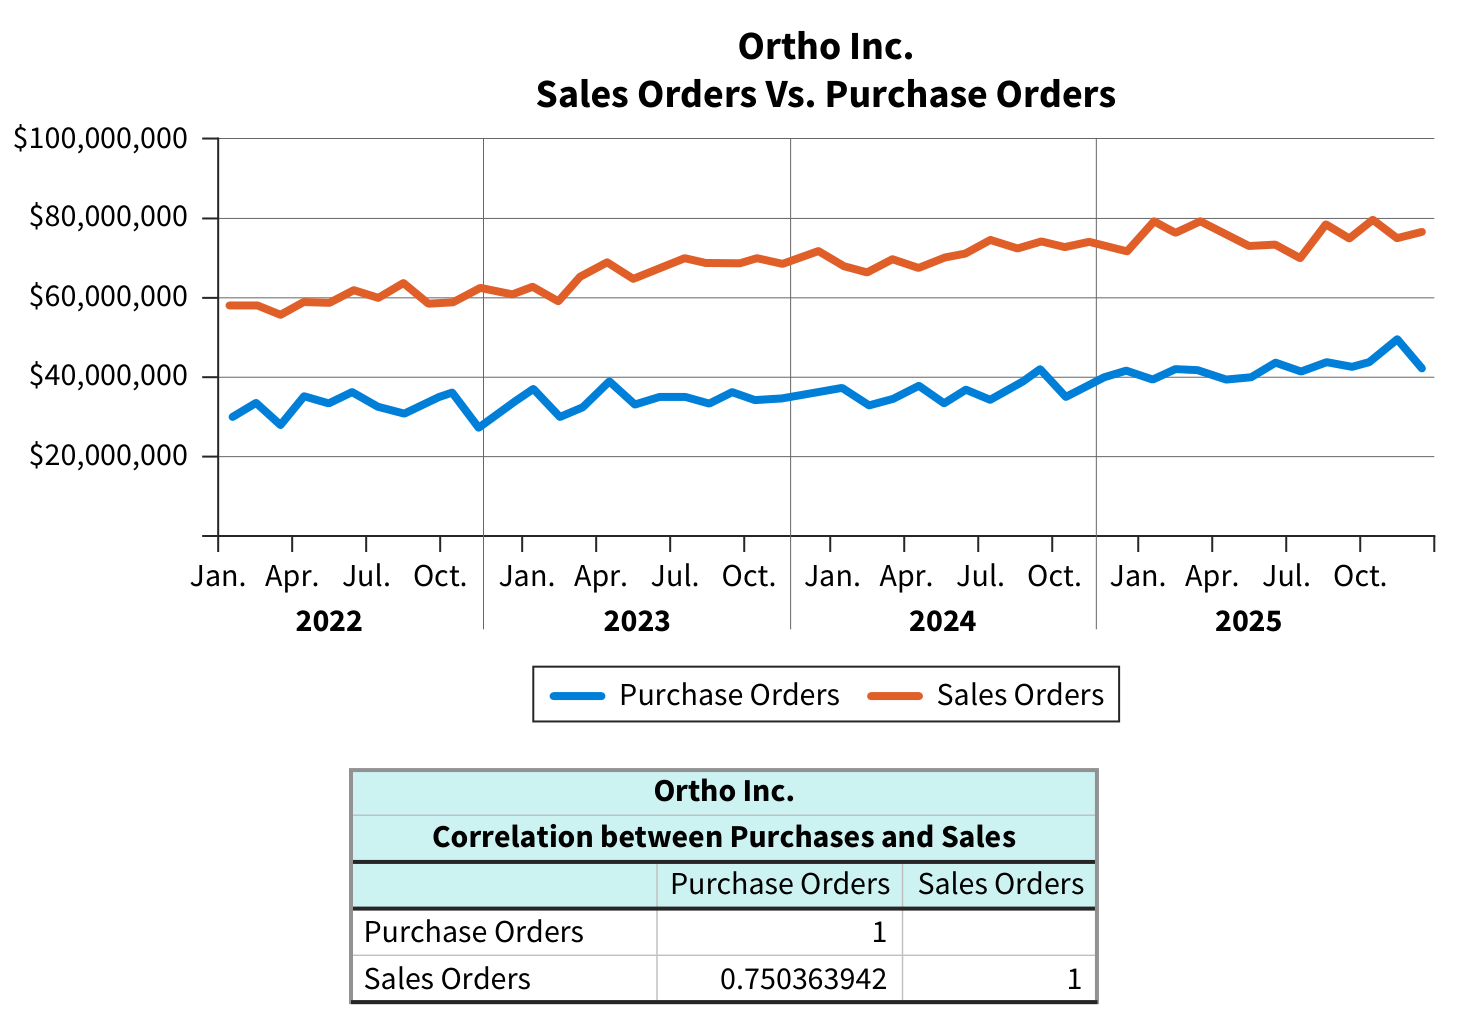
\includegraphics[width=\textwidth,height=0.7\textheight,keepaspectratio]{../textbookForPractice/Figures/Ch_08/PAC 8.2.png}
            \end{figure}
        \end{column}
    \end{columns}
\end{frame}

\begin{frame}{PAC 8.3 \& PAC 8.4}
    \begin{columns}
        \begin{column}{0.5\textwidth}
            \begin{figure}[h]
                \centering
                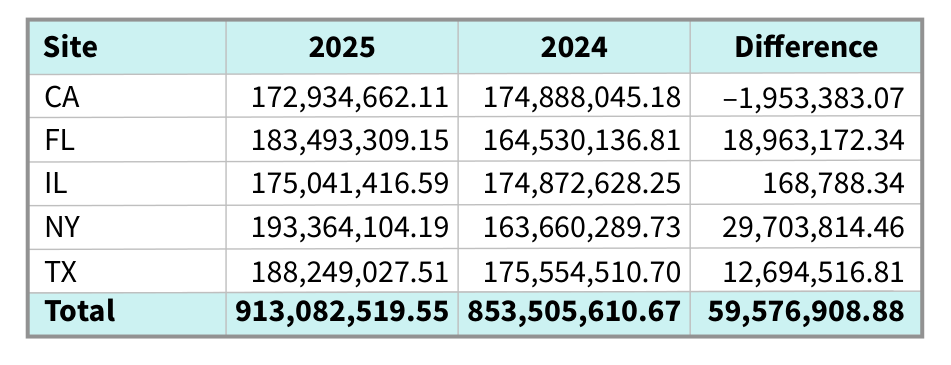
\includegraphics[width=\textwidth,height=0.7\textheight,keepaspectratio]{../textbookForPractice/Figures/Ch_08/PAC 8.3.png}
            \end{figure}
        \end{column}
        \begin{column}{0.5\textwidth}
            \begin{figure}[h]
                \centering
                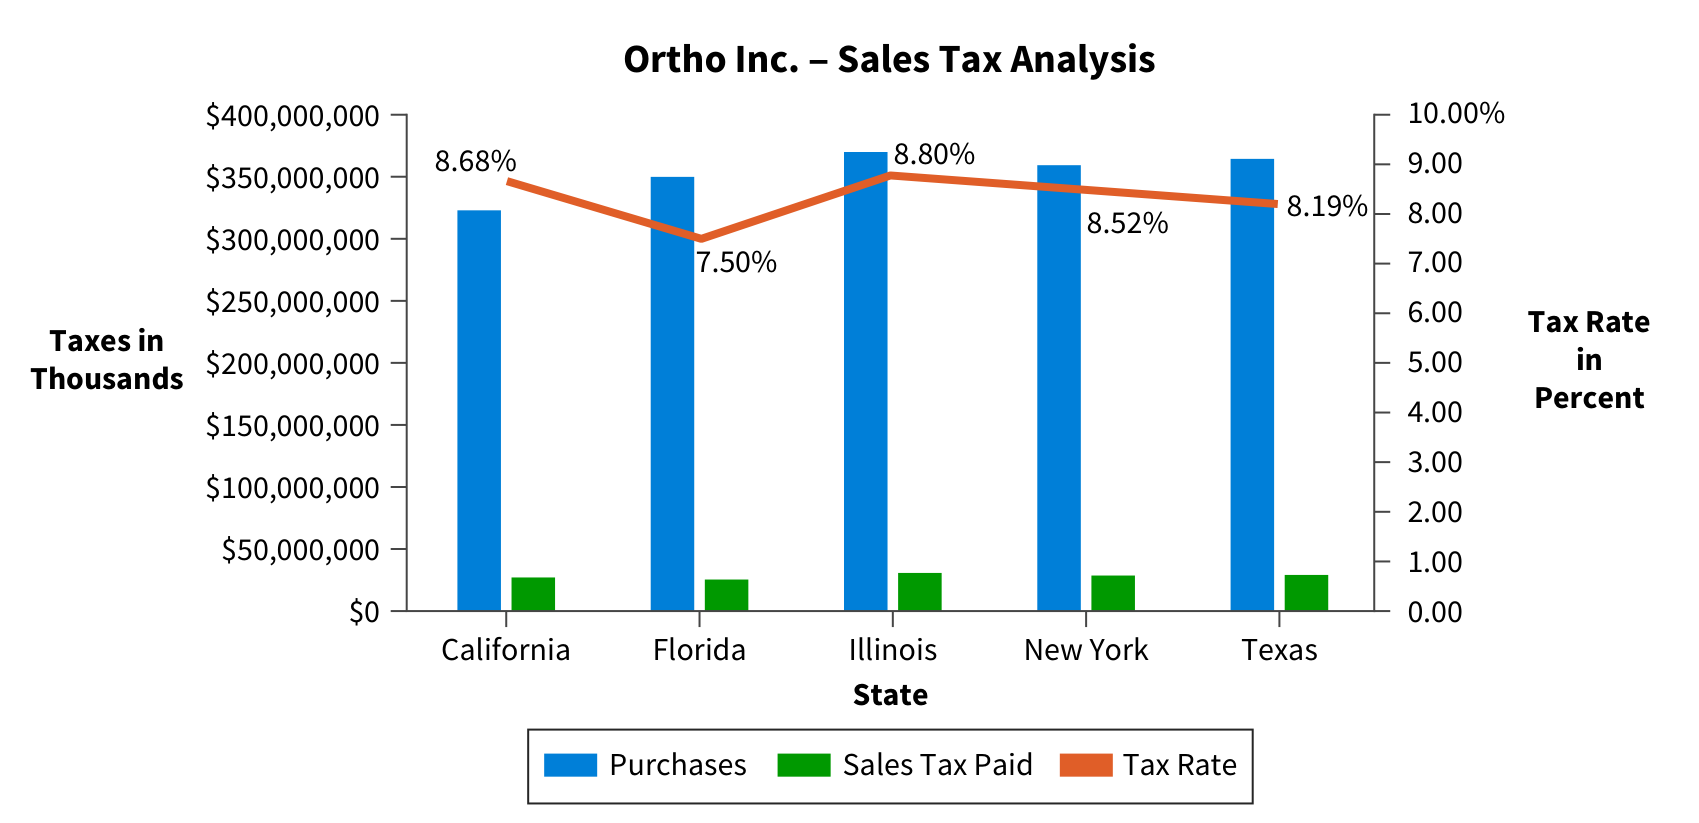
\includegraphics[width=\textwidth,height=0.7\textheight,keepaspectratio]{../textbookForPractice/Figures/Ch_08/PAC 8.4.png}
            \end{figure}
        \end{column}
    \end{columns}
\end{frame}

\begin{frame}{Trường hợp và Bổ trợ}
\begin{center}
        \Huge \textbf{Tình huống Bổ trợ \& Dữ liệu} \\
        \vspace{0.5cm}
        \Large PR, ERD, Info
    \end{center}
\end{frame}

\begin{frame}{LO 2.4}

    \begin{figure}[h]
        \centering
        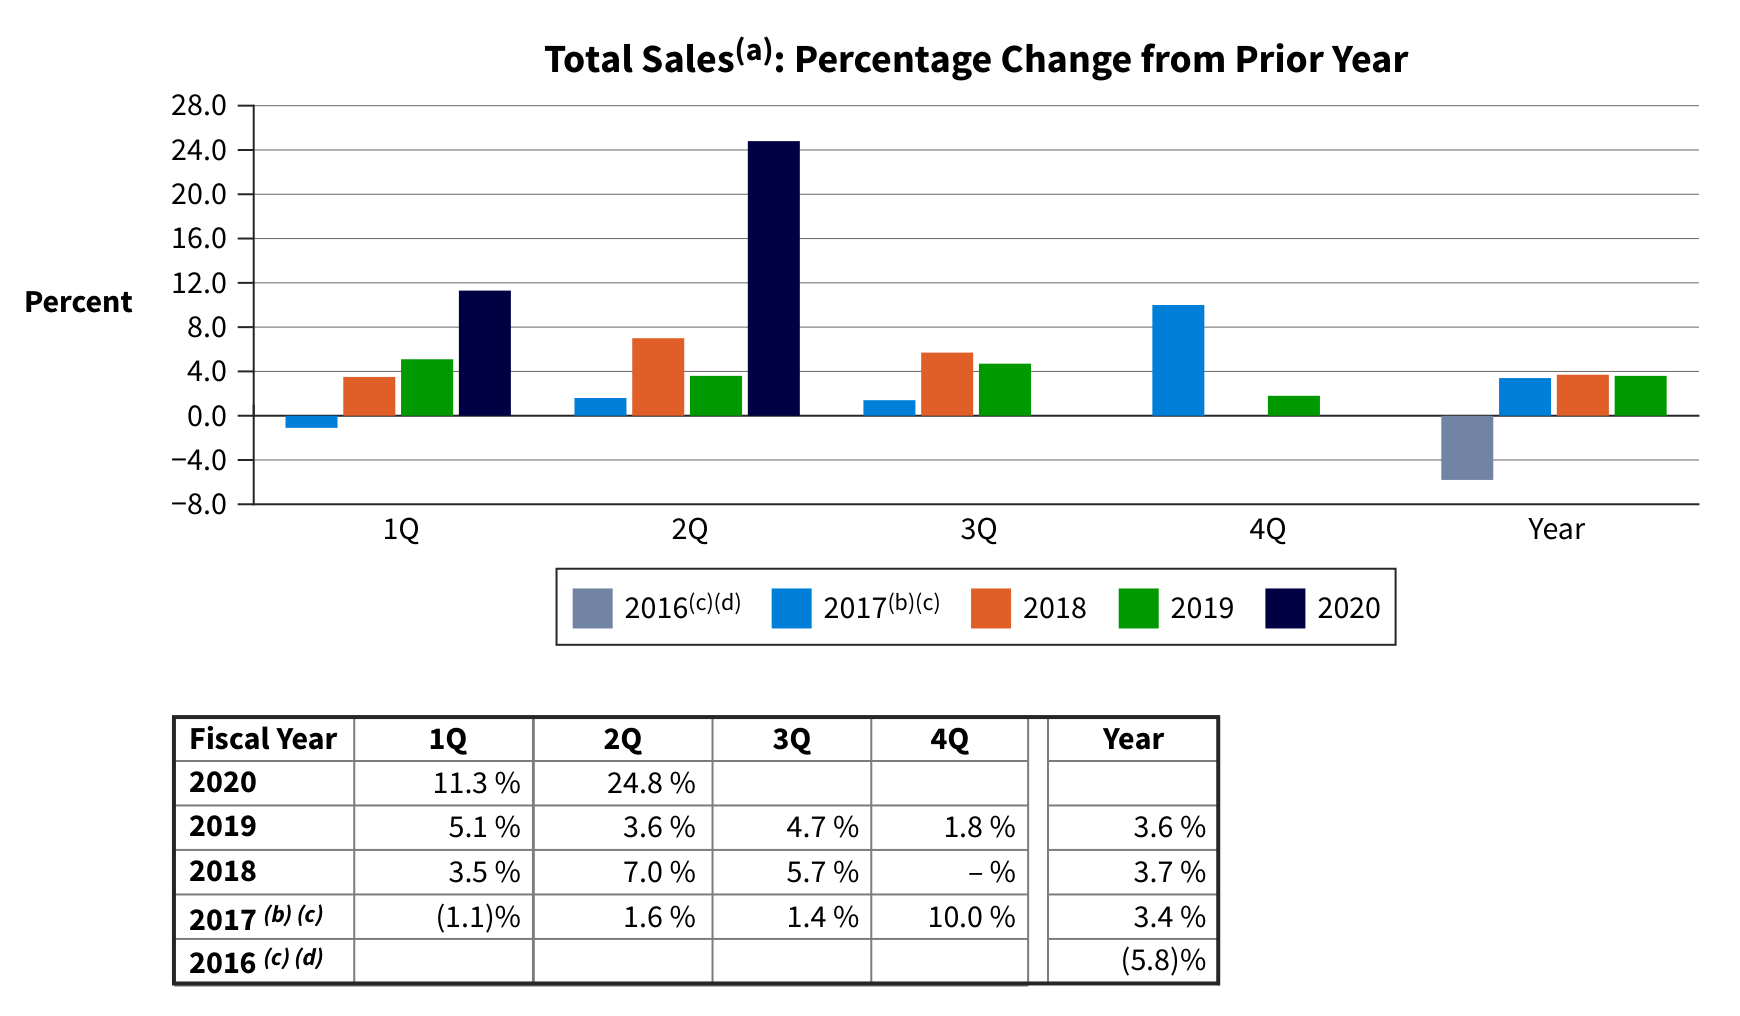
\includegraphics[width=0.95\textwidth,height=0.75\textheight,keepaspectratio]{../textbookForPractice/Figures/Ch_08/LO 2.4.png}
    \end{figure}
\end{frame}

\begin{frame}{Infor 8.0}

    \begin{figure}[h]
        \centering
        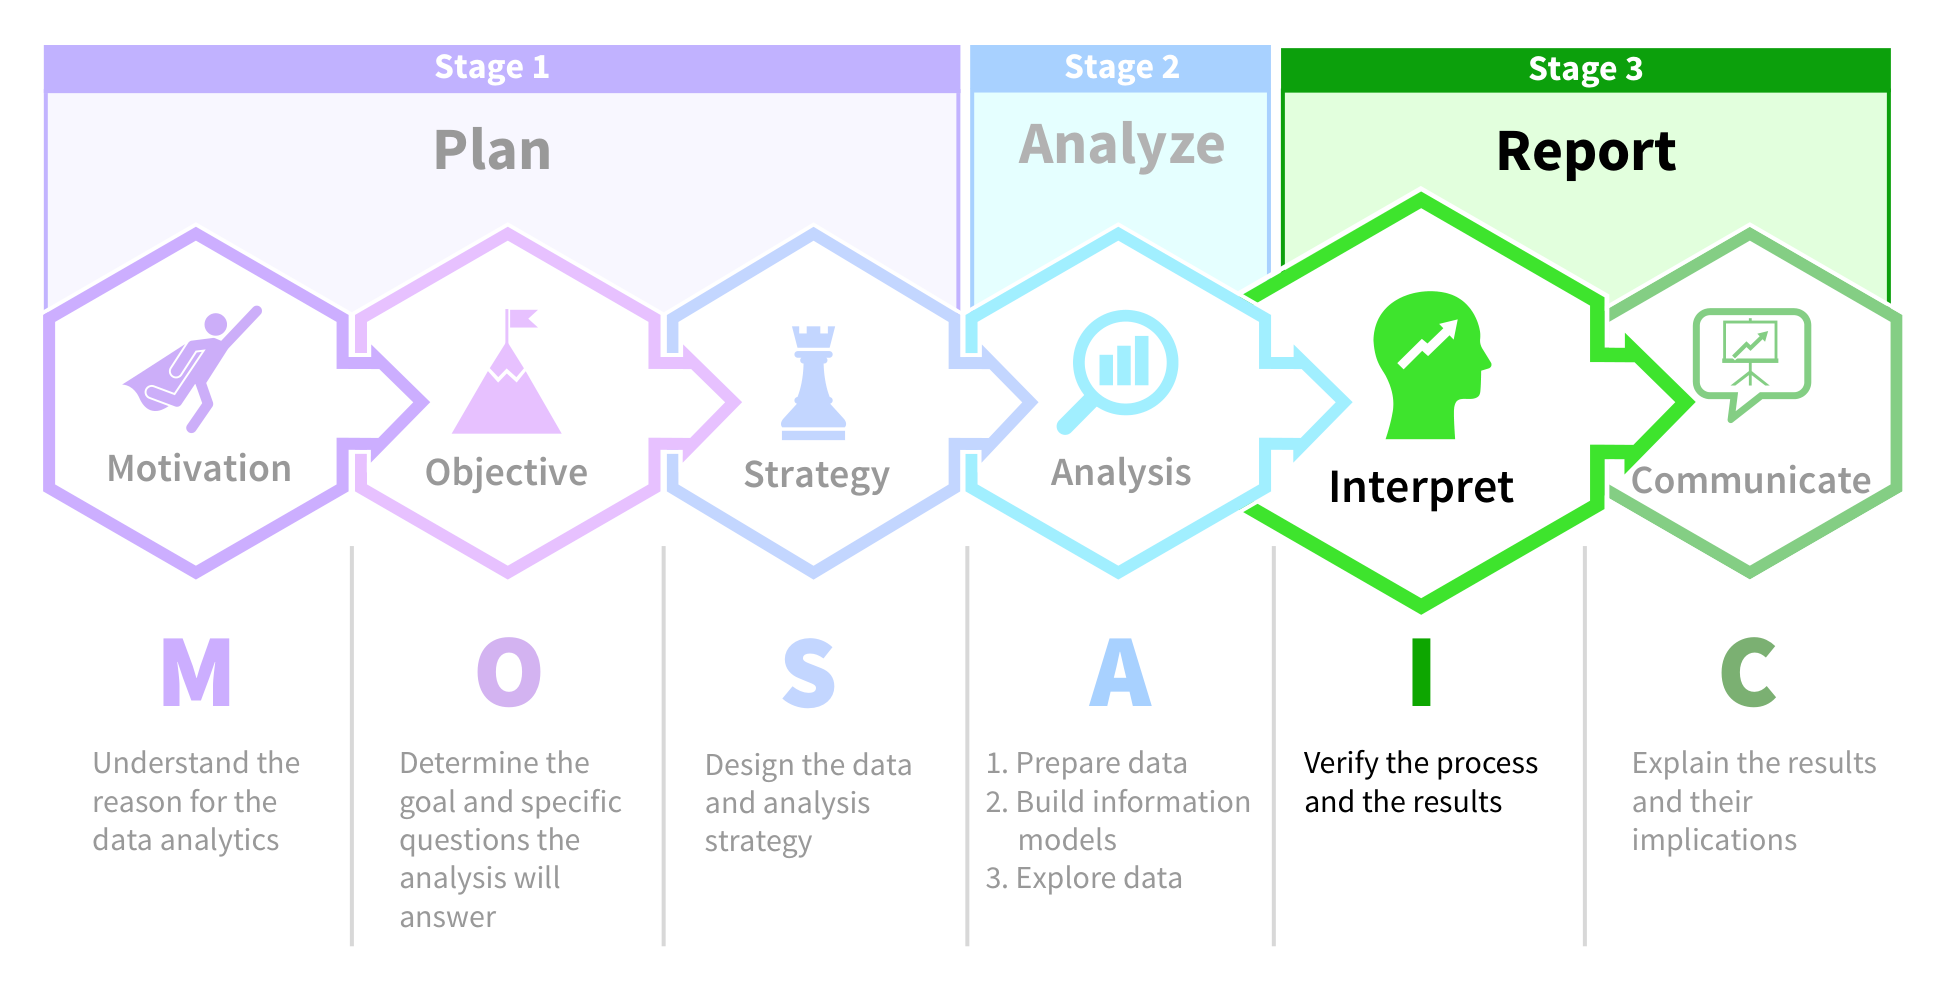
\includegraphics[width=0.95\textwidth,height=0.75\textheight,keepaspectratio]{../textbookForPractice/Figures/Ch_08/Infor 8.0.png}
    \end{figure}
\end{frame}

\begin{frame}{Ortho Inc 8.0}

    \begin{figure}[h]
        \centering
        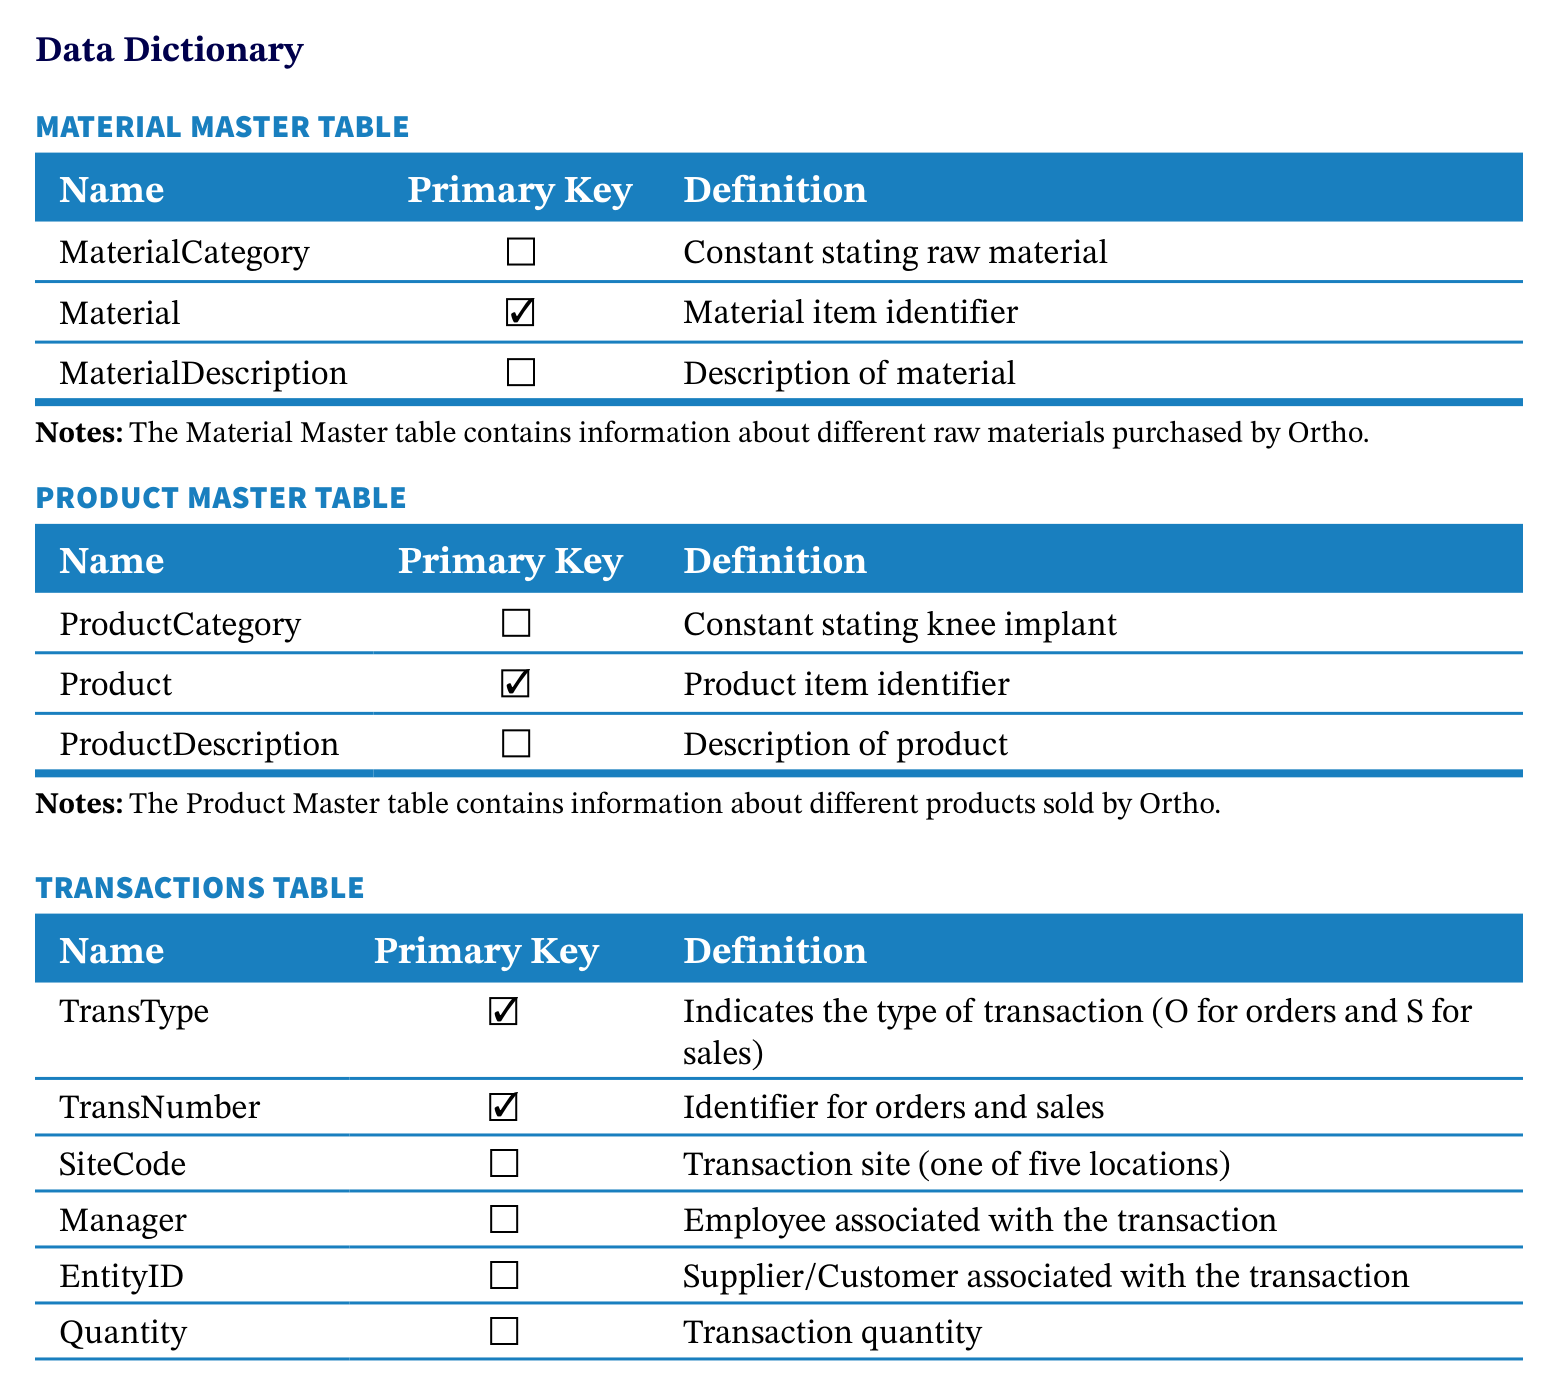
\includegraphics[width=0.95\textwidth,height=0.75\textheight,keepaspectratio]{../textbookForPractice/Figures/Ch_08/Ortho Inc 8.0.png}
    \end{figure}
\end{frame}

\begin{frame}{Apply It 8.1A}

    \begin{figure}[h]
        \centering
        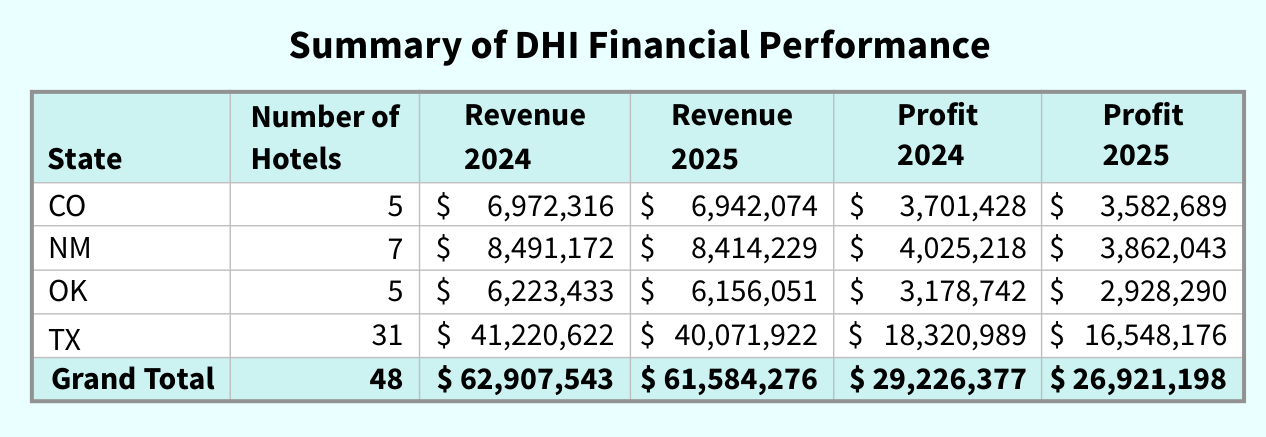
\includegraphics[width=0.95\textwidth,height=0.75\textheight,keepaspectratio]{../textbookForPractice/Figures/Ch_08/Apply It 8.1A.png}
    \end{figure}
\end{frame}

\begin{frame}{Apply It 8.1B}

    \begin{figure}[h]
        \centering
        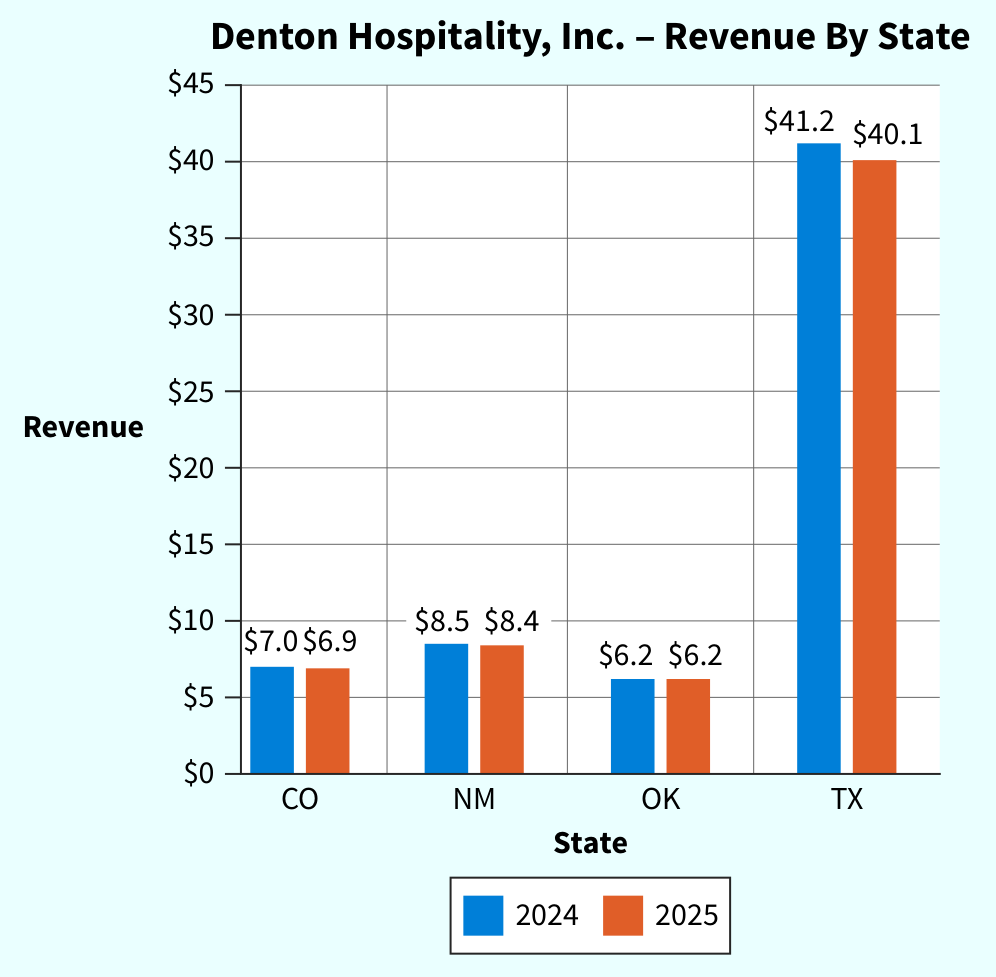
\includegraphics[width=0.95\textwidth,height=0.75\textheight,keepaspectratio]{../textbookForPractice/Figures/Ch_08/Apply It 8.1B.png}
    \end{figure}
\end{frame}

\begin{frame}{ERD 8.1A}

    \begin{figure}[h]
        \centering
        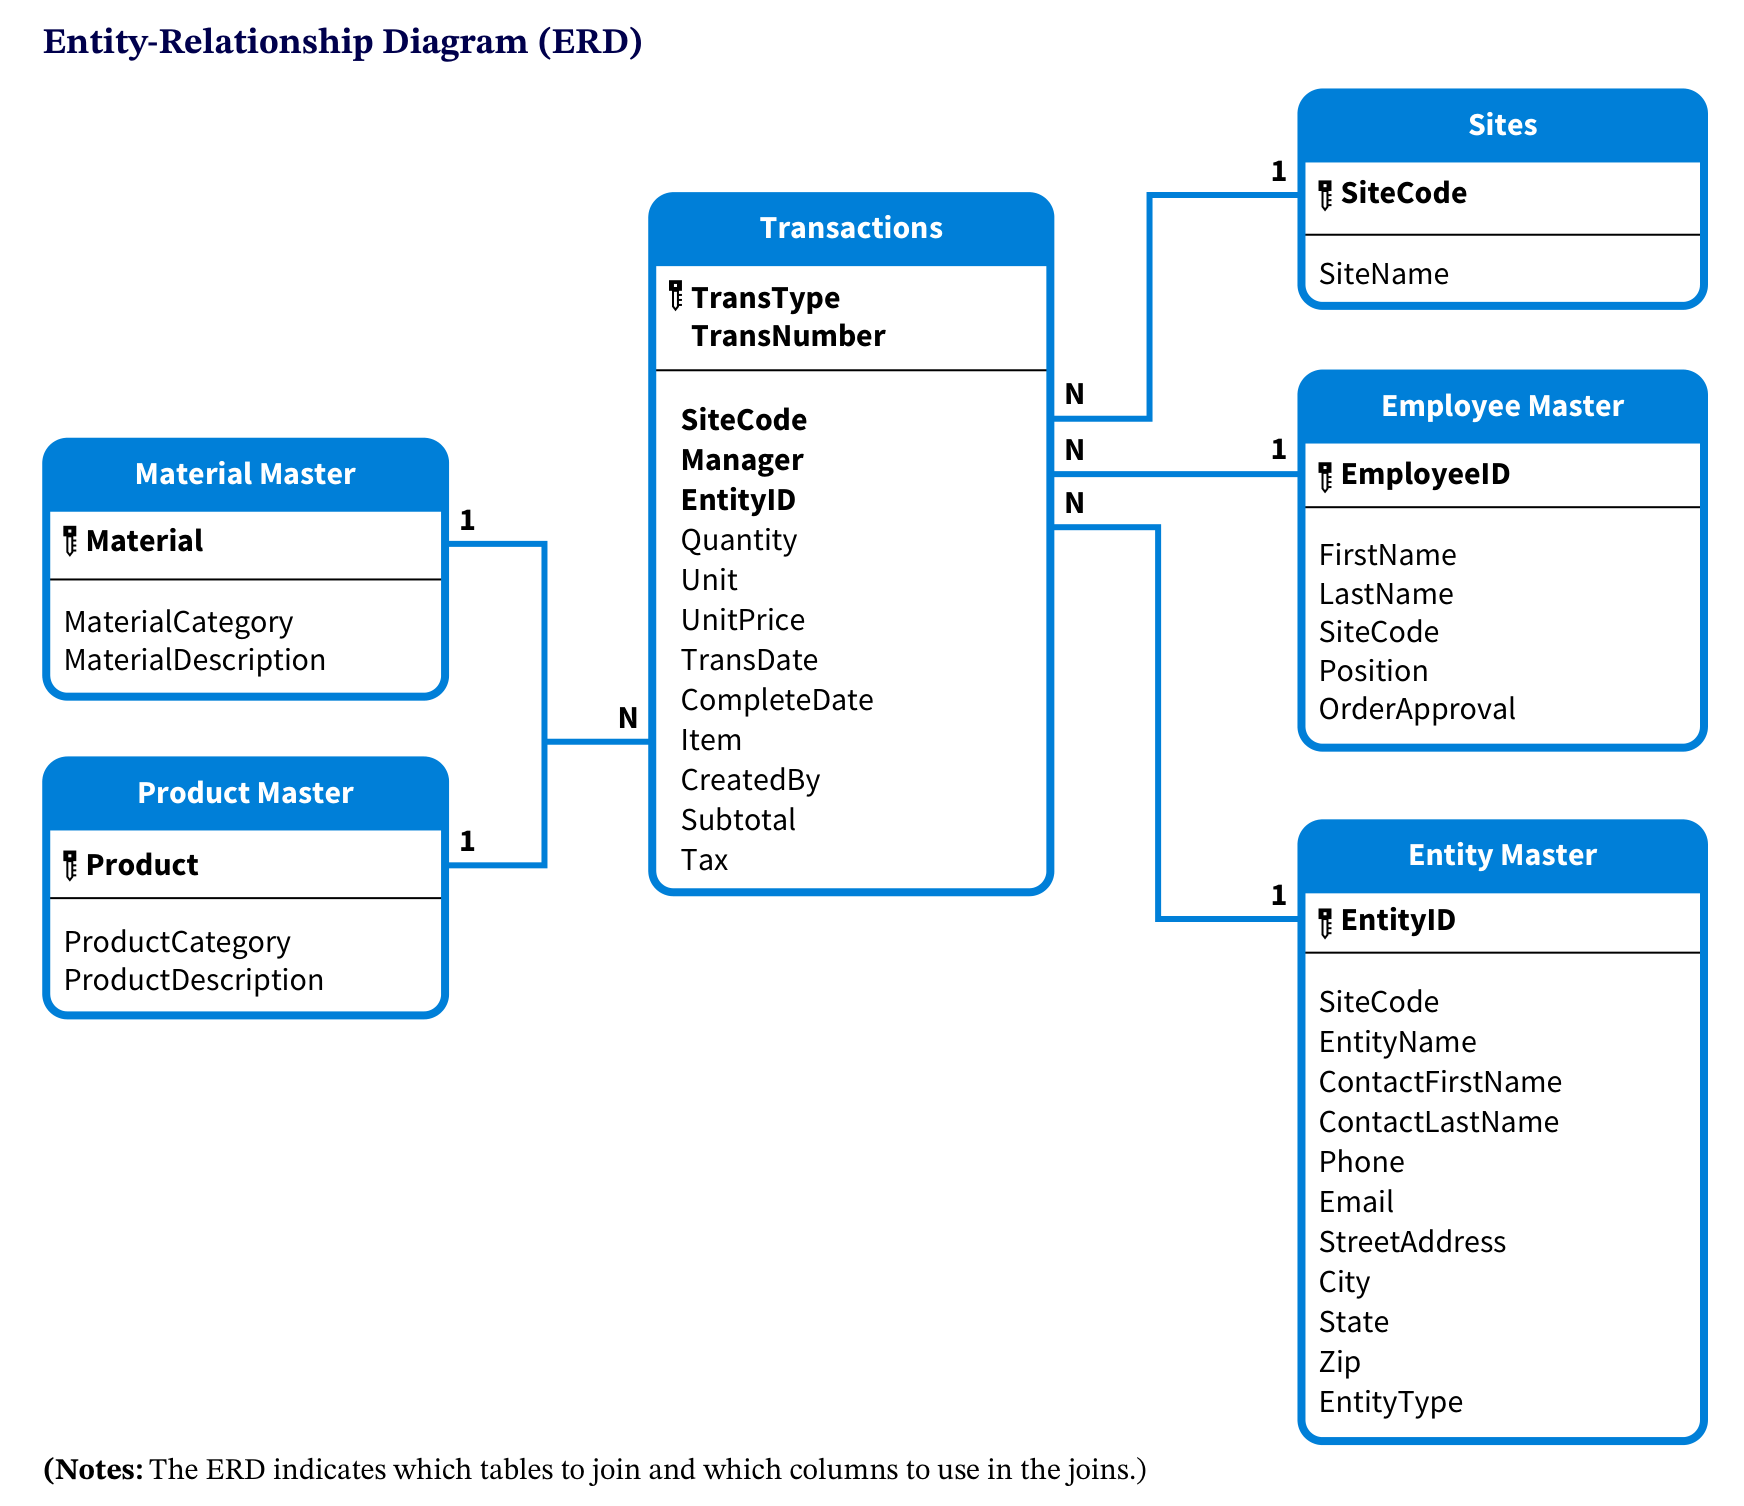
\includegraphics[width=0.95\textwidth,height=0.75\textheight,keepaspectratio]{../textbookForPractice/Figures/Ch_08/ERD 8.1A.png}
    \end{figure}
\end{frame}

\begin{frame}{ERD 8.1B}

    \begin{figure}[h]
        \centering
        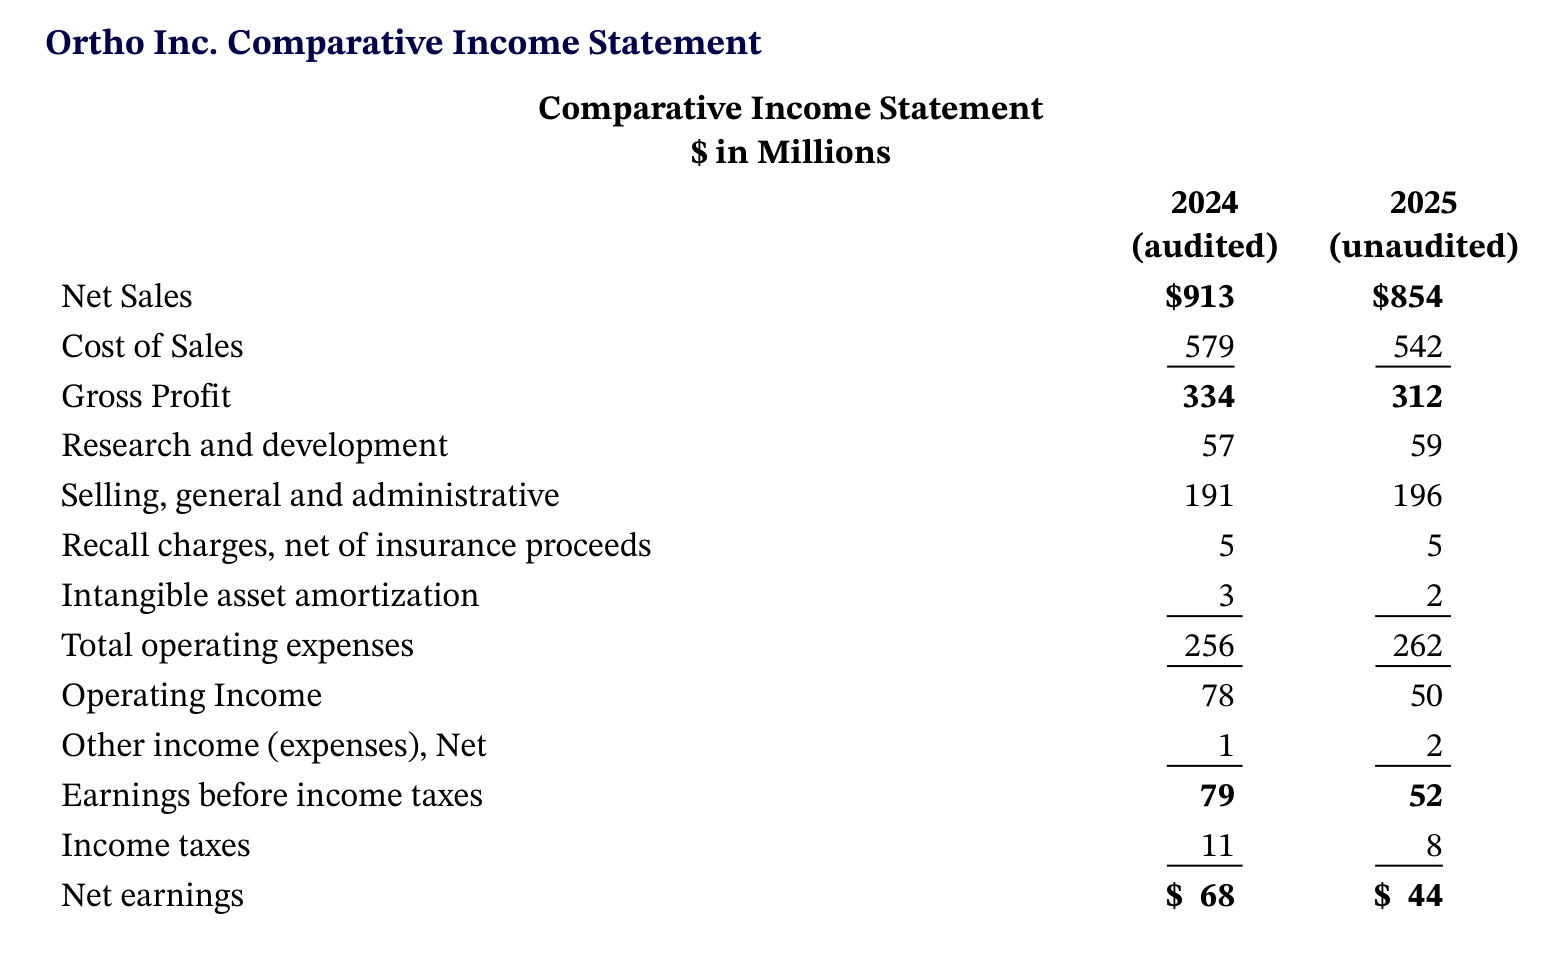
\includegraphics[width=0.95\textwidth,height=0.75\textheight,keepaspectratio]{../textbookForPractice/Figures/Ch_08/ERD 8.1B.png}
    \end{figure}
\end{frame}

\begin{frame}{Ortho Inc 8.1}

    \begin{figure}[h]
        \centering
        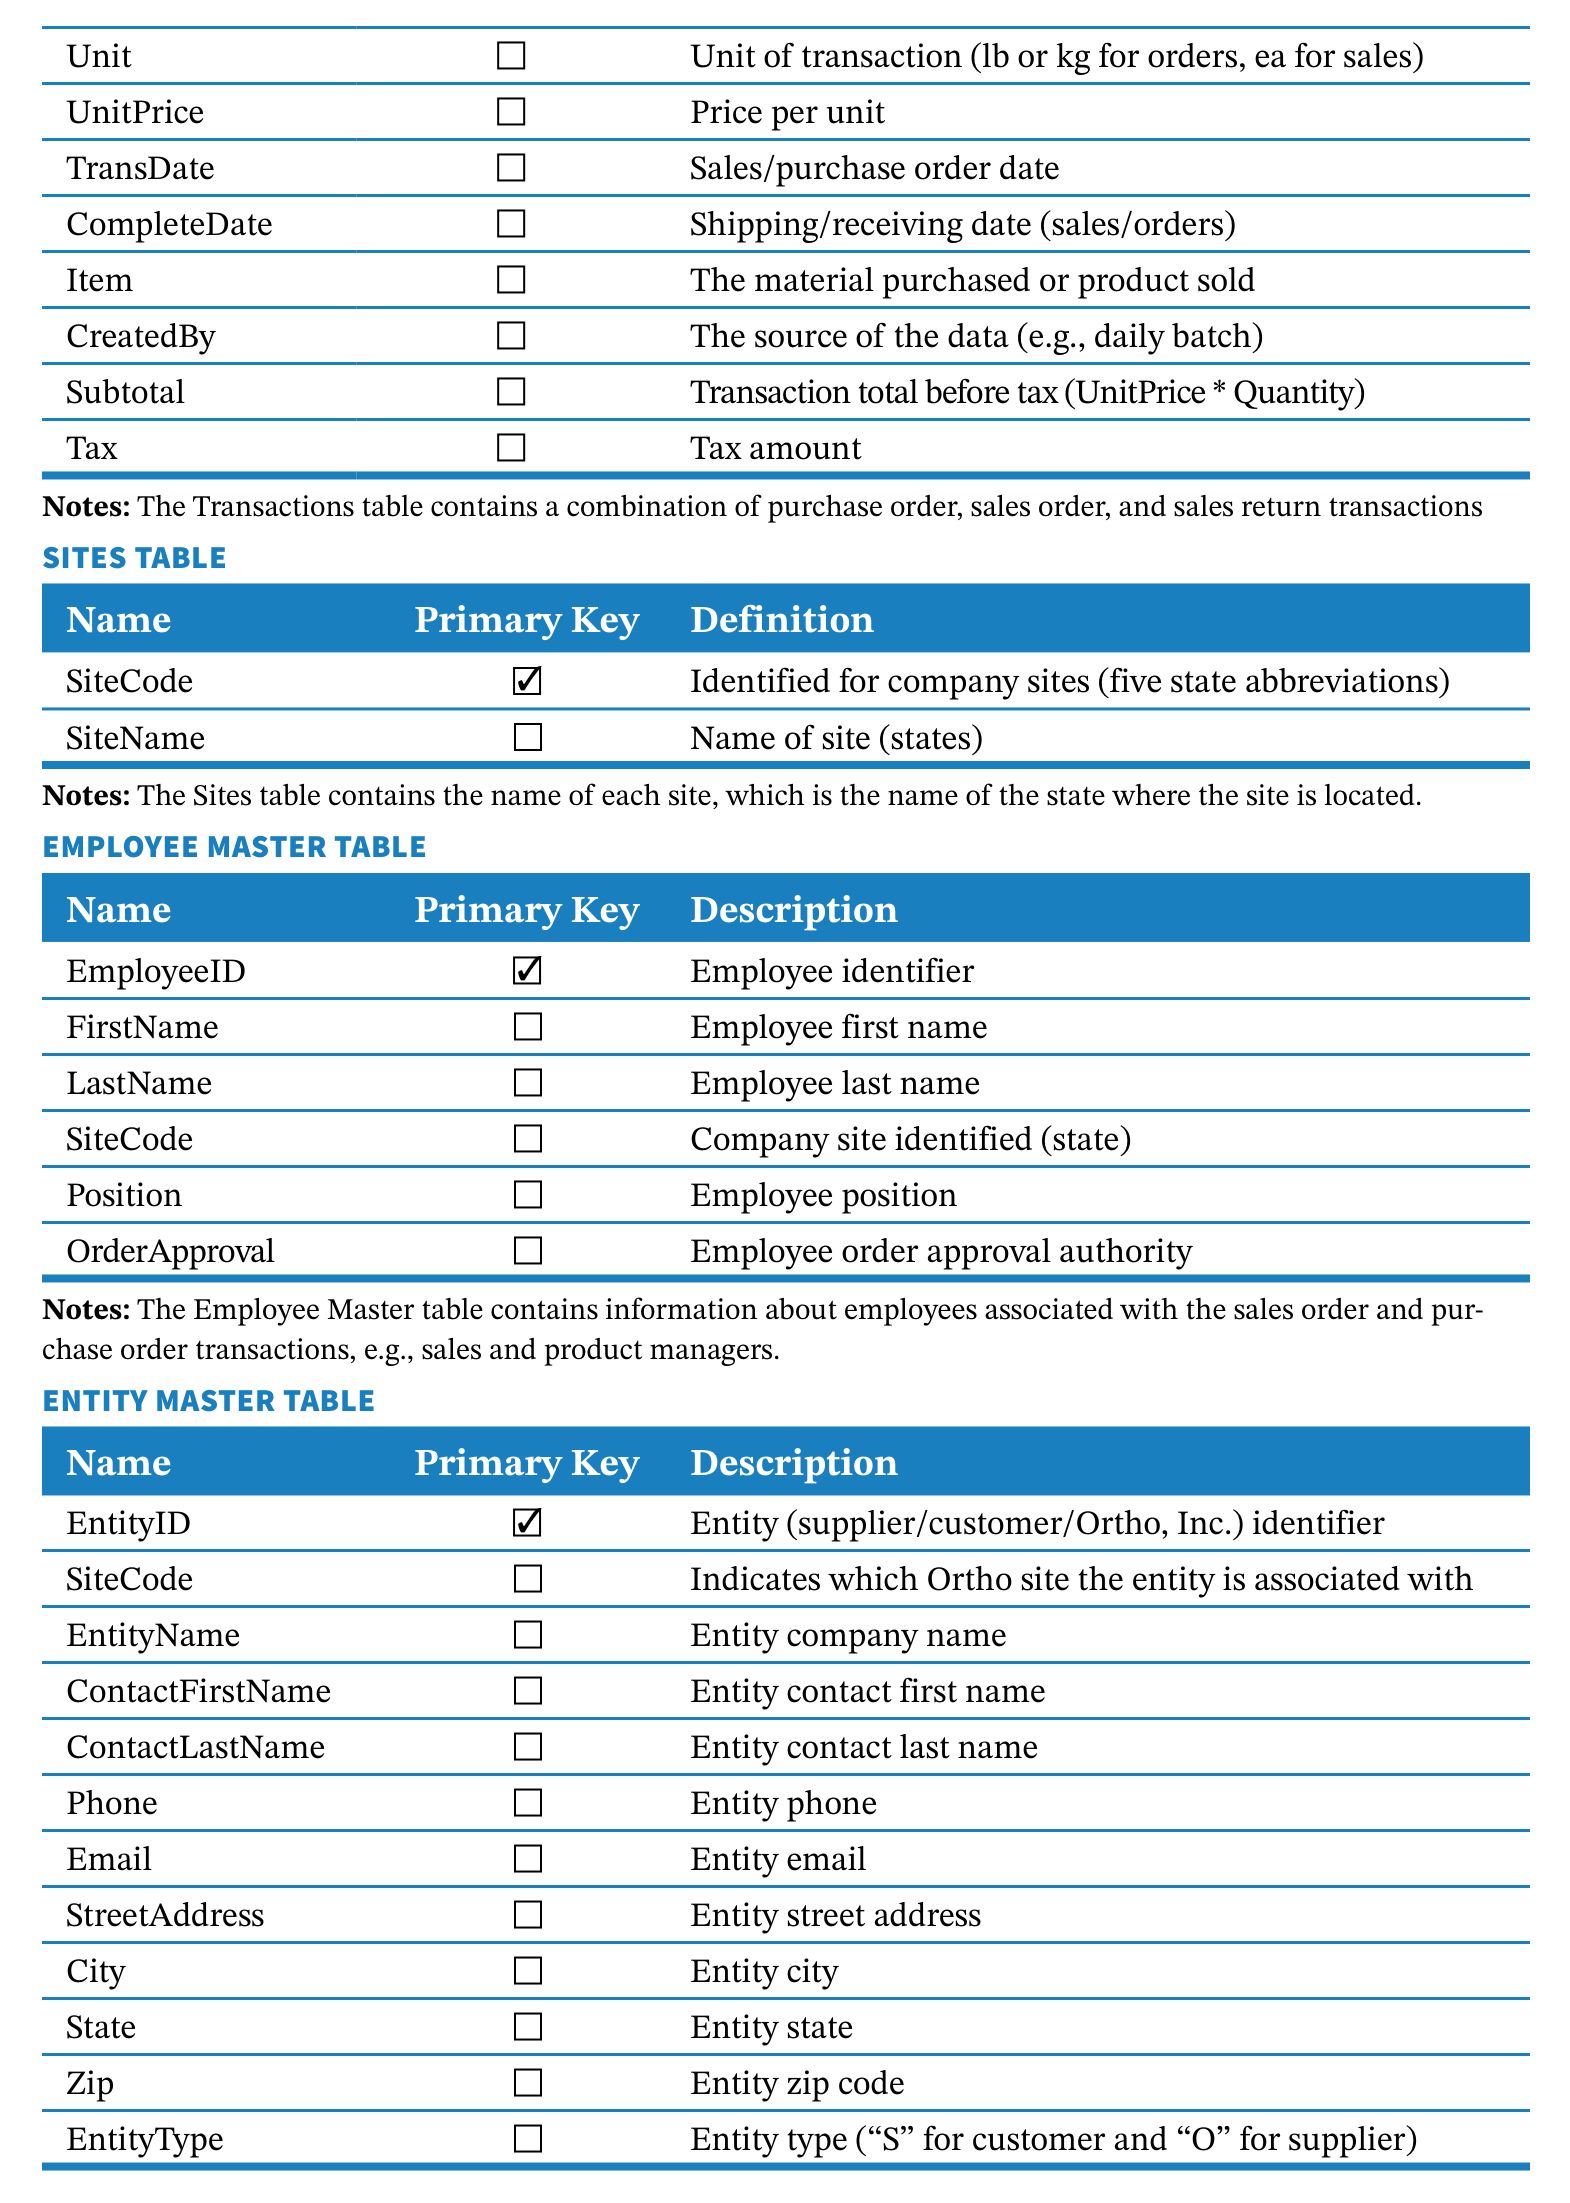
\includegraphics[width=0.95\textwidth,height=0.75\textheight,keepaspectratio]{../textbookForPractice/Figures/Ch_08/Ortho Inc 8.1.png}
    \end{figure}
\end{frame}

\begin{frame}{PR 8.1}

    \begin{figure}[h]
        \centering
        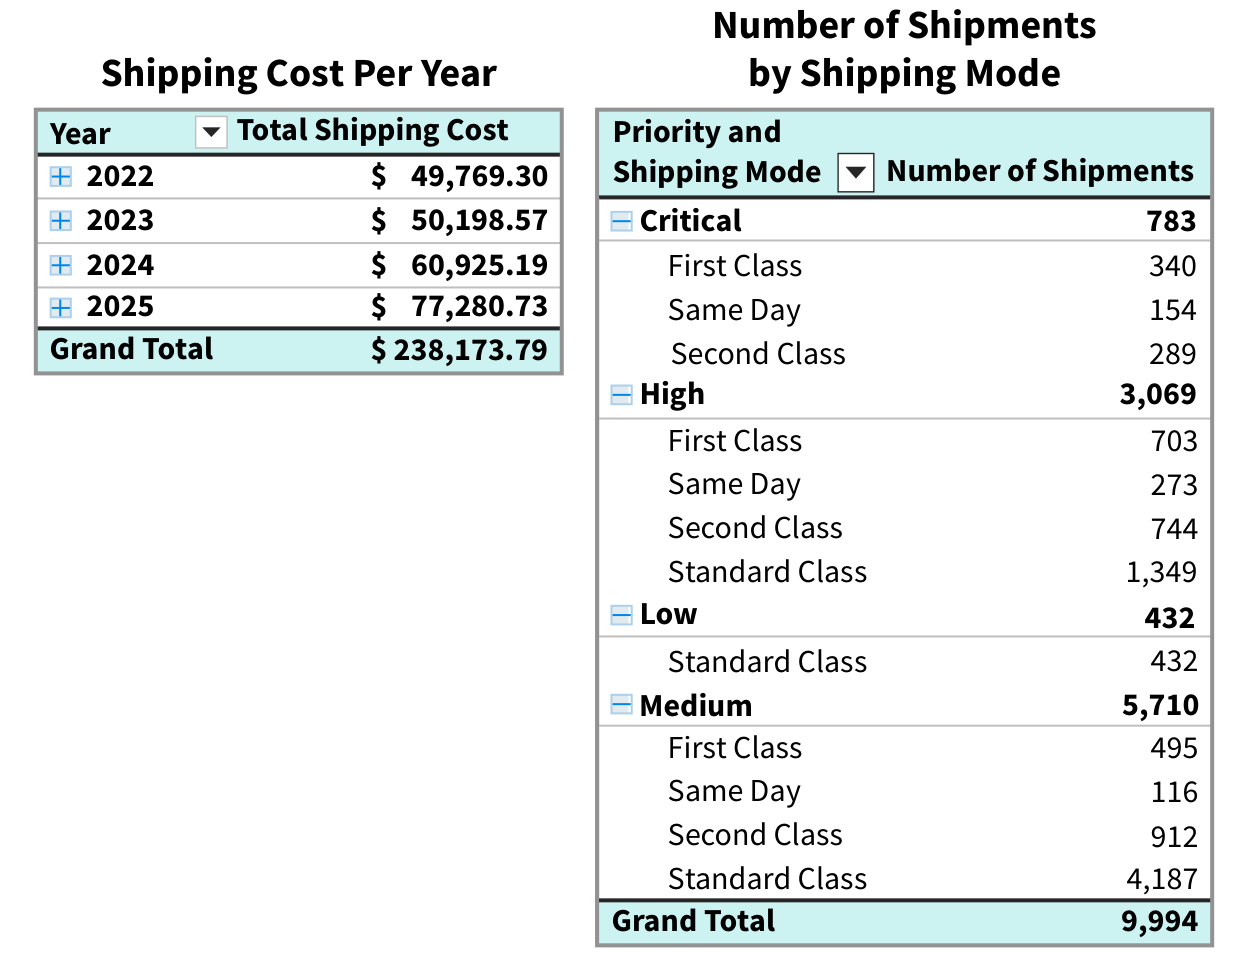
\includegraphics[width=0.95\textwidth,height=0.75\textheight,keepaspectratio]{../textbookForPractice/Figures/Ch_08/PR 8.1.png}
    \end{figure}
\end{frame}

\begin{frame}{Apply It 8.1A\_1}

    \begin{figure}[h]
        \centering
        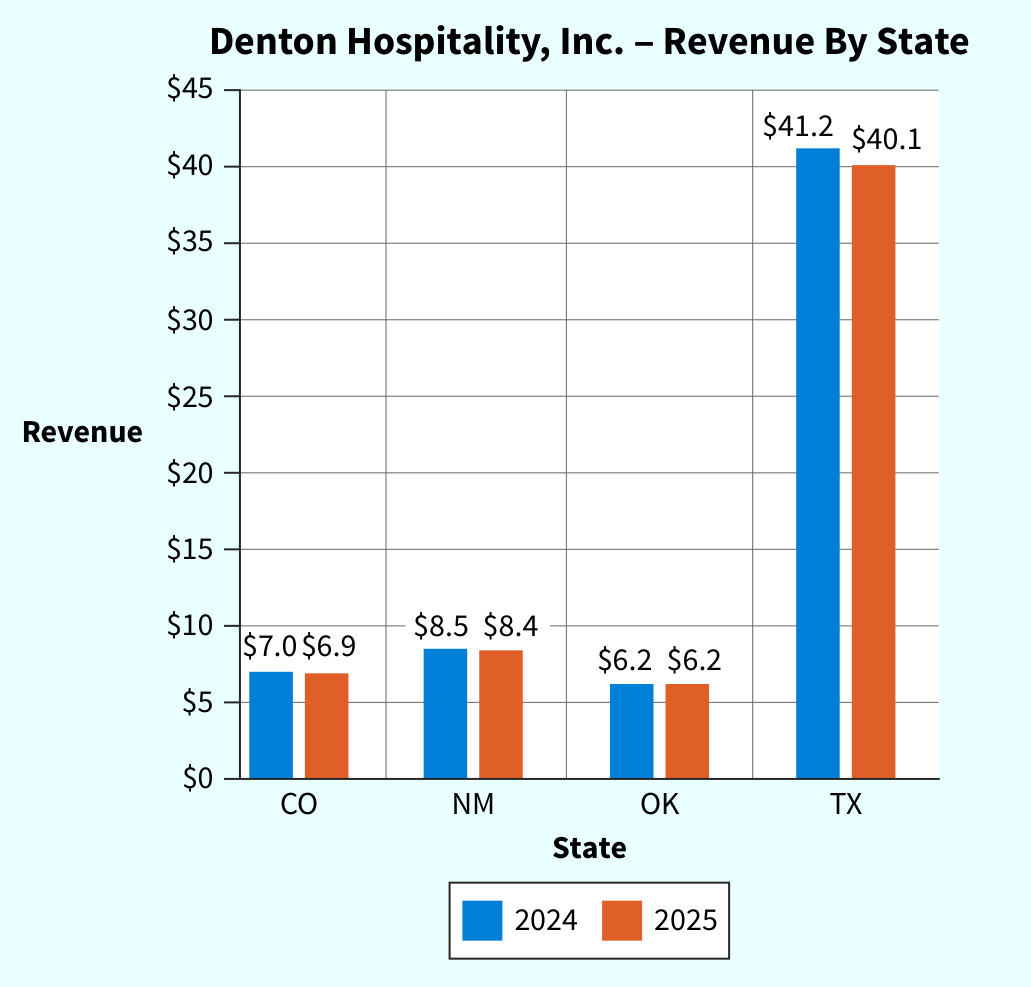
\includegraphics[width=0.95\textwidth,height=0.75\textheight,keepaspectratio]{../textbookForPractice/Figures/Ch_08/Apply It 8.1A_1.png}
    \end{figure}
\end{frame}

\begin{frame}{PR 8.2A}

    \begin{figure}[h]
        \centering
        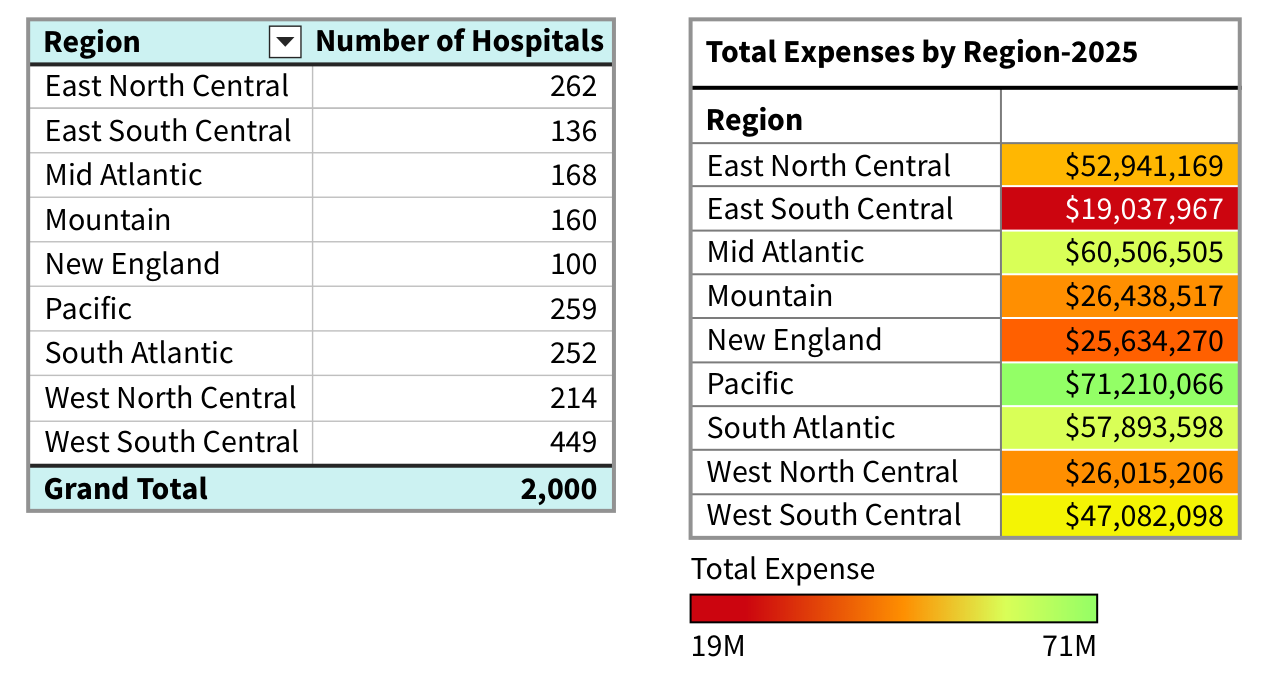
\includegraphics[width=0.95\textwidth,height=0.75\textheight,keepaspectratio]{../textbookForPractice/Figures/Ch_08/PR 8.2A.png}
    \end{figure}
\end{frame}

\begin{frame}{PR 8.2B}

    \begin{figure}[h]
        \centering
        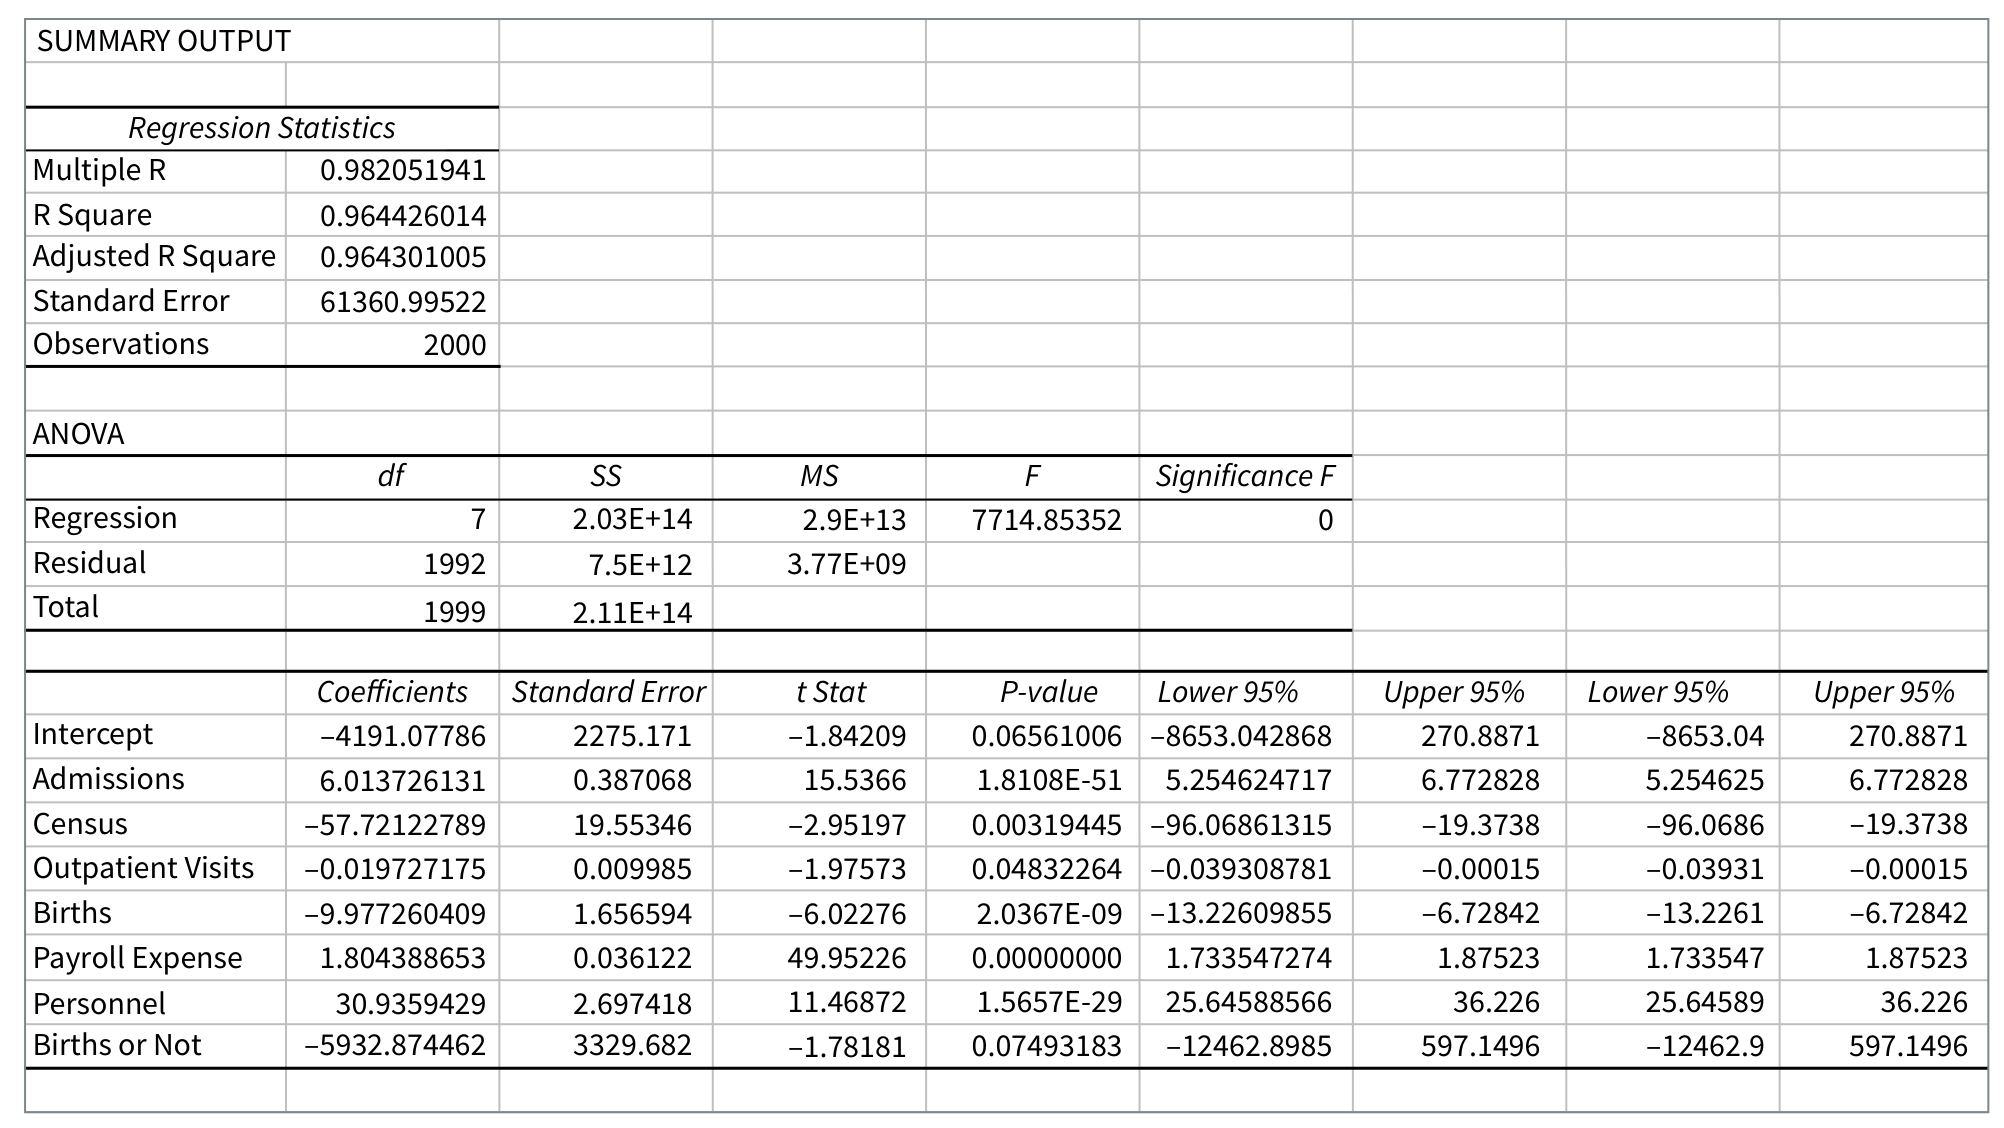
\includegraphics[width=0.95\textwidth,height=0.75\textheight,keepaspectratio]{../textbookForPractice/Figures/Ch_08/PR 8.2B.png}
    \end{figure}
\end{frame}

\begin{frame}{Apply It 8.3}

    \begin{figure}[h]
        \centering
        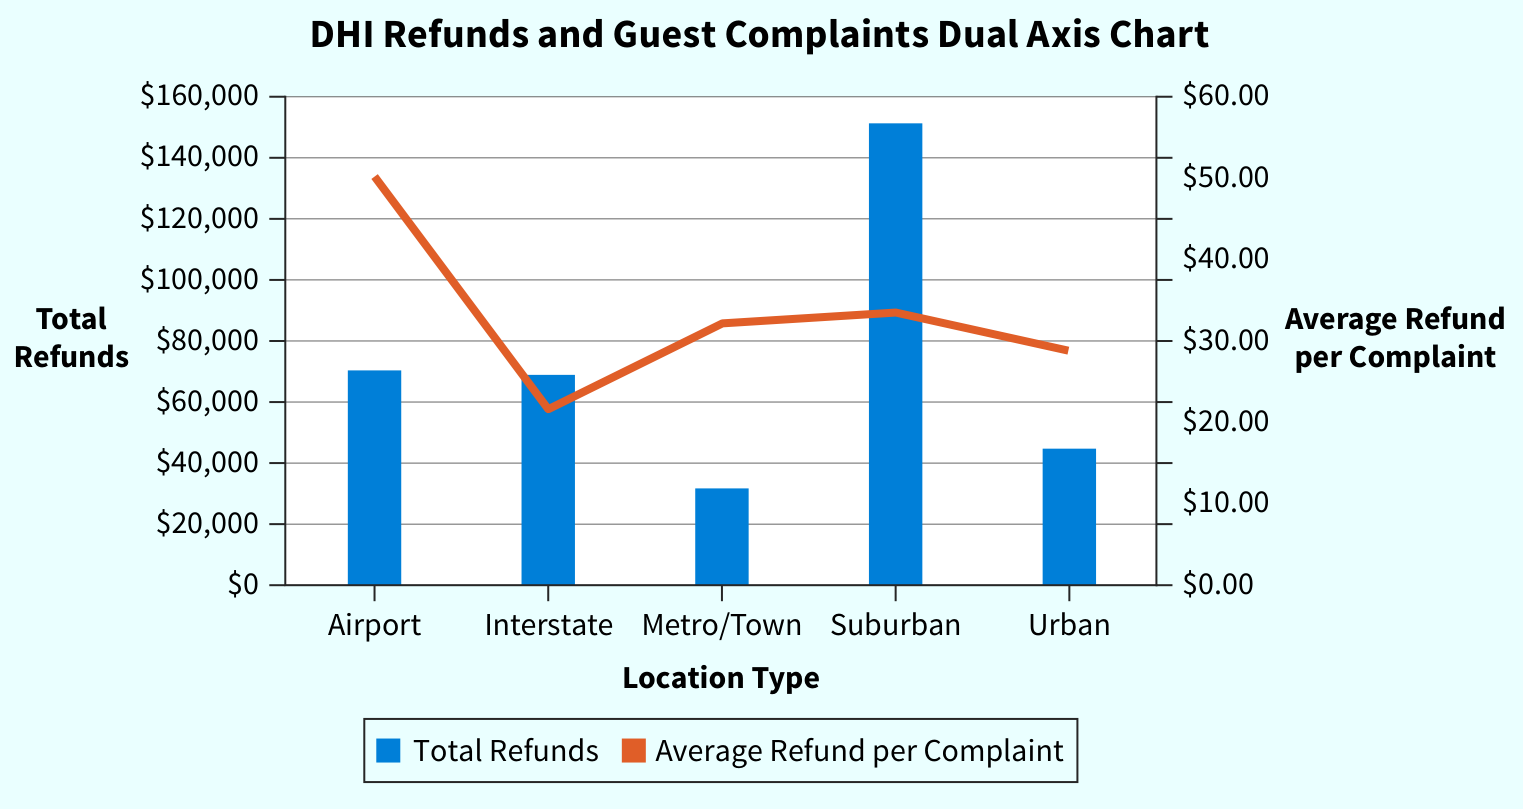
\includegraphics[width=0.95\textwidth,height=0.75\textheight,keepaspectratio]{../textbookForPractice/Figures/Ch_08/Apply It 8.3.png}
    \end{figure}
\end{frame}

\begin{frame}{Apply It 8.4}

    \begin{figure}[h]
        \centering
        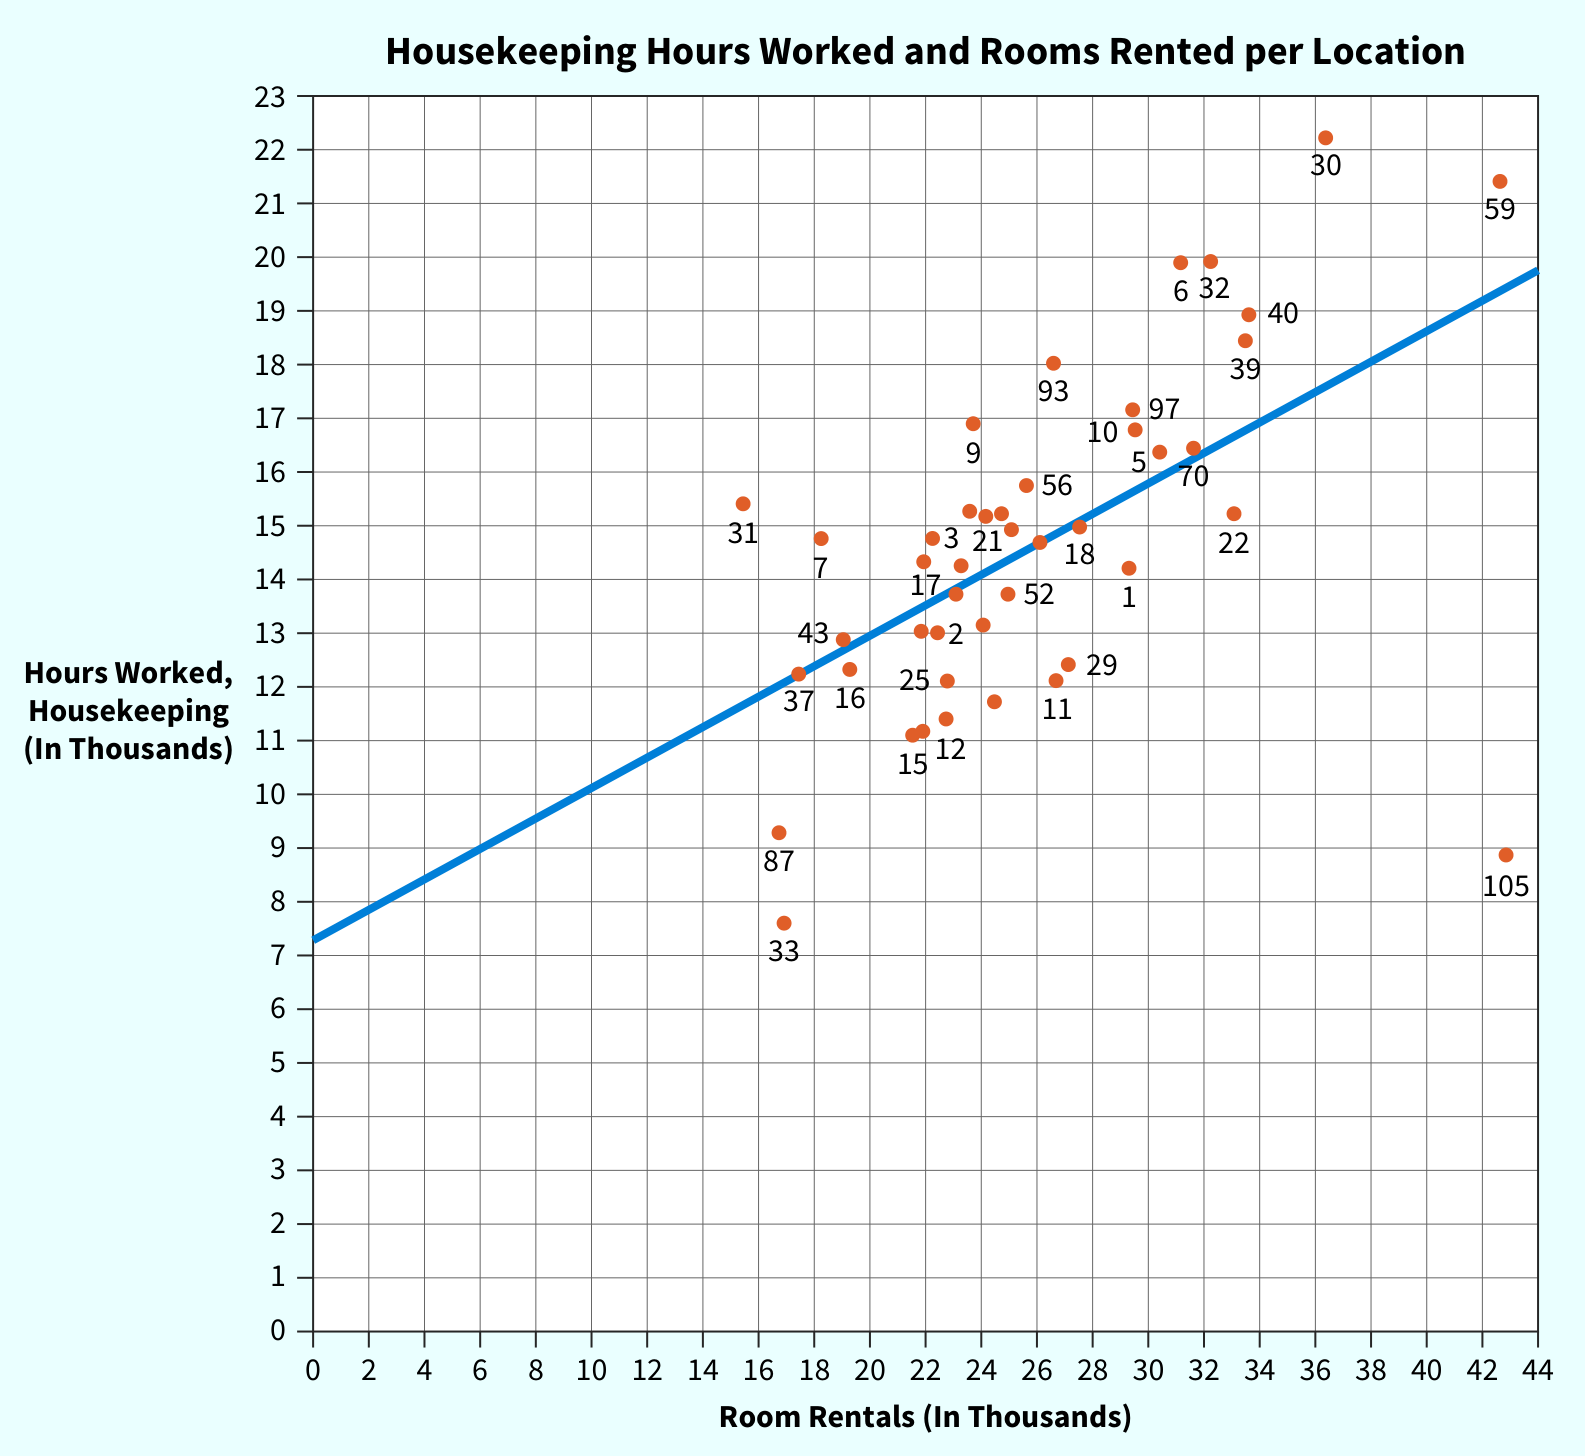
\includegraphics[width=0.95\textwidth,height=0.75\textheight,keepaspectratio]{../textbookForPractice/Figures/Ch_08/Apply It 8.4.png}
    \end{figure}
\end{frame}

\begin{frame}{Apply It 8.5}

    \begin{figure}[h]
        \centering
        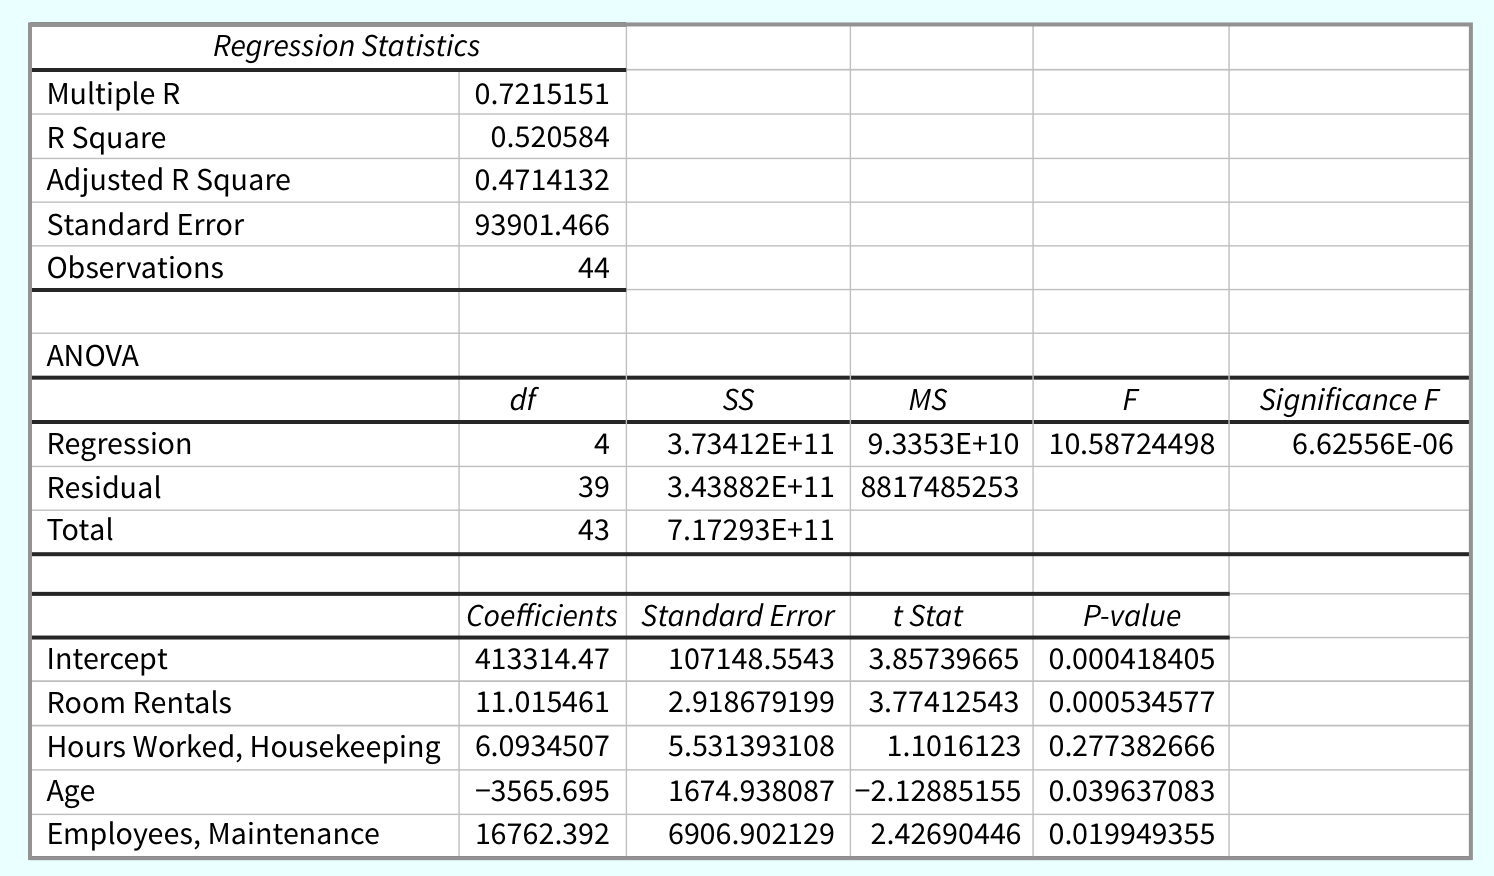
\includegraphics[width=0.95\textwidth,height=0.75\textheight,keepaspectratio]{../textbookForPractice/Figures/Ch_08/Apply It 8.5.png}
    \end{figure}
\end{frame}

\begin{frame}{Kết thúc}
    \begin{center}
        \Huge \textbf{Hỏi \& Đáp} \\
        \vspace{1cm}
        \Large Cảm ơn các bạn đã lắng nghe!
    \end{center}
\end{frame}

\end{document}
